% !TeX encoding = UTF-8
% !TeX program = xelatex
% !TeX spellcheck = en_US

\documentclass[degree=bachelor, fontset=windows]{thuthesis}
  % 学位 degree:
  %   doctor | master | bachelor | postdoc
  % 学位类型 degree-type:
  %   academic(默认)| professional
  % 语言 language
  %   chinese(默认)| english
  % 字体库 fontset
  %   windows | mac | fandol | ubuntu
  % 建议终版使用 Windows 平台的字体编译


% 论文基本配置,加载宏包等全局配置
% !TeX root = ./thuthesis-example.tex

% 论文基本信息配置

\thusetup{
  %******************************
  % 注意:
  %   1. 配置里面不要出现空行
  %   2. 不需要的配置信息可以删除
  %   3. 建议先阅读文档中所有关于选项的说明
  %******************************
  %
  % 输出格式
  %   选择打印版(print)或用于提交的电子版(electronic),前者会插入空白页以便直接双面打印
  %
  output = print,
  % 格式类型
  %   默认为论文(thesis),也可以设置为开题报告(proposal)
  % thesis-type = proposal,
  %
  % 标题
  %   可使用“\\”命令手动控制换行
  %
  title  = {基于定量中药组成数据和机器\\学习的中药靶点预测},
  title* = {Prediction of Traditional Chinese Medicine Targets Based on Quantitative Composition Data of Chinese Herbs and Machine Learning},
  %
  % 学科门类
  %   1. 学术型
  %      - 中文
  %        需注明所属的学科门类,例如:
  %        哲学、经济学、法学、教育学、文学、历史学、理学、工学、农学、医学、
  %        军事学、管理学、艺术学
  %      - 英文
  %        博士:Doctor of Philosophy
  %        硕士:
  %          哲学、文学、历史学、法学、教育学、艺术学门类,公共管理学科
  %          填写“Master of Arts“,其它填写“Master of Science”
  %   2. 专业型
  %      直接填写专业学位的名称,例如:
  %      教育博士、工程硕士等
  %      Doctor of Education, Master of Engineering
  %   3. 本科生不需要填写
  %
  % degree-category  = {工学硕士},
  % degree-category* = {Master of Science},
  %
  % 培养单位
  %   填写所属院系的全名
  %
  department = {探微书院},
  %
  % 学科
  %   1. 研究生学术型学位,获得一级学科授权的学科填写一级学科名称,其他填写二级学科名称
  %   2. 本科生填写专业名称,第二学位论文需标注“(第二学位)”
  %
  discipline  = {化学生物学(药学方向)},
  discipline* = {Chemical Biology for Pharmaceutical Sciences},
  %
  % 专业领域
  %   1. 设置专业领域的专业学位类别,填写相应专业领域名称
  %   2. 2019 级及之前工程硕士学位论文,在 `engineering-field` 填写相应工程领域名称
  %   3. 其他专业学位类别的学位论文无需此信息
  %
  % professional-field  = {计算机技术},
  % professional-field* = {Computer Technology},
  %
  % 姓名
  %
  author  = {洪宇睿},
  author* = {Yurui Hong},
  %
  % 学号
  % 仅当书写开题报告时需要(同时设置 `thesis-type = proposal')
  %
  % student-id = {2000310000},
  %
  % 指导教师
  %   中文姓名和职称之间以英文逗号“,”分开,下同
  %
  supervisor  = {李梢, 教授},
  supervisor* = {Professor Shao Li},
  %
  % 副指导教师
  %
  % associate-supervisor  = {陈文光, 教授},
  % associate-supervisor* = {Professor Chen Wenguang},
  %
  % 联合指导教师
  %
  % co-supervisor  = {某某某, 教授},
  % co-supervisor* = {Professor Mou Moumou},
  %
  % 日期
  %   使用 ISO 格式;默认为当前时间
  %
  % date = {2019-07-07},
  %
  % 是否在中文封面后的空白页生成书脊(默认 false)
  %
  include-spine = false,
  %
  % 密级和年限
  %   秘密, 机密, 绝密
  %
  % secret-level = {秘密},
  % secret-year  = {10},
  %
  % 博士后专有部分
  %
  % clc                = {分类号},
  % udc                = {UDC},
  % id                 = {编号},
  % discipline-level-1 = {计算机科学与技术},  % 流动站(一级学科)名称
  % discipline-level-2 = {系统结构},          % 专业(二级学科)名称
  % start-date         = {2011-07-01},        % 研究工作起始时间
}

% 载入所需的宏包

% 定理类环境宏包
\usepackage{amsthm}
% 也可以使用 ntheorem
% \usepackage[amsmath,thmmarks,hyperref]{ntheorem}

\thusetup{
  %
  % 数学字体
  % math-style = GB,  % GB | ISO | TeX
  math-font  = xits,  % stix | xits | libertinus
}

% 可以使用 nomencl 生成符号和缩略语说明
% \usepackage{nomencl}
% \makenomenclature

% 表格加脚注
\usepackage{threeparttable}

% 表格中支持跨行
\usepackage{multirow}

% 固定宽度的表格。
% \usepackage{tabularx}

% 跨页表格
\usepackage{longtable}

% 算法
\usepackage{algorithm}
\usepackage{algorithmic}

% 量和单位
\usepackage{siunitx}

% 参考文献使用 BibTeX + natbib 宏包
% 顺序编码制
% \usepackage[sort]{natbib}
% \bibliographystyle{thuthesis-numeric}

% 著者-出版年制
% \usepackage{natbib}
% \bibliographystyle{thuthesis-author-year}

% 生命科学学院要求使用 Cell 参考文献格式(2023 年以前使用 author-date 格式)
% \usepackage{natbib}
% \bibliographystyle{cell}

% 本科生参考文献的著录格式
\usepackage[sort]{natbib}
\bibliographystyle{thuthesis-bachelor}

% 参考文献使用 BibLaTeX 宏包
% \usepackage[style=thuthesis-numeric]{biblatex}
% \usepackage[style=thuthesis-author-year]{biblatex}
% \usepackage[style=gb7714-2015]{biblatex}
% \usepackage[style=apa]{biblatex}
% \usepackage[style=mla-new]{biblatex}
% 声明 BibLaTeX 的数据库
% \addbibresource{ref/refs.bib}

% 定义所有的图片文件在 figures 子目录下
\graphicspath{{figures/}}

% 数学命令
\makeatletter
\newcommand\dif{%  % 微分符号
  \mathop{}\!%
  \ifthu@math@style@TeX
    d%
  \else
    \mathrm{d}%
  \fi
}
\makeatother

% hyperref 宏包在最后调用
\usepackage{hyperref}

\usepackage{listings}

\begin{document}

% 封面
\maketitle

% 学位论文指导小组、公开评阅人和答辩委员会名单
% 本科生不需要
% \input{data/committee}

% 使用授权的说明
% 本科生开题报告不需要
% \copyrightpage
% 将签字扫描后授权文件 scan-copyright.pdf 替换原始页面
% \copyrightpage[file=scan-copyright.pdf]

\frontmatter
% !TeX root = ../thuthesis-example.tex

% 中英文摘要和关键字

\begin{abstract}
  本研究旨在应用机器学习方法,基于中药化合物定量组成数据,对其作用靶点进行预测,并进行实验验证。中药天然产物构成了一个广阔而有用的化学空间,对药物活性分子的研究提供了丰富的资源。然而,中药组成数据的定量面临内在难度、现状、方法等诸多挑战,而中药靶点预测任务除了受定量效果影响外,还存在建模表征预测能力不足的问题。本研究通过收集和标准化《中国药典》收录的中药化合物的定量数据,应用统计学和机器学习方法,使用图模型进行建模,尝试对药方合理性进行评估,以此对处方发现和优化在一定程度上进行辅助和检验。

  % 关键词用“英文逗号”分隔,输出时会自动处理为正确的分隔符
  \thusetup{
    keywords = {中医药天然产物, 药物发现, 中药组成定量, 图模型, 中药靶点预测},
  }
\end{abstract}

\begin{abstract*}
  This study aims to apply machine learning methods to predict the action targets of traditional Chinese medicine (TCM) based on the quantitative composition data of TCM compounds, followed by experimental validation. The natural products of TCM constitute a broad and useful chemical space, offering rich resources for the study of pharmacologically active molecules. However, the quantification of TCM composition faces multiple challenges, including inherent difficulties, current status, and methodologies. Furthermore, the task of predicting TCM targets is impacted by the effectiveness of quantification and the insufficiency of modeling representation and predictive ability. In this study, we collected and standardized quantitative data on TCM compounds listed in the \textit{Chinese Pharmacopoeia}, applied statistical and machine learning methods, and utilized graph models to evaluate the rationality of prescriptions. This approach assists and verifies prescription discovery and optimization to some extent.

  % Use comma as separator when inputting
  \thusetup{
    keywords* = {Traditional Chinese Medicine Natural Products, Drug Discovery, Quantification of TCM Composition, Graph Models, TCM Target Prediction},
  }
\end{abstract*}


% 目录
\tableofcontents

% 插图和附表清单
% 本科生的插图索引和表格索引需要移至正文之后、参考文献前
% \listoffiguresandtables  % 插图和附表清单(仅限研究生)

% 符号对照表
% !TeX root = ../thuthesis-example.tex

\begin{denotation}[3cm]
  \item[AdaBoost]{自适应提升算法(Adaptive Boosting)}
  \item[API]{应用程序接口(Application Programming Interface)}
  \item[AUC]{曲线下面积(Area Under Curve)}
  \item[BERT]{双向编码器表示变换器(Bidirectional Encoder Representations from Transformers)}
  \item[ccTCM]{成分与化合物中药数据库(Component and Compound platform for Traditional Chinese Medicine)}
  \item[CNN]{卷积神经网络(Convolutional Neural Network)}
  \item[CRISPR/Cas9]{CRISPR相关蛋白9(CRISPR-associated protein 9)}
  \item[CS]{化学相似性(Chemical Similarity)}
  \item[D值]{Kolmogorov-Smirnov检验统计量}
  \item[dCas9]{失活型Cas9蛋白(dead Cas9 protein)}
  \item[drugCIPHER-MS]{基于蛋白质网络的靶点预测回归模型定义的药物相似性}
  \item[GCN]{图卷积网络(Graph Convolutional Network)}
  \item[GNN]{图神经网络(Graph Neural Network)}
  \item[GPT]{生成式预训练模型(Generative Pre-trained Transformer)}
  \item[HTML]{超文本标记语言(HyperText Markup Language)}
  \item[LSTM]{长短时记忆网络(Long Short-Term Memory)}
  \item[NCBI Gene ID]{美国国家生物技术信息中心基因标识符(National Center for Biotechnology Information Gene Identifier)}
  \item[p值]{统计显著性水平}
  \item[PPI]{蛋白质-蛋白质相互作用(Protein-Protein Interaction)}
  \item[RNAi]{RNA干扰(RNA interference)}
  \item[RNN]{循环神经网络(Recurrent Neural Network)}
  \item[STRING]{互作基因/蛋白检索工具(数据库名称)}
  \item[TCM]{中医药(Traditional Chinese Medicine)}
  \item[Transformer]{变换器(一种深度学习模型)}
  \item[TS]{治疗相似性(Therapeutic Similarity)}
  \item[UniProt ID]{通用蛋白质标识符(Universal Protein Resource Identifier)}
\end{denotation}

% 也可以使用 nomencl 宏包,需要在导言区
% \usepackage{nomencl}
% \makenomenclature

% 在这里输出符号说明
% \printnomenclature[3cm]

% 在正文中的任意为都可以标题
% \nomenclature{PI}{聚酰亚胺}
% \nomenclature{MPI}{聚酰亚胺模型化合物,N-苯基邻苯酰亚胺}
% \nomenclature{PBI}{聚苯并咪唑}
% \nomenclature{MPBI}{聚苯并咪唑模型化合物,N-苯基苯并咪唑}
% \nomenclature{PY}{聚吡咙}
% \nomenclature{PMDA-BDA}{均苯四酸二酐与联苯四胺合成的聚吡咙薄膜}
% \nomenclature{MPY}{聚吡咙模型化合物}
% \nomenclature{As-PPT}{聚苯基不对称三嗪}
% \nomenclature{MAsPPT}{聚苯基不对称三嗪单模型化合物,3,5,6-三苯基-1,2,4-三嗪}
% \nomenclature{DMAsPPT}{聚苯基不对称三嗪双模型化合物(水解实验模型化合物)}
% \nomenclature{S-PPT}{聚苯基对称三嗪}
% \nomenclature{MSPPT}{聚苯基对称三嗪模型化合物,2,4,6-三苯基-1,3,5-三嗪}
% \nomenclature{PPQ}{聚苯基喹噁啉}
% \nomenclature{MPPQ}{聚苯基喹噁啉模型化合物,3,4-二苯基苯并二嗪}
% \nomenclature{HMPI}{聚酰亚胺模型化合物的质子化产物}
% \nomenclature{HMPY}{聚吡咙模型化合物的质子化产物}
% \nomenclature{HMPBI}{聚苯并咪唑模型化合物的质子化产物}
% \nomenclature{HMAsPPT}{聚苯基不对称三嗪模型化合物的质子化产物}
% \nomenclature{HMSPPT}{聚苯基对称三嗪模型化合物的质子化产物}
% \nomenclature{HMPPQ}{聚苯基喹噁啉模型化合物的质子化产物}
% \nomenclature{PDT}{热分解温度}
% \nomenclature{HPLC}{高效液相色谱(High Performance Liquid Chromatography)}
% \nomenclature{HPCE}{高效毛细管电泳色谱(High Performance Capillary lectrophoresis)}
% \nomenclature{LC-MS}{液相色谱-质谱联用(Liquid chromatography-Mass Spectrum)}
% \nomenclature{TIC}{总离子浓度(Total Ion Content)}
% \nomenclature{\textit{ab initio}}{基于第一原理的量子化学计算方法,常称从头算法}
% \nomenclature{DFT}{密度泛函理论(Density Functional Theory)}
% \nomenclature{$E_a$}{化学反应的活化能(Activation Energy)}
% \nomenclature{ZPE}{零点振动能(Zero Vibration Energy)}
% \nomenclature{PES}{势能面(Potential Energy Surface)}
% \nomenclature{TS}{过渡态(Transition State)}
% \nomenclature{TST}{过渡态理论(Transition State Theory)}
% \nomenclature{$\increment G^\neq$}{活化自由能(Activation Free Energy)}
% \nomenclature{$\kappa$}{传输系数(Transmission Coefficient)}
% \nomenclature{IRC}{内禀反应坐标(Intrinsic Reaction Coordinates)}
% \nomenclature{$\nu_i$}{虚频(Imaginary Frequency)}
% \nomenclature{ONIOM}{分层算法(Our own N-layered Integrated molecular Orbital and molecular Mechanics)}
% \nomenclature{SCF}{自洽场(Self-Consistent Field)}
% \nomenclature{SCRF}{自洽反应场(Self-Consistent Reaction Field)}



% 正文部分
\mainmatter
% !TeX root = ../thuthesis-example.tex

\chapter{引言}

\section{研究背景}
\subsection{中医药天然产物是药物发现中有价值的化学空间}

在药物发现领域,化学空间指的是通过特征和规则定义的潜在的药理学活性分子的空间,通过计算分子的特征来比对相似性,从而推测分子针对特定生物过程的活性。然而,在广阔的所有可能分子的空间中寻找有药物活性的分子是一项极具挑战性的任务。即使仅考虑符合里宾斯基五规则的小分子药物,也至少有$10^{60}$种可能的有机分子\cite{Kirkpatrick_Ellis_2004},这对实际的药物筛选是不可接受的。在现有的药物发现流程中,往往使用虚拟筛选方法,包括基于结构的药物设计和基于配体的药物设计。其中,前者要求具体的目标蛋白结构,需要首先根据生物学研究范式确定目标靶点,后者通过计算分子之间的相似性进行预测,但是结构相似性和生物活性之间的关系并不强烈甚至并不明确。因此,在这些方法的基础上,我们可能需要更多的先验来指导药物发现的探索过程,利用我国传统中草药的丰富资源就是一条可行的途径。一方面,中草药来自种类繁多的植物,其天然产物构成一个广阔的化学空间,为药物发现提供了搜索范围;另一方面,许多中草药的药理活性已经在中医药几千年的临床实践中得到验证,这些前人总结出的经验显示了中草药天然产物相比随机分子显著更高的成药可能\cite{发挥我国传统医药及资源优势进行创新药物的基础研究}。因此,以中草药天然产物为基础,可以为药物发现提供更多的先验知识。

相比传统基于单个候选分子与靶点作用的药物发现方法,从中草药出发进行探索还具有整体性、系统性的特点。中医药的理论与实践并不总是进行单一有效成分的提取、纯化和使用,而是将多种药材结合使用,形成“方剂”,有意让多种有效成分协同发挥作用\cite{网络药理学与中医药现代研究的若干进展_2015}。从现代生物学的角度看,中药方剂在发挥药效时,其中的多种有效成分可能作用于不同的靶点,从而在生物体内形成复杂的网络效应,整体对特定信号通路、生物过程产生调控作用。因此,从中草药出发进行药物发现,可以更好地利用这种调控网络的整体性、系统性,从而更好地发现临床意义上的新药。

\subsection{中药组成数据的定量}

中草药组成成分的确定和定量是新药研发中的重要一环。有了充足的定量数据,我们才得以比较药材成分,进行高通量筛选,应用统计学和机器学习方法寻找相关性,从而确定候选药材和分子。作为多组分天然产物,中草药的成分分析方法主要包括色谱法、质谱法、核磁共振法等\cite{中药有效部位及成分提取工艺和检测方法_2007}。在质量检测、产地溯源等实际应用的驱动下,已经形成了对特定中药材的检测仪器技术。然而,这一步骤并不容易。一方面,中草药的组成成分种类繁多,而同一药材在不同的生长环境下,其成分与含量也可能有所不同,这是问题本身的复杂性;另一方面,关于中草药的定量研究起步晚、规模小,而进行定量研究的成本高昂,效率较低,导致全国乃至世界范围内尚未形成统一的标准和完善的数据库。如下统计图\ref{fig:statistics}所示,现有的中医药数据库具有分散程度高、单个规模小,信息组织不够结构化的问题,这给中草药的定量研究带来了挑战\cite{Yang_Zhu_Yao_Chen_Chen_Gu_Jiang_Chen_Zhang_Wu_et_al._2023}。

\begin{figure}[H]
  \centering
  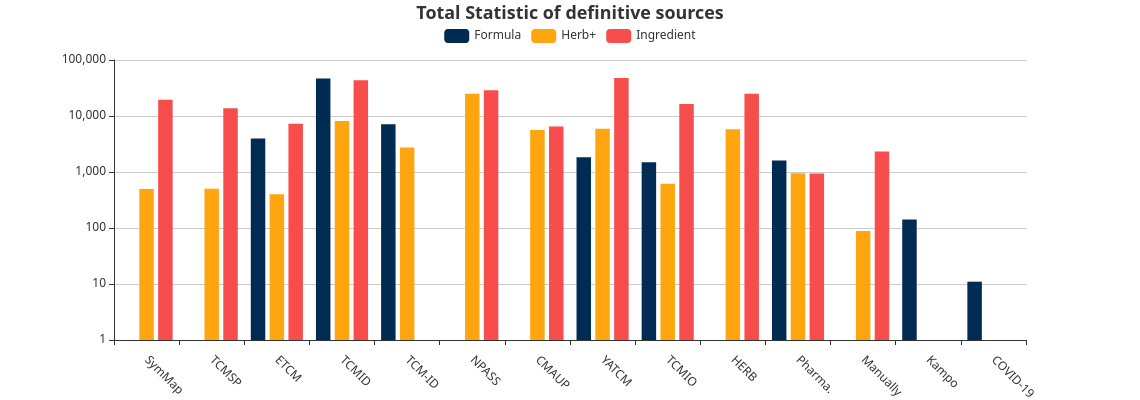
\includegraphics[width=\linewidth]{total_statistic_of_definitiv_sources.png}
  \caption{现有中药数据库的统计信息}
  \label{fig:statistics}
\end{figure}


为了应对这一挑战,除了期望中药数据库的发展完善外,我们可以通过主动收集数据和优化处理方法的方式进行解决。其中,主动收集数据包括对研究中重点关注的中草药进行直接定量分析,以及对已有的中草药成分定量数据进行整理、收集和标准化,从而形成一个可供后续研究使用的数据库。优化处理方法则包括选用合适的建模方法,如非参数统计方法、集成学习、迁移学习,或者利用先验补足数据的缺失,建立概率图模型来更好地利用有限的数据。此外,我们还可以使用临床实验数据和基于分子对接的计算方法来辅助中草药成分的定量研究。

\section{研究现状}

\subsection{中药靶点预测任务}

在中药组成数据的基础上,我们可以进行多种下游任务,如中药靶点预测、传统理论属性解释、中药剂量关系,乃至处方优化等。其中,本课题的重点是中药靶点预测。如果确定了针对某种具体疾病或表征有显著效果的天然产物分子,我们可以,通过直接查询已有的靶点数据库,进行化学相似性搜索、反向药效团搜索,或者应用反向分子对接的方法,利用三维建模测试分子与靶点的亲和力,从而预测分子的靶点。\cite{Huang_Zhang_Zhou_Lin_Chen_Lin_Mai_Huang_2018}然而,在更多的情形中,我们无法确定具体的药效分子,往往需要建立复杂的药物-靶点互作网络。面对中药相关数据量有限的问题,我们还可以进行药物-基因-疾病关联分析,建立概率图模型,将药物作用靶点建模成隐变量,通过这种一体化分析方法提高预测能力。目前,中药网络药理学的一大重要参考是本草组鉴(HERB)数据库,基于文本挖掘,辅以人工标定,结合数据库掘和统计推断,共将12,933个靶点28,212种疾病和7,263种中草药、49,258种成分联系起来,并提供了它们之间的六种配对关系。其中部分提供高通量实验证据、差异分析及富集分析结果\cite{Fang_Dong_Liu_Guo_Zhao_Zhang_Bu_Liu_Huo_Cao_et_al._2021}。虽然该数据库并不主要聚焦于我们关心的化合物定量信息,但其提供的众多关联信息,乃至丰富高通量实验和文献参考,也可作为我们建模时的参考。

\begin{figure}[H]
  \centering
  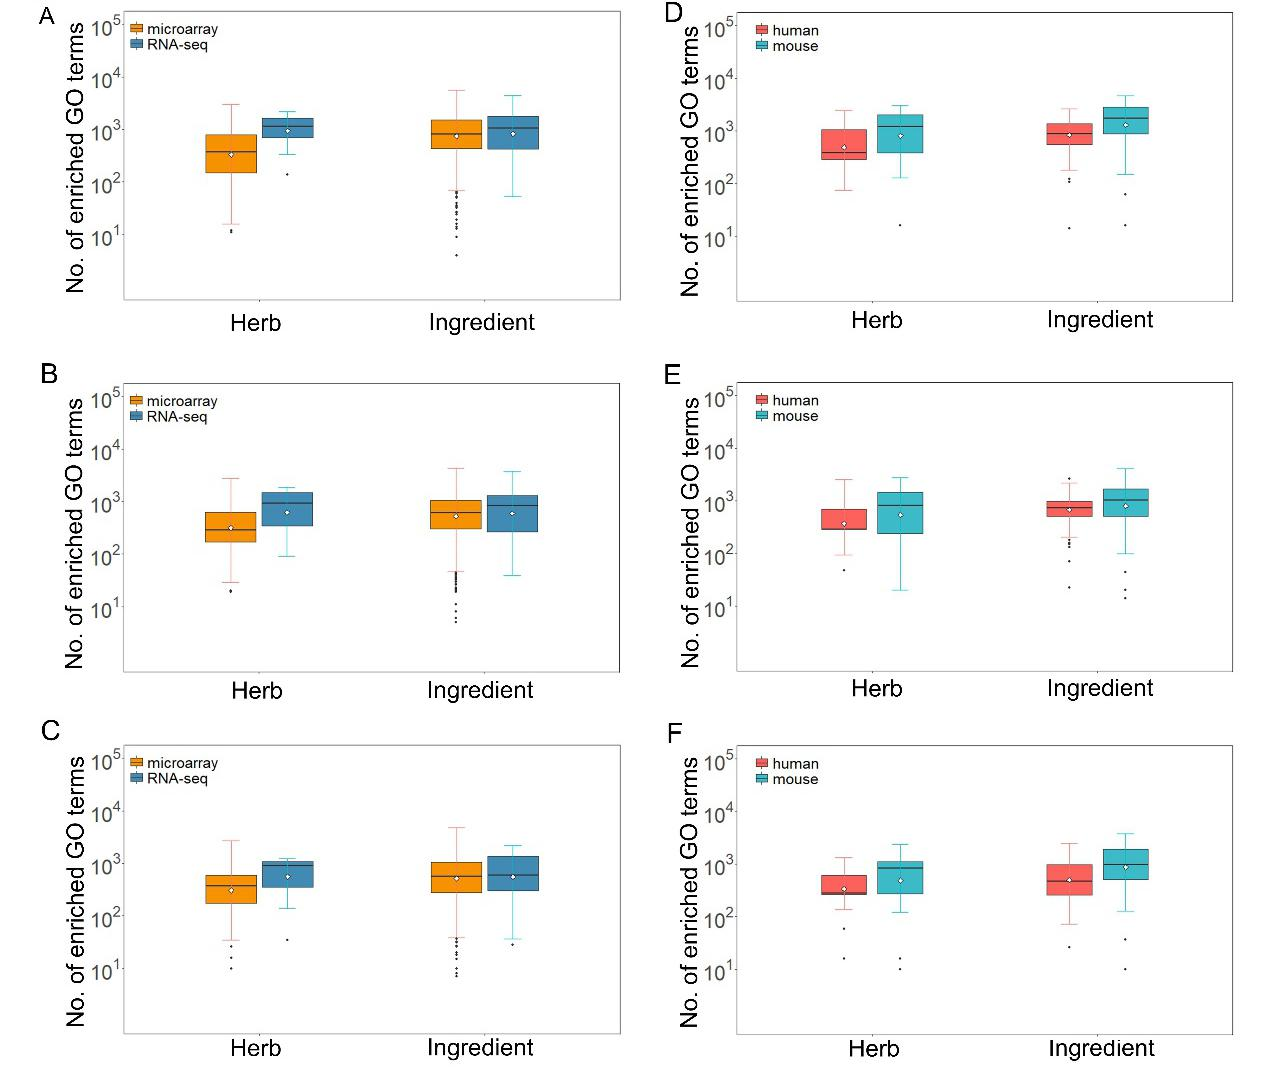
\includegraphics[width=\linewidth]{figures/HERB.png}
  \caption{HERB数据库提供的六种配对关系\cite{Fang_Dong_Liu_Guo_Zhao_Zhang_Bu_Liu_Huo_Cao_et_al._2021}}
  其中ABC/DEF分别基于微观/宏观实践结果,而AD/BE/CF分别展示差异/上调/下调基因
  \label{fig:HERB}
\end{figure}

在HERB之后,类似的数据库主要还有 ITCM 和 BATMAN-TCM,它们往往都从HERB中参考部分信息,或者将高通量结果与HERB进行对比印证。其中,ITCM进行了更大规模的实验,进行了基于转录组的多尺度分析以阐释机理,在验证HERB数据有效性的同时开发应用了6种前沿特征搜索方法,并将它们整合到名为 TCM-Query 的筛选策略中,以识别特殊疾病的潜在活性成分,同时通过文献挖掘进行了一额外补充\cite{Tian_Zhang_Yuan_Wang_Lv_Wang_Fang_Fu_Yang_Zu_et_al._2023};而BATMAN-TCM在手动补充中药成分-蛋白相互作用的基础上整合了探索中药成分的靶点从而探究药理、描述与蛋白的关联而辅助药物发现的功能\cite{Kong_Liu_Zhang_Cheng_Mei_Li_Liu_Diao_Ma_Jiang_et_al._2024}。这些研究的发展迭代速度很快,使得中药靶点预测的数据库工具数据日趋丰富,功能日趋完善。

\subsection{现有的靶标预测算法}

\subsubsection{基于分子指纹的结构相似性算法}

分子指纹是一种分子抽象表征的方法,通过一定的规则将分子由二维结构图压缩为一维比特向量。在恰当的映射方式下,分子指纹的公共片段可以表征原分子的局部结构相似性,从而将二维分子的比较转化为可在计算机中高效处理的一维向量比较。使用基于分子指纹的结构相似性算法进行靶标预测,就是在已有数据库的靶点配体分子中寻找与待预测分子结构相似的分子进行预测。根据分子指纹的生成方式,可以定义一系列的算法并建立相应数据库,如基于拓扑结构的Daylight分子指纹对应SEA数据库\cite{Keiser_Roth_Armbruster_Ernsberger_Irwin_Shoichet_2007},基于圆形子结构的ECFP分子指纹对应SuperPred数据库\cite{Nickel_Gohlke_Erehman_Banerjee_Rong_Goede_Dunkel_Preissner_2014}。这些算法在小分子预测任务上不断进行迭代开发,目前已经取得了较好的效果。

\subsubsection{多重相似性算法}

然而,上述基于化学结构的方法中的假设并不普遍正确,结构相似的药物可能结合无明显结构、序列相似性的靶点,而结构细节的微小差异就有可能造成对同一靶点截然不同的结合能力,这在分子对接中是可以验证的结论。因此,除了结构信息外,我们还可以引入基因表达上下游的其他信息,通过整合后的信息进行更加准确的判断。其中的一个典型代表是drugCIPHER-MS算法。在药理学空间内,这种方法在化学相似性(CS)之外从下游表型定义了一个治疗相似性(TS);除此以外,还引入了靶标蛋白质相关性的蛋白质-蛋白质相互作用(PPI)网络特征,从而建立了一个高维回归模型,充分整合各个层面的已知信息,从而提高了预测的准确性\cite{Zhao_Li_2010}。

\begin{figure}[H]
  \centering
  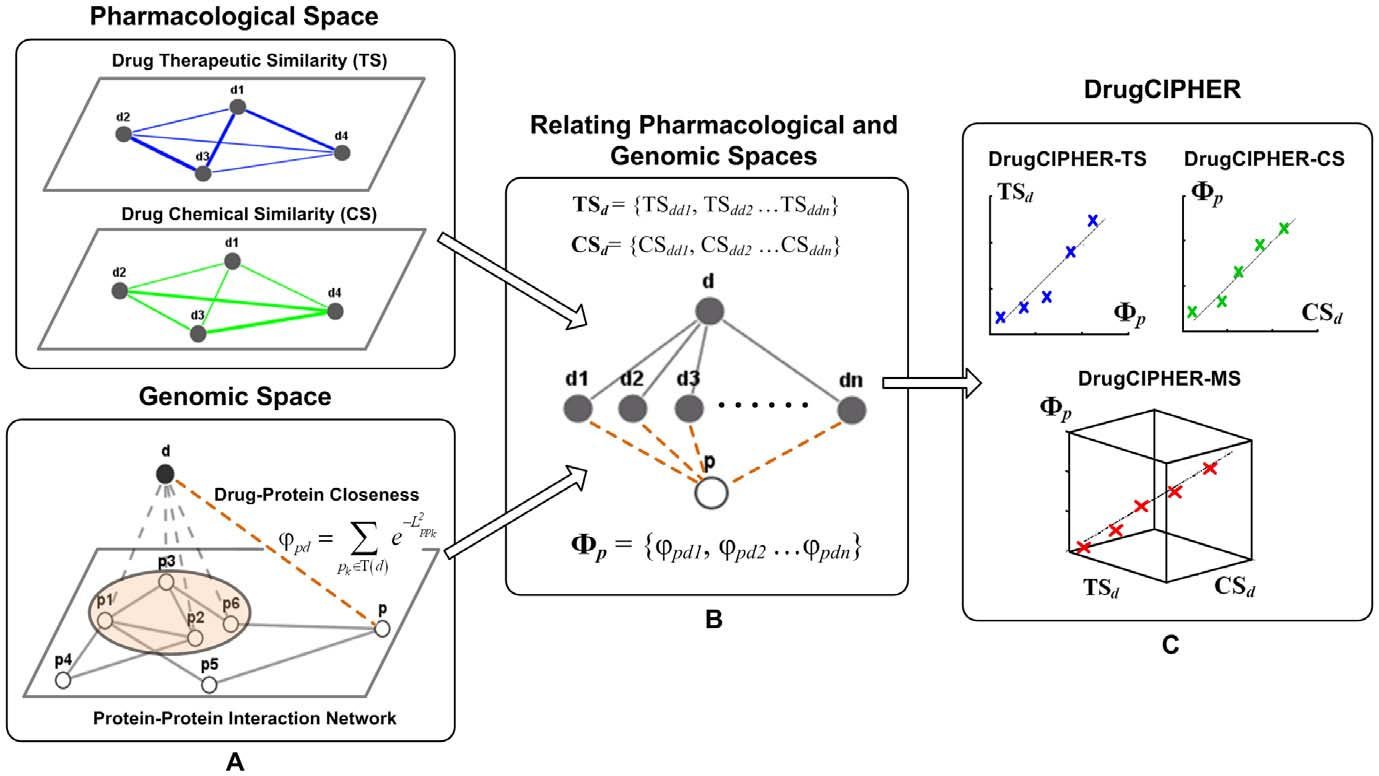
\includegraphics[width=\linewidth]{figures/drugCIPHER-MS.png}
  \caption{drugCIPHER-MS算法原理\cite{Zhao_Li_2010}}
  \label{fig:drugCIPHER-MS}
\end{figure}

\subsection{深度学习方案在中药靶点预测中应用的可能}

在目前的药物靶点预测中,利用深度学习的方法进行预测已经取得了显著的成果。应用在药物靶点预测中的深度学习方法主要包括卷积神经网络(CNN)、图神经网络(GNN)等\cite{Tsubaki_Tomii_Sese_2019},可以有效解决数据集不平衡、标记数据少而未标记数据多等情形下的问题,显著提高预测的准确性和稳定性。事实上,深度学习模型并不是取代了上述的靶标预测算法,而是将它们的思想作为学习中的损失函数,网络拓扑等信息,同样利用好了已有的信息和建模。此外,深度学习中的循环神经网络(RNN),长短期记忆网络(LSTM)等结构,乃至Transformer,BERT和GPT等生成式深度学习模型正逐步取得关注和应用。这些模型在具体任务间具有强大的迁移能力,已经在自然语言处理、计算机视觉等领域取得了众多显著的成果,且已在药物发现领域取得了初步的应用,因此我们有理由相信他们在靶点预测乃至整个药物-靶点-疾病网络预测中也会发挥重要作用\cite{Haroon_C.a._A.s._2023}。

以上所述进展大多为小分子药物,有一些也迁移到抗蛋白质-蛋白质结合等领域,但总体而言,中药靶点预测的深度学习方法尚未有较为系统的研究。因此,我们认为,将深度学习方法应用于中药靶点预测,将会是一个有意义的尝试。

\subsection{中药靶点预测的实验验证}

在通过上述预测方法确定了药物靶点后,可以通过实验方法加以验证。对于涉及一个或少数靶点的药物,可以通过基因敲除的方法直接验证,从而证明药物作用的机制;然而,在中药的情形下,也有可能出现药物作用于多个靶点,对调控网络施加整体影响的效果。针对这种情况,可能的思路有使用CRISPR/Cas9\cite{Cong_Ran_Cox_Lin_Barretto_Habib_Hsu_Wu_Jiang_Marraffini_et_al._2013}技术进行多靶点的敲除,或者使用dCas9\cite{Jiang_Geng_Wang_Liang_Guo_Liu_Zhao_Jin_Liu_Mu_2023}、RNAi\cite{Zimmermann_Lehár_Keith_2007}等技术进行多靶点的抑制,从而验证药物的作用机制,并结合基因表达谱的变化进行更全面完善的分析。

% !TeX root = ../thuthesis-example.tex

\chapter{信息整理与分析}

\section{数据来源简介}

\subsection{《中国药典》与中成药处方定量}

通过定量方法寻找有效的中药靶点,要求我们有足够的中药组成含量数据,而在临床实际中,往往并不是使用单一的中药,而是使用中医传统理论选取特定的中药组合,通过协同作用达到治疗目的。因此,我们需要的原始数据和模型最终的评估对象均为中药处方而非单一药材。这就需要足够数量的成分确定,且被临床实践确证有效的中药处方作为正例,而没有被实践选择的其他众多药材组合作为反例。《中国药典》作为一部有国家法律效力、规范包括中药在内国内药品生产和应用的权威性文件,其在中成药处方定量中的可用性高于古籍等其他资料;与此同时,它还以 HTML 网页的形式公开,非常方便进行数据的批量爬取,因此成为本研究处方-药材定量的主要依据\cite{2020-ie}。

\subsection{中药材定量数据库ccTCM}

严格来说,中药处方并不是各药材的简单混合,根据制剂类型的不同还可能涉及不同的提取、反应过程,但是在本研究中,我们无法建模这些复杂的处理过程,而认为经炮制后药材的成分含量结果可以基本反映最终生效的药物成分。这是后续的定量分析得以在处方-药材-化合物-基因的层级上进行的基本假设,否则就需要对每一种成药分别进行成分鉴定。此前,已经有多个项目对中药材的化合物组分进行了测定和整理,如 ccTCM\cite{Yang_Zhu_Yao_Chen_Chen_Gu_Jiang_Chen_Zhang_Wu_et_al._2023}、ITCM\cite{Tian_Zhang_Yuan_Wang_Lv_Wang_Fang_Fu_Yang_Zu_et_al._2023}、BATMAN-TCM\cite{Kong_Liu_Zhang_Cheng_Mei_Li_Liu_Diao_Ma_Jiang_et_al._2024} 等,而且相关论文均发表于近两年之内,具有较高的时效性。其中,ccTCM 提供较为完备的原始数据的下载,包括药材与其化合物组分、化合物与其可能影响表达的基因的关联表,可以进行离线分析,而不需要通过调用效率有限的 API,因此成为本研究中药材-化合物-基因定量的主要依据。

\subsection{蛋白互作网络STRING}

STRING,即 Search Tool for the Retrieval of Interaction Gene/Proteins,是一个通用蛋白质互作网络数据库,包括多种生物体系的蛋白质互作关系,以及蛋白质与其他生物分子的关联\cite{Szklarczyk_Gable_Nastou_Lyon_Kirsch_Pyysalo_Doncheva_Legeay_Fang_Bork_et_al._2021} 。在本研究中,因为之前的两步数据整理已经将处方与具体基因联系起来,因此在基因层面我们可以不再依赖专门的中医药数据库,而可以使用更加通用的 STRING。STRING 可以针对一组输入的基因,返回它们之间的蛋白质互作网络,包括原始数据和可视化的形式,这对于我们在基因层面进行定量分析是非常有帮助的。

\section{《中国药典》处方收集整理}

《中国药典》全四部均可通过 \url{https://ydz.chp.org.cn} 获取,其组织形式非常有规律\cite{中华人民共和国药典_2023}。对于我们需要的第一部中的中药数据,首先使用一个 URL 参数 {bookId=1},然后目录页即使用 {directoryId} 参数,第一部的目录范围为 1-16;内容页使用 {entryId} 参数,第一部的页码范围为 1-2282,其中 665-2282 即为我们需要的成方制剂和单味制剂,不再需要通过目录获取。因此,我们可以直接获取所有所需的静态页面进行分析,乃至本地部署使用。

对于药方这一层次结构且数据量较大的爬取对象,本步骤选用了 YAML 格式进行存储,从而实现了增量化存储,并有利于后续人工修改标注。存储层级为页码-处方名-处方药材及重量列表。页码信息有助于在归纳出热点处方之后回到《中国药典》进行反查。

在得到原始数据后,我们并无法直接使用得到的处方药材列表:一部分处方只给出了药材的名称而缺乏定量,另一部分给出的药材名称或者特定的制法无法在数据库中找到对应,这些数据无法使用,只能去除,或通过其他资料进行后续补充;中药的同物异名现象也影响到了药材的在数据库中的搜索,因此,我们需要借助中药学、植物学、矿物学等知识,在此基础上进行一定的人工整理。通过和在下一部分中介绍的 ccTCM 数据库进行对比,我们一共得到完整可用的处方 303 个,共涉及 156 味不同药材,从而限定了本研究的数据范围。

需要注意的是,如果能够通过结合其他文献或者进行实验的方式补充已知成分的药材列表,我们可以进一步扩大可用的处方范围,如下图为《中国药典》中处方在我们使用的ccTCM中缺失药材数据的分布情况:

\begin{figure}[H]
  \centering
  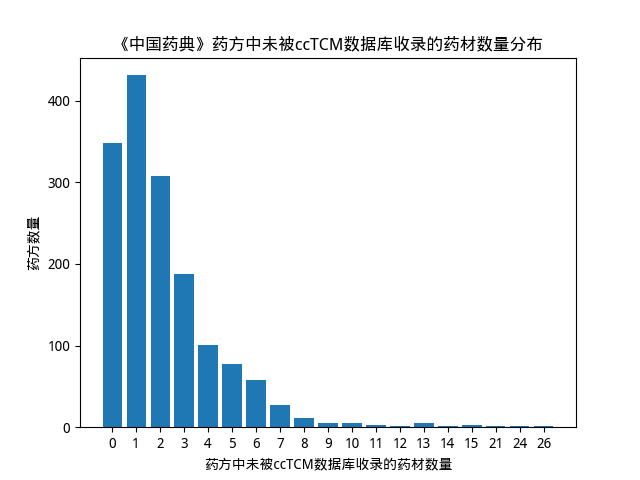
\includegraphics[width=0.8\textwidth]{figures/unlisted_medicinals_distribution.png}
  \caption{《中国药典》中处方在ccTCM中缺失药材数据的分布情况}
  \label{fig:missing_herbs}
\end{figure}

\section{ccTCM 数据库整理}

ccTCM 本身提供了使用中药、化合物或者基因靶标进行在线搜索的平台,但是这种访问方式不利于大规模的数据整理,因此我们选择了直接下载 ccTCM 的原始数据进行离线分析。这些数据以 TSV 格式存储在 {TCM\_information}、{Compound\_information}、{Target\_information} 这些基础信息文件和 {TCM\_compound-v1}、{Compound\_target-v1} 这两层关联文件之中,可以使用数据库合并的逻辑直接得到我们想要的信息,即药材中具体化合物的定量及特定化合物关联各基因的作用强度。其中,化合物定量往往可以给出一个具体的百分比范围,取其平均值进行后续计算即可,但是仅有 42\% 的化合物-基因关联存在以某种形式定量的作用强度,

而且存在量纲不一致、大量作用强度只使用占位值(如 $100000~\mathrm{nM}$ )的问题,几乎没有进行横向比较的可能,在本研究中只能暂时不考虑作用强度问题,或在某种程度上将其视为可学习的参数。我们实际得到的药材-基因定量关联权重是考虑所有与某种基因有关联的化合物,对它们在药材中的占比进行求和的结果,即:


\begin{align}
w_{\text{herb-gene}} = \sum_{\text{compound} \in \text{herb}} w_{\text{herb-compound}} \mathbf{1}_{\text{compound relates to gene}}
\end{align}

这个求和可以在ccTCM表格处理中直接进行,而不需要即时计算,最终我们对每个药材得到并存储一个基因-权重字典应用于后续的基因关联网络构建。

\section{STRING查询与整理}

根据2024年5月31日的数据,STRING 数据库共收录 12535 种生物体的近 6000 万个蛋白质, 互作关系的规模大于 200 亿,是一个非常庞大的数据库,但是其提供了丰富的查询接口,并编写了详细的说明文档(\url{https://string-db.org/help/api/})。在这里,我们希望探究的是药材之前的相互作用,可分解为这样的子问题:遍历处方涉及的药材中的所有二元药材配对,这两个药材关联基因的信息已经在前一步中获得,然后我们将这两个基因列表合并后调用STRING的 {network} API,就可以得到以原始 TSV 或 JSON 格式返回的基因互作分数网络,包括基因近邻分数、融合分数等多项细分关联度和STRING给出的一个综合分数,或者直接给出可视化图像。接下来,我们就可以利用原来的列表从返回的网络中筛选所需的交互关联,以及作为对照的药材内部关联,如下面“二冬膏”的例子:


\begin{figure}[H]
  \centering
  \begin{minipage}[b]{0.4\textwidth}
      \centering
      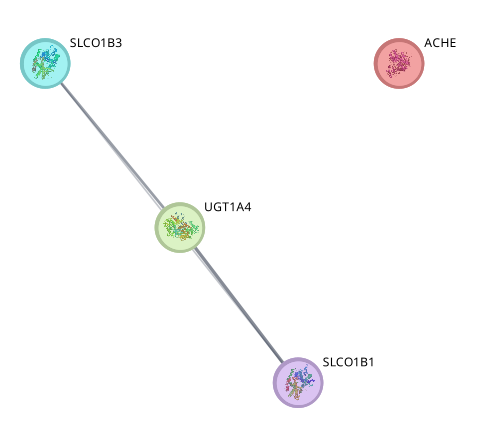
\includegraphics[width=\textwidth]{tiandong.png}
  \end{minipage}
  \hspace{0.05\textwidth}
  \begin{minipage}[b]{0.4\textwidth}
      \centering
      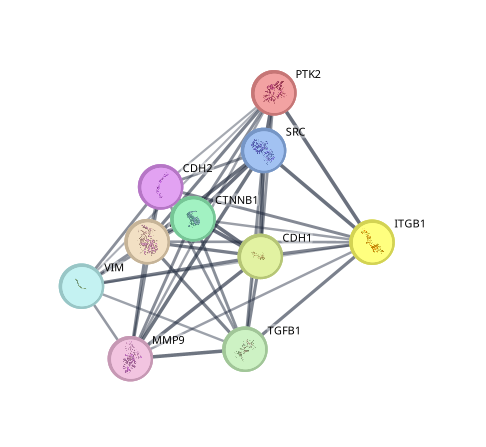
\includegraphics[width=\textwidth]{maidong.png}
  \end{minipage}

  \begin{minipage}[b]{0.95\textwidth}
      \centering
      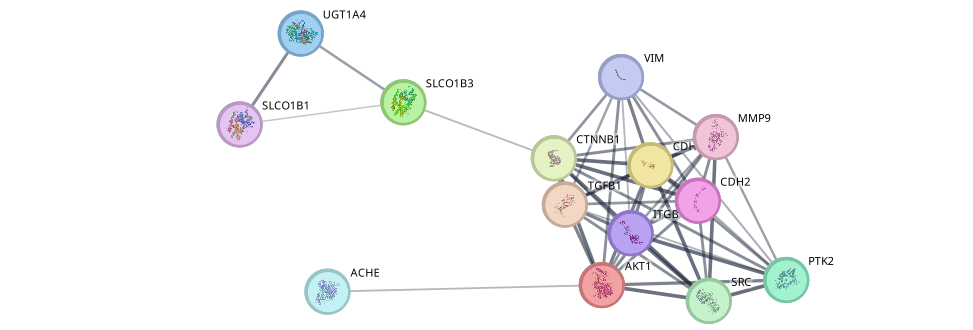
\includegraphics[width=\textwidth]{tiandong-maidong.png}
  \end{minipage}
  \caption{“二冬膏”中药材天冬、麦冬及合并后的基因关联网络示意图}
\end{figure}

“二冬膏”是一个较为简单、只包含两种药材的处方,方便用来作为示例。如果我们分别向STRING的{network} API 发送天冬关联的基因列表(ACHE、UGT1A4、SLCO1B3、SLCO1B1)和麦冬关联的基因列表(CDH1、VIM、CTNNB1、SRC、AKT1、ITGB1、MMP9、TGFB1、PTK2、CDH2)得到的是药材内部的基因关联网络,如左上、右上两图;而将这两个列表合并后发送,得到的是涉及两药材的全基因关联网络,如下图。我们不仅可以根据原来的基因列表筛选出仅发生在两药材之间的关联,还可以将其与药材内部的关联进行对比,或者衡量连通度等关联增益。在这个例子中,天冬关联的4个基因原本被分为不连通的两个部分,但是在与麦冬关联的基因列表合并后,这两个部分被连接了起来,最终的关联图只有一个连通部分,这可能意味着更强的协同作用。

需要注意的是,不同药材的已知关联基因数目可能有极大的差异。上述天冬、麦冬只有10个以内的已知关联基因,而有些药材可能有数千个,以下列出了本研究中已知关联基因较多的几个药材:

\begin{figure}[H]
  \centering
  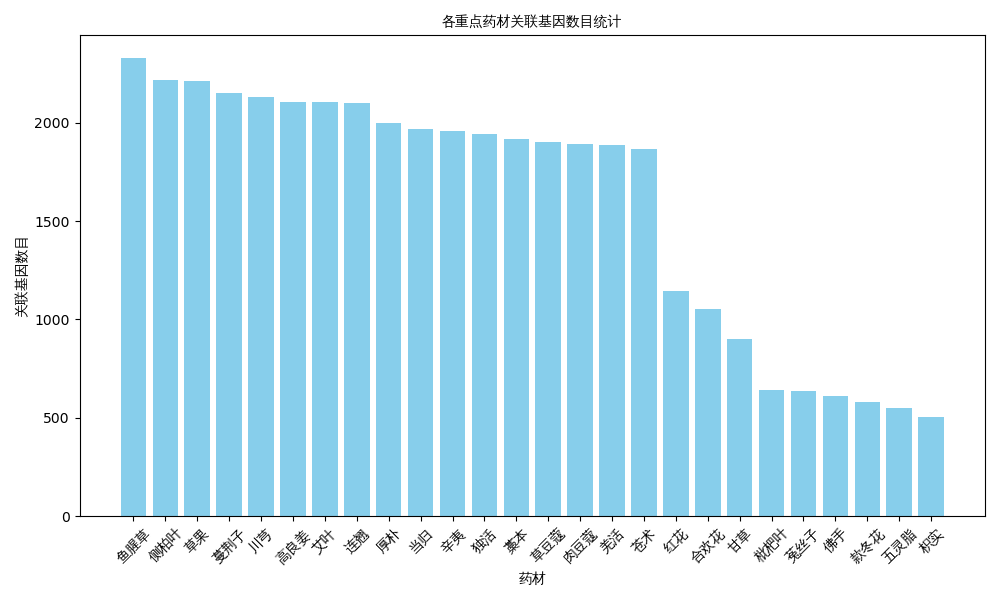
\includegraphics[width=0.8\textwidth]{gene_counts.png}
  \caption{关联基因数大于500的药材及相应基因数}
  \label{fig:top_genes}
\end{figure}

这种关联基因数的不均衡分布不仅会带来后续处理中的一些问题,如关联基因较多的药材可能会自然使得所属网络有显著的关联增益,使得药材始终被认为是“有效的”,或者某些药材关联的基因会完全覆盖其他药材,而且对 API 本身的调用也有影响。经过测试,{network} API所能接受的最大基因数目为2000,而我们的数据中已经有关联超过2000个基因的药材,但由于广泛存在的基因重复,实际任意药材涉及到的总基因数不超过4000,此时就可以采取分组提交的方法克服这一困难。对于任意一个长度不超过4000的基因列表,将其近似均分为4份,记为 a、b、c、d,然后依次提交 ab、ac、ad、bc、bd、cd 这6个列表,最后再将返回的网络合并即可。

如果仅仅进行现有药方的分析,我们只需要对各个药方中真实存在的药材配对进行查询。但是,我们在后续比较中可能需要足够的负例,即并不真实存在、大概率无临床价值的随机药物组合。这大约是7.2倍的查询量,即从真实处方中出现的1685个药材配对扩展到全部$\frac{1}{2} \times 156 \times (156 - 1) = 12090$种可能。

需要注意的是,虽然STRING支持使用 Uniprot ID, NCBI Gene ID和自建的STRING ID进行查询,但是 {network} API的返回结果中仅有 STRING ID和NCBI Gene ID,但ccTCM提供的是Uniprot ID,这导致数据反查时遇到困难。同时,STRING数据库未收录ccTCM中的部分基因。为此,我们借助STRING的 {get\_string\_ids} API得到这三种基因表示间的对应关系,在本地建立相应的映射表,并从药材关联的基因中除去未被STRING收录的部分。
% !TeX root = ../thuthesis-example.tex

\chapter{模型建立与应用}

\section{使用药材配对直接分析处方效果的尝试}

在引入更复杂的模型前,一个自然的想法是探究参与构成有效处方和不参与的药材配对在基因关联强度上是否有显著差异。如果这种假设成立,我们便可以直接通过评价药方中药材配对的好坏来分析其有效性。

\subsection{基于基因关联图连通部分减少数的分析}

我们可以沿用之前分析处方“二冬膏”时使用图的连通度的方法,批量地考察药材配对后是否能够显著减少基因关联图的连通部分数。如果出现这种情况,说明这两种药材联合使用可能共同作用于某些生物通路,起到互补的作用。可以对处方药材配对和随机药材配对作出如下的分布图进行对比:

\begin{figure}[H]
  \centering
  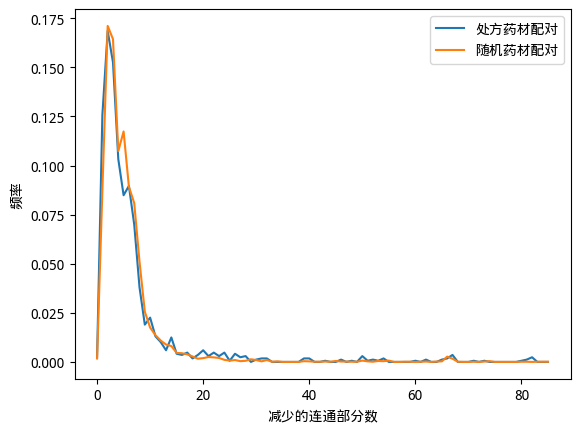
\includegraphics[width=\linewidth]{component_reduction_pdf.png}
  \caption{处方和随机药材配对减少的基因关联图连通部分数分布}
  \label{fig:component_reduction_pdf}
\end{figure}

\begin{figure}[H]
  \centering
  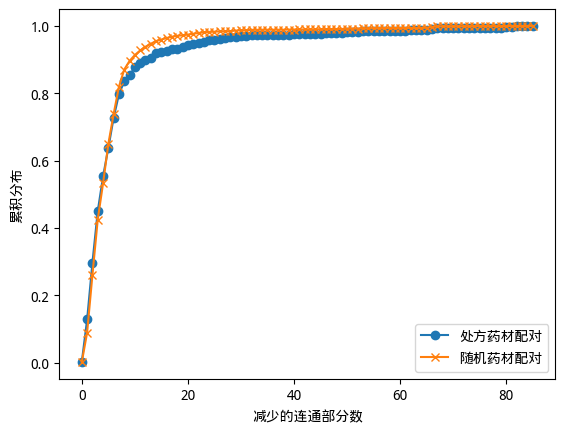
\includegraphics[width=\linewidth]{component_reduction_cdf.png}
  \caption{处方和随机药材配对减少的基因关联图连通部分数累积分布}
  \label{fig:component_reduction_cdf}
\end{figure}

此时双样本Kolmogorov-Smirnov检验的$D$值为$0.0409$,$p$值为$0.015$,可以得到显著差异,说明处方中已有的药材配对倾向于更多地减少基因关联图中的连通部分,这可能是药材配对的有效性的一个重要特征。

\subsection{基于网络分数增益的分析}


为了应用定量信息,我们可以考察药材配对之间增加的关联边数或者边权重之和,然后将真实的药材配对和所有可能药材配对分别进行排序,作出增益-分位数曲线,从而比较“是否属于已知处方”能否带来统计差异。同时,我们也可以尝试使用基因在药材中通过化合物的定量信息,观察增加这个额外信息相比仅使用STRING给出的分数是否能给出更显著的统计差异。下图是在应用与不应用化合物定量信息的条件下作出的对比曲线:

\begin{figure}[H]
  \centering
  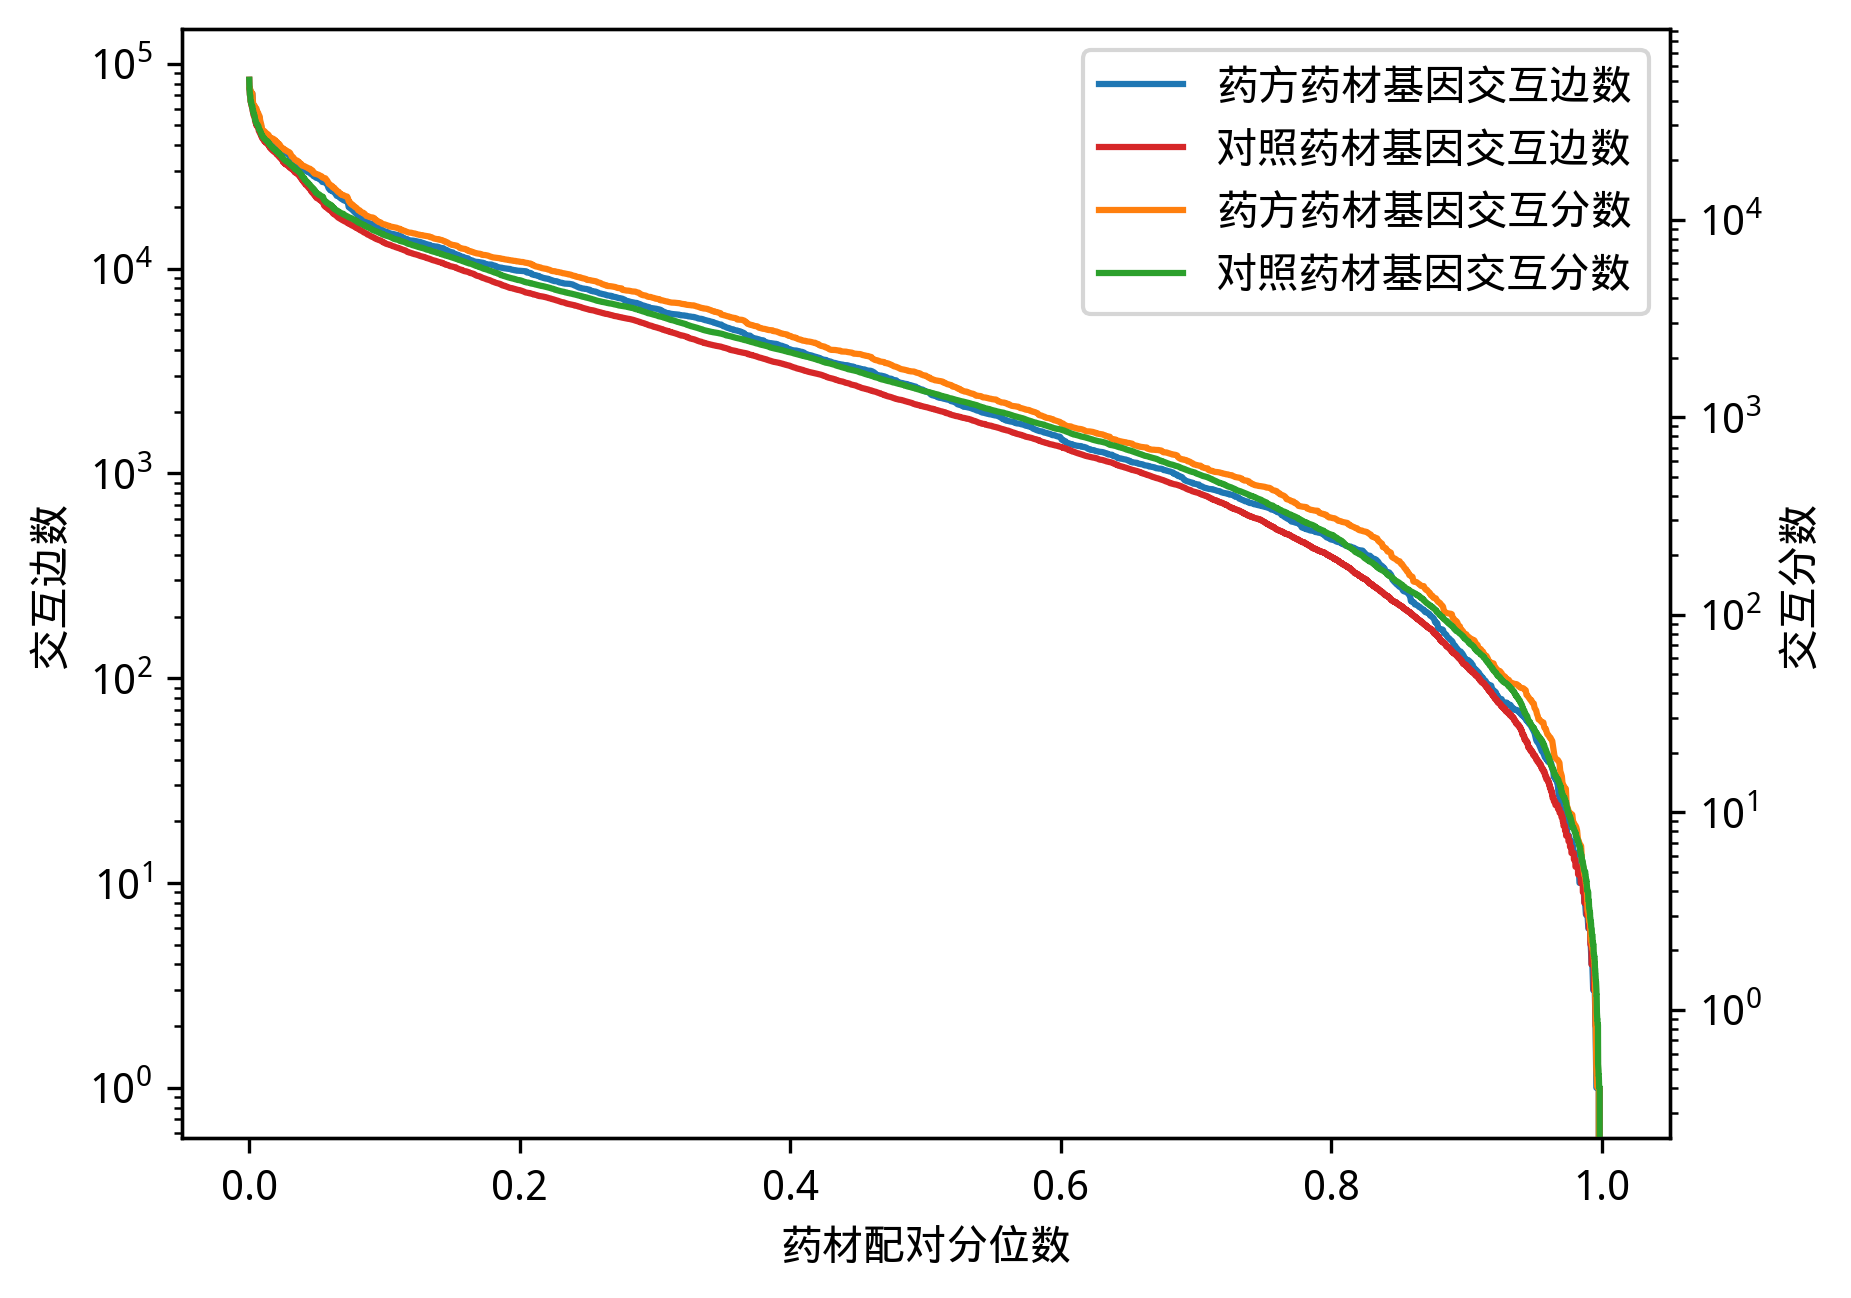
\includegraphics[width=0.95\linewidth]{scores_without_weight.png}
  \caption{不使用化合物定量的药材配对边数/分数增益-分位数曲线}
  \label{fig:score_without_weight}
\end{figure}

\begin{figure}[H]
  \centering
  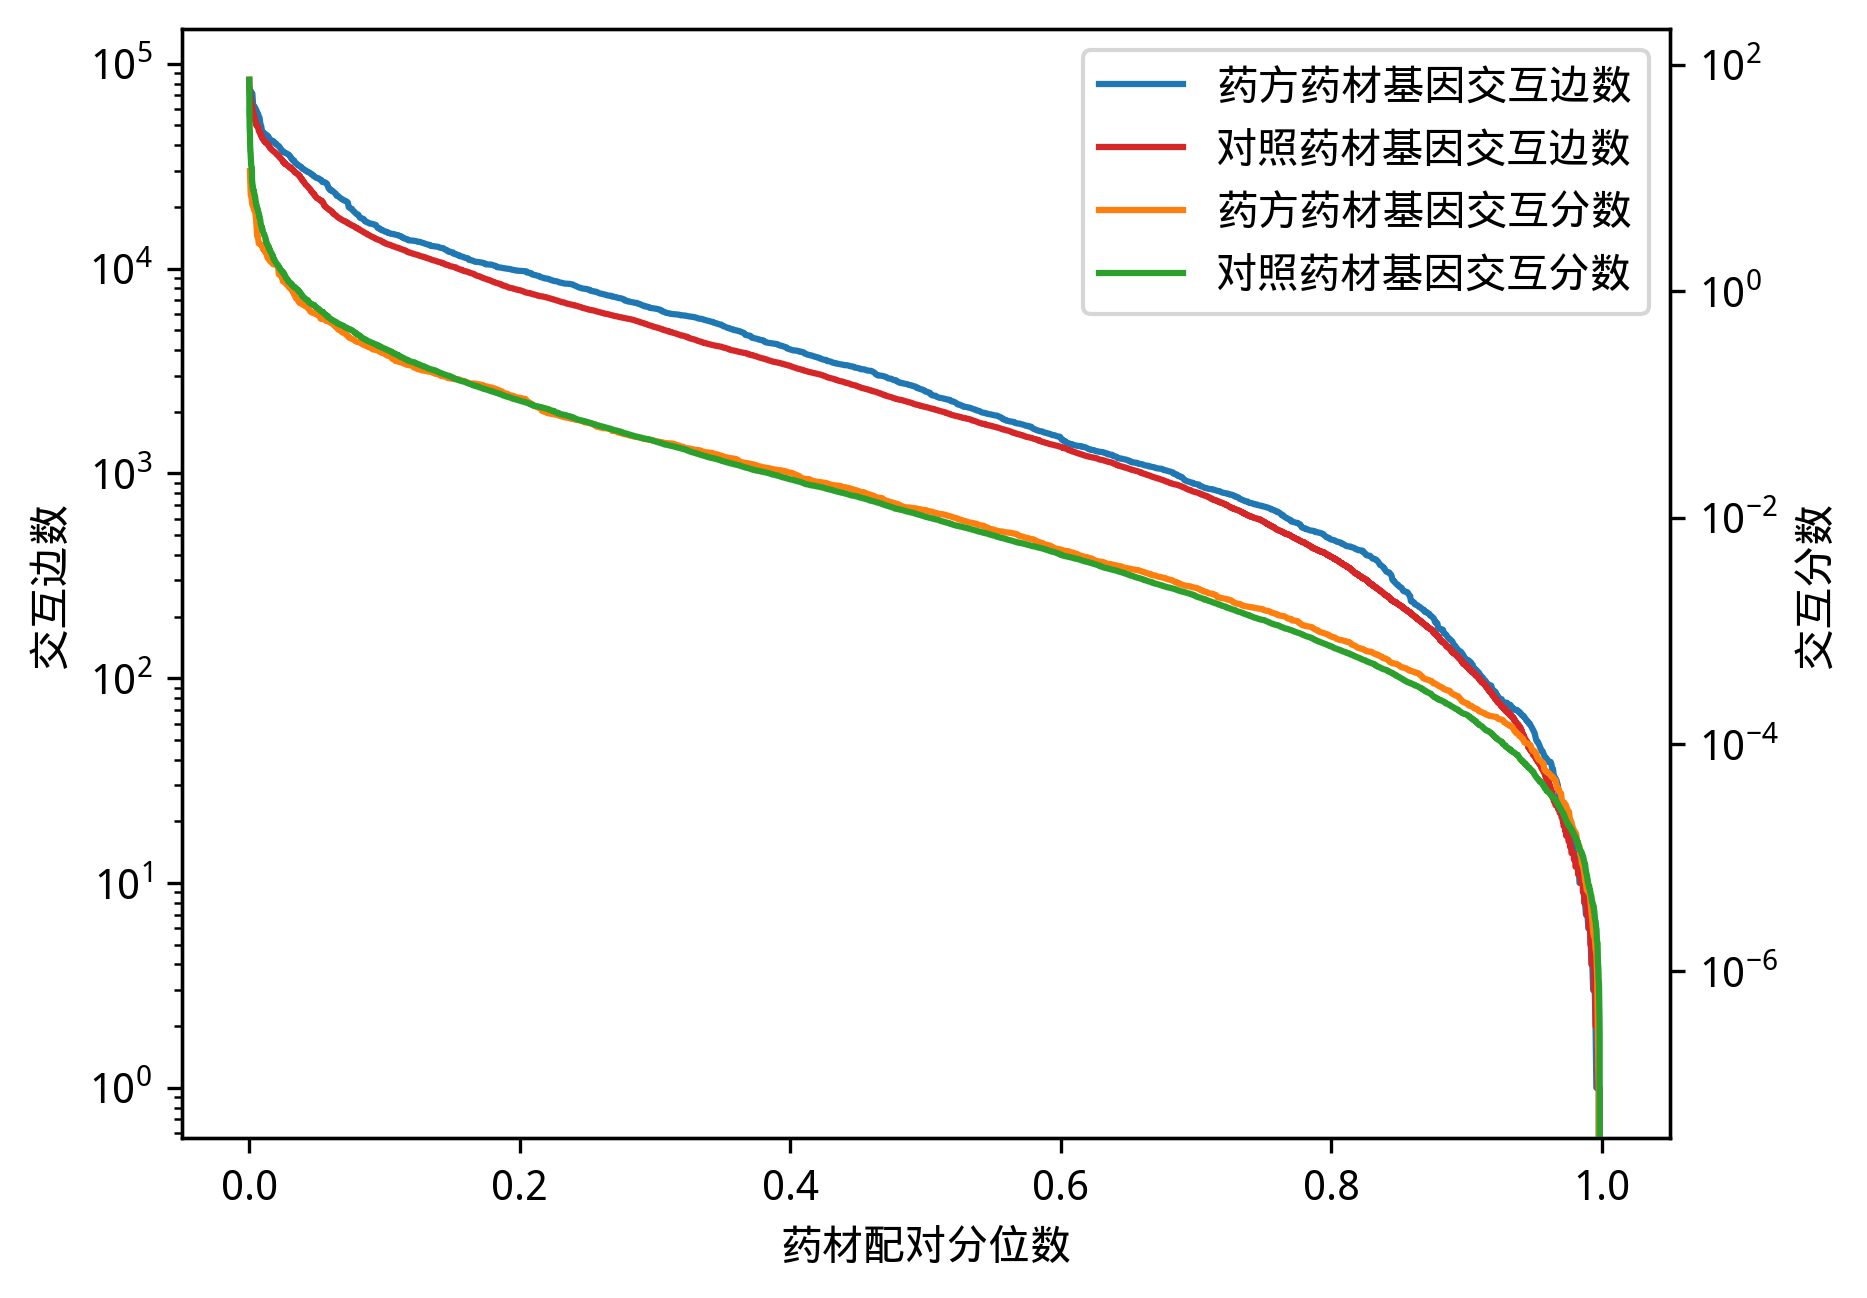
\includegraphics[width=0.95\linewidth]{scores_with_weight.png}
  \caption{使用化合物定量的药材配对边数/分数增益-分位数曲线}
  \label{fig:scores_with_weight}
\end{figure}


虽然我们无法简单地通过边数或分数增益准确地判断药材配对的有效性,但是我们可以从图线中直观地看到,如果不应用化合物定量信息,属于已知处方的药材配对在边数和分数上,几乎各个分位数点处都有优势。使用双样本Kolmogorov-Smirnov检验,可以得到边数的$D$值为$0.0551$,$p$值为$0.00029$,分数的$D$值为$0.05556$,$p$值为$0.00024$,即这两种指标均能说明是否属于已知药方会导致显著差异,而引入STRING关联分数可以略微提升置信度。

然而,当我们在此引入化合物含量信息后,从图线上发现,增益曲线的差异性几乎消失,甚至有明显的反转区域;双样本Kolmogorov-Smirnov检验的$D$值为$0.0243$,$p$值为$0.35$,无法得到显著差异,这说明化合物含量信息的引入反而使得药材配对的边数和分数增益失去了区分性。这可能是因为化合物含量信息本身存在大量数量级层面的差异,直接相乘引入了过大的噪声。

为了解决上面的问题,我们考虑使用对化合物含量进行归一化,即使用 $\frac{(w_{a1}+w_{a2})(w_{b_1}+w_{b2})}{w_{a1}w_{b2}+w_{b1}w_{a2}}$来作为 1,2 两个药材中基因对 $(a, b)$ 的化合物定量权重。这样,我们可以得到如下的增益曲线:

\begin{figure}[H]
  \centering
  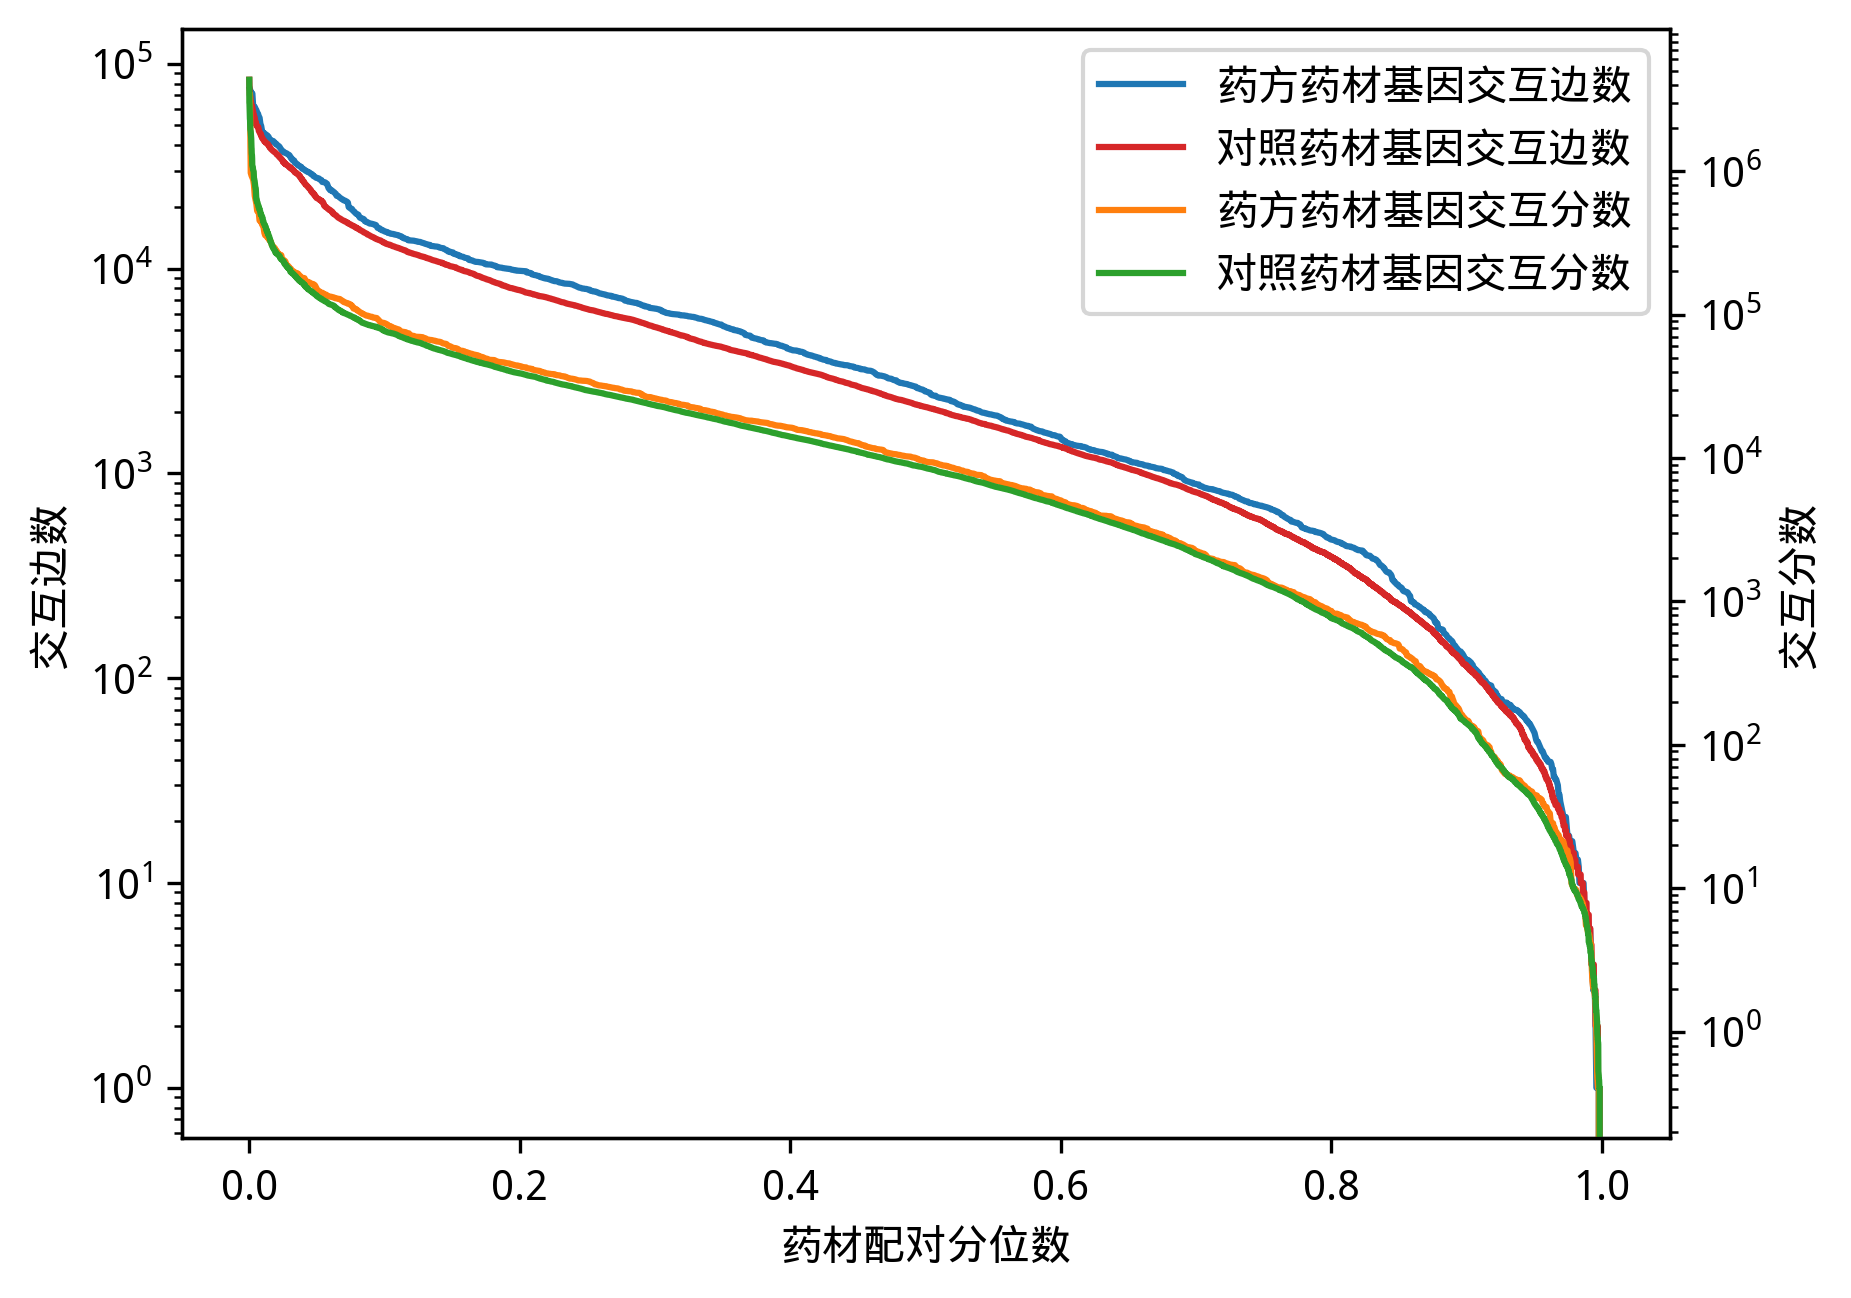
\includegraphics[width=0.95\linewidth]{scores_with_normalized_weight.png}
  \caption{使用归一化化合物定量的药材配对边数/分数增益-分位数曲线}
  \label{fig:scores_with_normalized_weight}
\end{figure}

这里的图线相比之前得到了改善,可以观察出药方药材配对几乎始终在对照药材配对上方,但双样本Kolmogorov-Smirnov检验具有$D$值为$0.0314$,$p$值为$0.11$,仍然没有显著性,说明对数在此问题中可能是一个更好的转换方式。但定量信息依然没有为药材配对的边数和分数增益带来提升,说明我们可能还需要建立更复杂的模型来运用定量信息解释处方的效果。

% edge
% KstestResult(statistic=0.05506882248177303, pvalue=0.0002908647549561178, statistic_location=5799, statistic_sign=-1)
% unweighted
% KstestResult(statistic=0.05564546832511763, pvalue=0.00024155665548500303, statistic_location=3674.2729999999983, statistic_sign=-1)
% weighted
% KstestResult(statistic=0.024379685069236018, pvalue=0.34918573567118794, statistic_location=0.0013520617904999987, statistic_sign=-1)
% normalized
% KstestResult(statistic=0.031446876287792414, pvalue=0.11124597693644322, statistic_location=13623.52746273345, statistic_sign=-1)

\section{使用图神经网络的处方效果预测}

如果从处方层面考虑问题,我们可以作出这样的假设:各基因受处方整体的作用等于处方中各药材影响的代数和,来自不同药材或不同化合物的基因影响在混同后是完全等价的。在这种假设下,我们可以直接遍历处方中的每个药材求和,得到每个基因的总表达影响,这样就把一个处方建模成了一系列以基因作为顶点,从化合物含量信息推出的总表达影响为点权重,基因之间的关联为边,STRING分数为边权重的图。

然后,利用图神经网络的方法,我们便可以训练模型对处方的效果进行预测,其中设《中国药典》中已经存在的处方为正例,而随机生成的、大概率不会有现实药理作用的处方为负例,便形成了一个通过图特征进行二分类的问题。这事实上是一个正无标签学习问题,我们没有确信的负例,即通过实验验证不存在任何正向药理作用的处方。这种情况下,由于正例是固定的,数量上非常有限,而负例可以通过从药材列表中任意选择,随机赋予定量,几乎无限地生成。相比于构造平衡的处方数据集,如果采样更多负例,即虚拟处方来训练,可能更有利于发现正例特有的特征。但是,这也会使得原有的准确率、召回率无法直接反映处方判别模型性能,需要使用采样、加权的方法克服这些问题。在本研究中,我们采用的是构建均衡样本的方法,但是模型实际调优时依然可以使用不均衡的策略。

在实际的训练和预测过程中,图的节点数,即处方中的药材数,会显著影响连接密度和图表示,是重要的特征,但有效处方的实际大小存在显著的区别,其中大小在8及以下的处方出现的频次较多。这一方面和指导处方配伍的中医传统理论有关,另一方面一个显著的影响因素是药材的定量信息不足,越大的处方越容易出现缺少药材定量而无法入选有效处方的情况。对比不考虑处方完整性的原始处方大小,我们可以发现其中不乏大于20味药材的处方,而不是到16即止,但这些都无法在现有的数据下得到体现。完整、可利用处方具体的大小分布如下:

% 此处存在较多留白,需要补充

\begin{figure}[H]
  \centering
  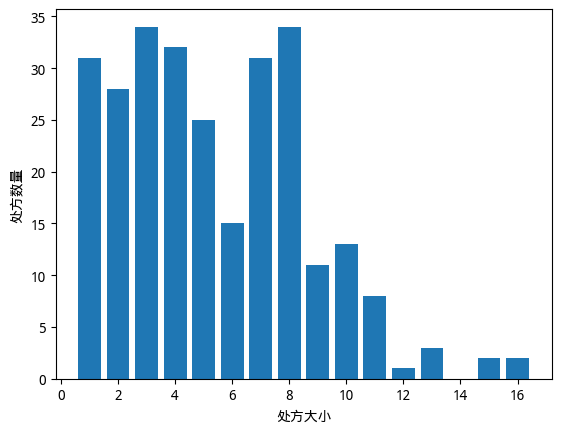
\includegraphics[width=\linewidth]{prescription_size.png}
  \caption{《中国药典》中药材均在ccTCM中收录的处方大小分布}
  \label{fig:prescription_size}
\end{figure}

为了防止学习到的实际上是有效处方较可能拥有的大小而非底层的关联信息,我们不能简单地随机指定生成虚拟药方的大小,而要使生成集合中各大小的处方比例也与《中国药典》中的已知处方相近。然而,从上述分布图中,我们可以看出处方大小9开始有一次显著的下降,而大小在12及以上的处方每个大小仅有0-3个已知记录。如果直接进行训练-验证-测试集的划分,将极有可能出现不均衡的现象,即较大而稀少的处方出现在训练和测试中的比例差别大,从而影响构造的类似大小负例的判别。因此,我们可以初步尝试直接去掉这些较大的处方,提高模型的稳定性,但更好的方法应是通过一定的采样策略来平衡数据集,比较建模效果,判断这些较大的处方样本是否含有标签推断中的重要信息。

另一方面,涉及药材非常少的较小处方也值得我们关注。这其中的一个特例是只含有一味药材的处方,即《中国药典》中分类的“单味制剂”,由于处方中药材的用量需要归一化,单味制剂药材权重始终为1,如果我们在随机构造中选取与现有单味制剂所用药材相同的药材,结果将与现有处方完全相同,将为正例而无标签例,在此这种情况出现的可能性显著高于规模更大的处方,因此需要特殊处理。除了这个较为显然的影响外,还有一种不容忽视的情况是较小的处方可能作为其他处方的子图存在。在这种情况下,一方面我们基于临床经验往往得以判定额外的药材至少不会对处方产生负面影响,即新的更大的处方应仍然是有效的;另一方面,这种有效性往往很难证明来自网络扩大后引入其他药材的影响,除非它们的实际生理药理作用有显著的不同,但这种不同在现有的,未结合临床征候的数据中没有得到体现。在这里,本研究的倾向是不考虑以有效子图为基础的扩大处方因此而获得的有效性,而关注其自身的特征,至少在模型学习的阶段不引入这个先验。这是因为建模的目标是发现构成有效药方的不同的基础特征,而不是单纯求取更好的预测性能。从临床实践的观点上看,这种策略有助于我们发现新的简单基础的有效药方,而不是扩大已有的处方,以数量取胜。

\subsection{基于图卷积网络的分析}

我们首先考虑了朴素的图卷积网络(GCN),它使用简单的层次化方法聚合节点的邻域信息,适合于这里的基因表达关联。应用GCN模型对处方是否真实存在的标签进行预测,实验环境的具体配置如下:


\begin{table}
  \centering
  \caption{实验环境配置}
  \begin{tabular}{ll}
    \toprule
    操作系统             & CentOS 7.5.1804                           \\
    CPU              & Intel(R) Xeon(R) Gold 6226R CPU @ 2.90GHz \\
    GPU              & Tesla V100-SXM2-32GB                      \\
    CUDA             & 11.4                                      \\
    cuDNN            & 7.5.1                                     \\
    Python           & 3.10.0                                    \\
    PyTorch          & 1.12.1                                    \\
    torch\_geometric & 2.5.3                                     \\
    scikit-learn     & 1.3.2                                     \\
    \bottomrule
  \end{tabular}
  \label{tab:three-line}
\end{table}

可在单卡上对此数据集进行常规规模的学习,得到的训练和测试曲线如下:

% 此处存在较多留白,需要补充

\begin{figure}[H]
  \centering
  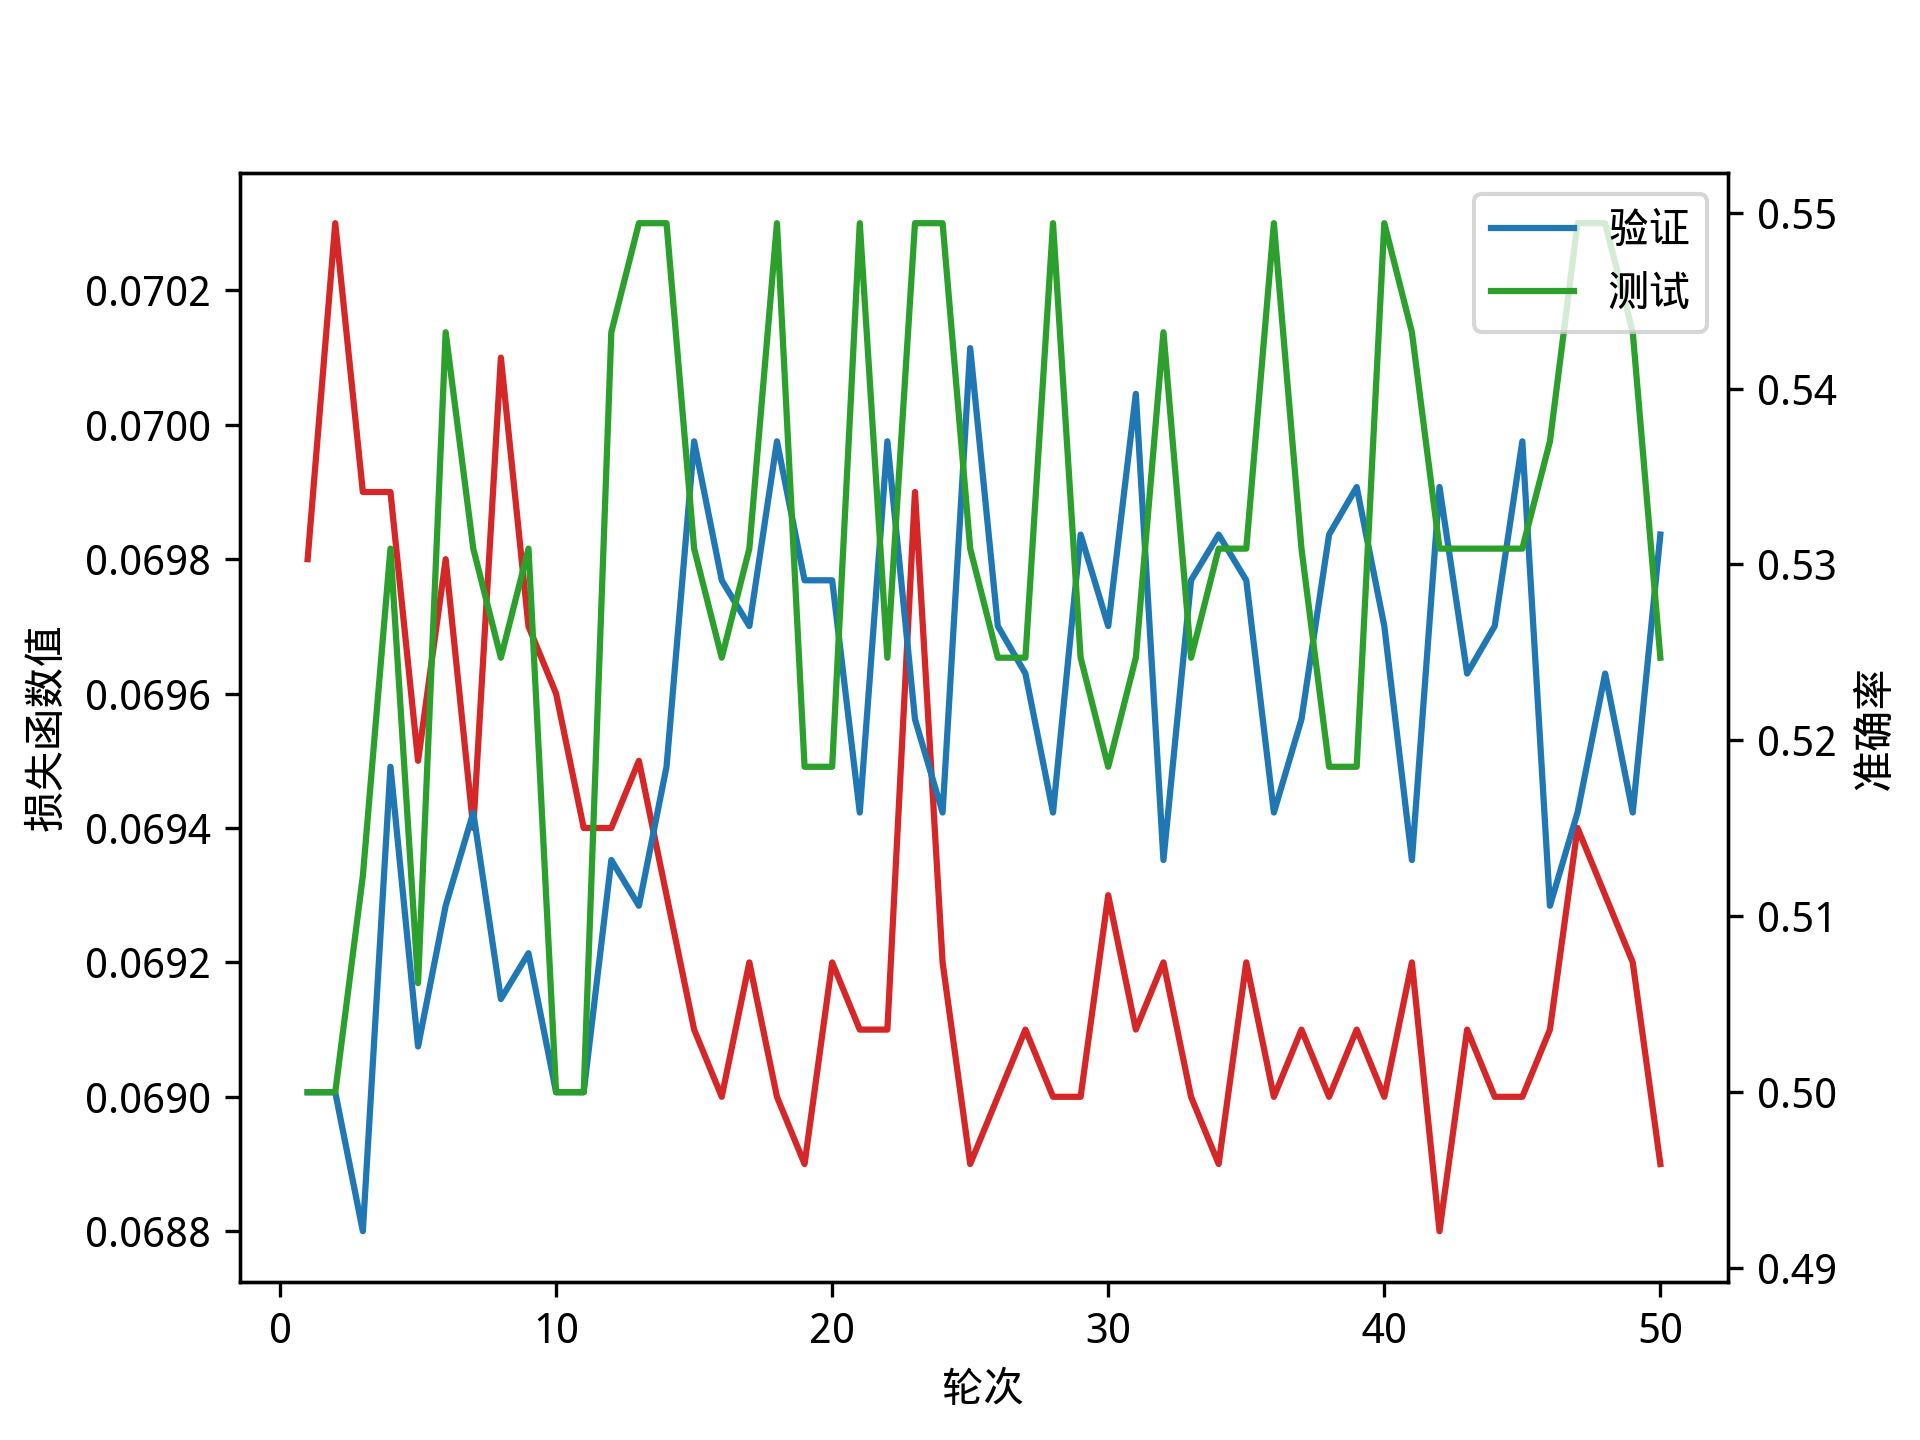
\includegraphics[width=\linewidth]{gcn_0.01.png}
  \caption{GCN模型的训练和测试曲线}
  \label{fig:gcn_train_curve}
\end{figure}

可能是由于化合物定量信息表征能力有限,或者没有选取更优的模型进行学习,得到的模型预测准确率的提升并不高,但至少稳定在0.5以上,均值达到0.53左右,至少说明了一定的预测能力。验证集和测试集上的处方标签预测正确率均处在比较低的水平上,大概率显示模型存在表征能力不足、欠拟合的问题。在这种情况下,我们可以考虑使用更适于表征学习的模型,如自编码器(autoencoder, AE)。

\subsection{基于自编码器的分析}

自编码器是一种主要为了将输入编码为压缩的、有意义的表示,然后重新解码,使得结果与最初输入尽可能接近,以学习无标签数据的抽象特征的神经网络,\cite{Bank_Koenigstein_Giryes_2021},最早由Rumelhart、Hinton和Williams等人在1986年提出\cite{10.5555/104279.104293}。在本研究中,我们首先定义了一个简单的图自动编码器,使用GCN层进行编码,全连接层进行解码,从而提取和重构处方的特征。在训练过程中,我们仅使用正例数据,直至逐元素的最小均方误差损失收敛。对于使用化合物含量信息作为节点权重的自编码器,在50个训练周期后收敛到 $3\times 10^{-5}$ 左右。


然后,我们提取图的低维表示。自编码器后可接不同的分类器,故我们选取了诸多经典的机器学习算法,包括逻辑回归、支持向量机、随机森林、梯度提升、AdaBoost、多层感知机、高斯朴素贝叶斯、K近邻,分别进行分类预测,并输出相应的分类报告,以进行分类器准确率、对处方正负例及加权平均意义下的精确率、召回率、F1分数等预测性能指标的比较。具体的实验结果如下:

\begin{table}[H]
  \centering
  \resizebox{\textwidth}{!}{%
    \begin{tabular}{lccccccccccc}
      \toprule
      \multirow{2}{*}{模型} & \multirow{2}{*}{准确率} & \multirow{2}{*}{AUC} & \multicolumn{3}{c}{正例} & \multicolumn{3}{c}{负例} & \multicolumn{3}{c}{加权平均}                                           \\
                          &                      &                      & 精确率                     & 召回率                     & F1                        & 精确率  & 召回率  & F1   & 精确率  & 召回率  & F1   \\
      \midrule
      逻辑回归                & 0.568                & 0.600                & 0.55                    & 0.75                    & 0.63                      & 0.62 & 0.39 & 0.48 & 0.58 & 0.57 & 0.55 \\
      支持向量机               & 0.562                & 0.371                & 0.53                    & 0.91                    & 0.67                      & 0.72 & 0.22 & 0.34 & 0.63 & 0.56 & 0.50 \\
      随机森林                & 0.716                & 0.725                & 0.69                    & 0.78                    & 0.73                      & 0.75 & 0.66 & 0.70 & 0.72 & 0.72 & 0.72 \\
      梯度提升                & 0.654                & 0.710                & 0.65                    & 0.64                    & 0.65                      & 0.65 & 0.67 & 0.66 & 0.65 & 0.65 & 0.65 \\
      AdaBoost            & 0.586                & 0.585                & 0.63                    & 0.40                    & 0.49                      & 0.57 & 0.77 & 0.65 & 0.60 & 0.58 & 0.57 \\
      多层感知机               & 0.531                & 0.511                & 0.51                    & 0.89                    & 0.65                      & 0.62 & 0.18 & 0.28 & 0.57 & 0.54 & 0.47 \\
      朴素贝叶斯               & 0.494                & 0.529                & 0.49                    & 0.94                    & 0.65                      & 0.50 & 0.06 & 0.11 & 0.50 & 0.50 & 0.38 \\
      K近邻                 & 0.617                & 0.636                & 0.60                    & 0.65                    & 0.63                      & 0.63 & 0.59 & 0.61 & 0.62 & 0.62 & 0.62 \\
      \bottomrule
    \end{tabular}
  }
  \caption{应用化合物定量信息和基因关联的自编码器各分类器性能对比}
  \label{tab:performance_comparison}
\end{table}

可以看出,在参与比较的分类器中,随机森林取得了最高的准确率、AUC和加权平均F1分数,分别达到了0.716,0.725和0.72,显示出了较强的分类能力。使用这个模型,我们将可能区分一个新处方是否具有与成方相似的底层特征,从而对其有效性进行一定推断。为了判断化合物含量是否有助于提升模型预测准确率,我们在代码中进行相对应的修改,不再使用权重信息,即将每个关联边的点权重都设置为1。由于节点权重的数量级不同,在50个训练周期后,自编码器的损失函数收敛到 $0.04$ 左右。可以作出两组的训练曲线。

\begin{figure}[htbp]
  \centering
  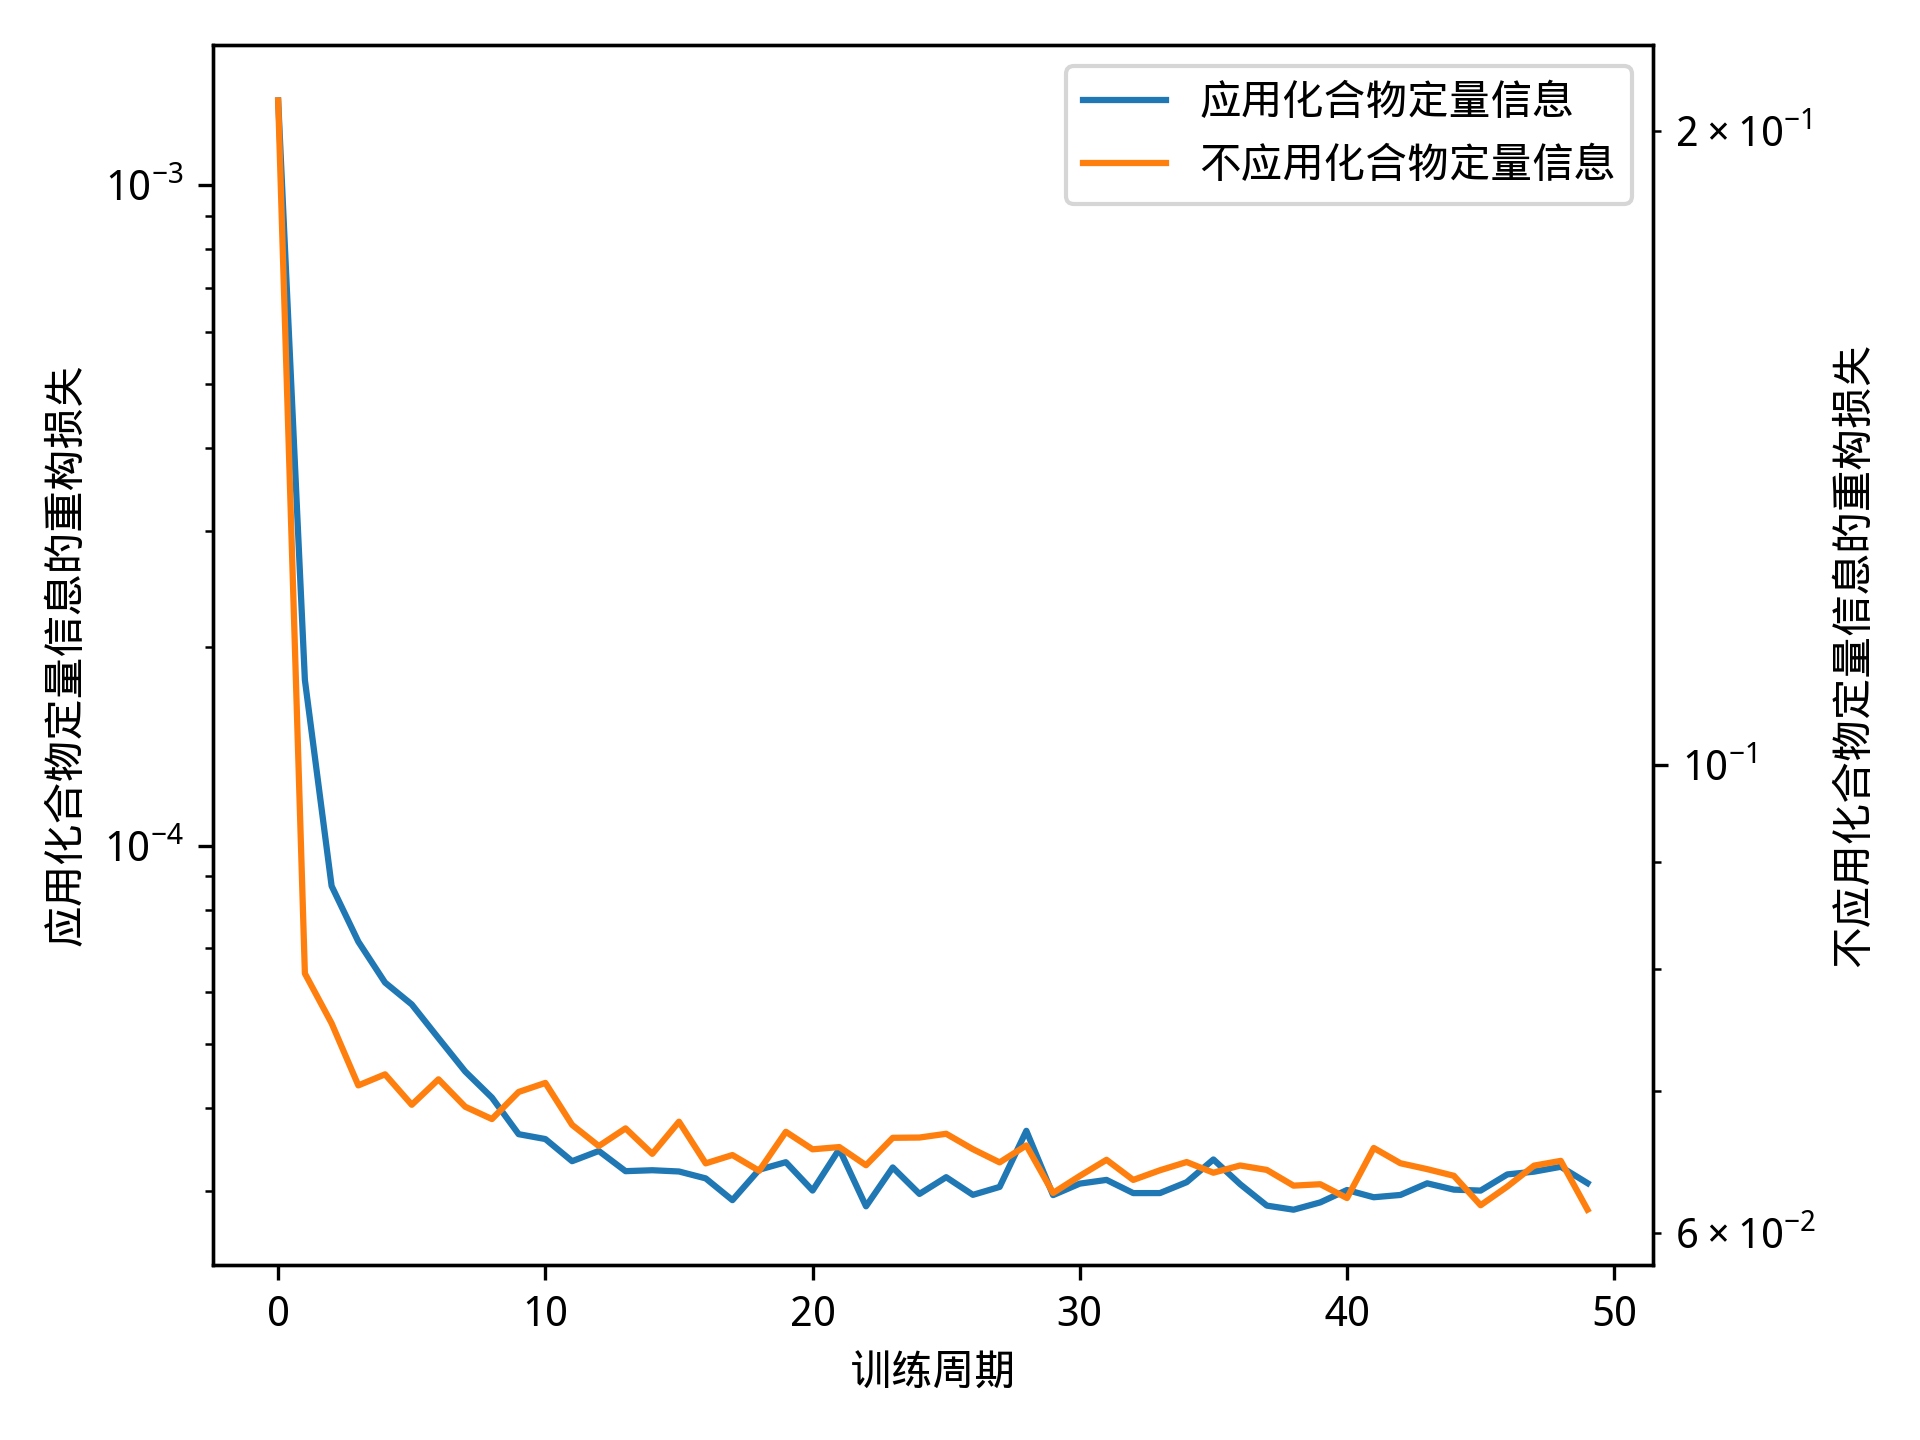
\includegraphics[width=\linewidth]{training_curve.png}
  \caption{使用和不使用化合物定量信息的自编码器训练曲线}
  \label{fig:ae_train_curve}
\end{figure}

可以看到,虽然具体的数值无法直接比较,但两组均达成了收敛。然后,我们在无化合物含量信息的模型上同样使用各种分类器进行预测,得到相应的预测效果。

\begin{table}[H]
  \centering
  \resizebox{\textwidth}{!}{%
    \begin{tabular}{lccccccccccc}
      \toprule
      \multirow{2}{*}{模型} & \multirow{2}{*}{准确率} & \multirow{2}{*}{AUC} & \multicolumn{3}{c}{正例} & \multicolumn{3}{c}{负例} & \multicolumn{3}{c}{加权平均}                                           \\
                          &                      &                      & 精确率                     & 召回率                     & F1                        & 精确率  & 召回率  & F1   & 精确率  & 召回率  & F1   \\
      \midrule
      逻辑回归                & 0.457                & 0.436                & 0.00                    & 0.00                    & 0.00                      & 0.46 & 0.98 & 0.63 & 0.21 & 0.46 & 0.29 \\
      支持向量机               & 0.457                & 0.439                & 0.49                    & 0.34                    & 0.40                      & 0.44 & 0.59 & 0.50 & 0.47 & 0.46 & 0.45 \\
      随机森林                & 0.638                & 0.618                & 0.66                    & 0.66                    & 0.66                      & 0.61 & 0.61 & 0.61 & 0.64 & 0.64 & 0.64 \\
      梯度提升                & 0.572                & 0.579                & 0.59                    & 0.65                    & 0.62                      & 0.54 & 0.48 & 0.51 & 0.57 & 0.57 & 0.57 \\
      AdaBoost            & 0.486                & 0.503                & 0.52                    & 0.47                    & 0.50                      & 0.45 & 0.50 & 0.47 & 0.49 & 0.49 & 0.49 \\
      多层感知机               & 0.486                & 0.453                & 0.53                    & 0.38                    & 0.44                      & 0.46 & 0.61 & 0.52 & 0.50 & 0.49 & 0.48 \\
      朴素贝叶斯               & 0.449                & 0.450                & 0.49                    & 0.53                    & 0.51                      & 0.40 & 0.36 & 0.38 & 0.45 & 0.45 & 0.45 \\
      K近邻                 & 0.522                & 0.549                & 0.56                    & 0.54                    & 0.55                      & 0.48 & 0.50 & 0.49 & 0.52 & 0.52 & 0.52 \\
      \bottomrule
    \end{tabular}
  }
  \caption{只应用基因关联的自编码器各分类器性能对比}
  \label{tab:unweighted_performance_comparison}
\end{table}

直接观察两表,可以看出在大部分分类器和评价指标中,使用化合物定量信息的自编码器的性能要优于不使用的情况,随机森林依然是表现最好的分类器,而在这个分类器上,每一项评价指标的数值均有提升,这说明化合物含量信息的引入对于模型的性能有一定的提升作用。对于以下讨论的其他处理下的分类问题,也具有类似的明显分别,不使用化合物信息的模型性能普遍较差,不再展示相关的实验结果。

之前讨论过,一方面处方过大可能导致在训练集和测试集中的随机分类出现不均衡,但另一方面这些较大的基因关联网络又可能提供更多的基因关联信息,故我们也使用自编码器和不同的分类器来决定是否应该去掉这些较大的处方。在这里,我们将训练集和验证集的处方大小均限制在8及以下,得到的结果如下:

\begin{table}[htbp]
  \centering
  \resizebox{\textwidth}{!}{%
    \begin{tabular}{lccccccccccc}
      \toprule
      \multirow{2}{*}{模型} & \multirow{2}{*}{准确率} & \multirow{2}{*}{AUC} & \multicolumn{3}{c}{正例} & \multicolumn{3}{c}{负例} & \multicolumn{3}{c}{加权平均}                                           \\
                          &                      &                      & 精确率                     & 召回率                     & F1                        & 精确率  & 召回率  & F1   & 精确率  & 召回率  & F1   \\
      \midrule
      逻辑回归                & 0.522                & 0.546                & 0.53                    & 0.70                    & 0.60                      & 0.51 & 0.33 & 0.40 & 0.52 & 0.52 & 0.50 \\
      支持向量机               & 0.457                & 0.530                & 0.43                    & 0.18                    & 0.26                      & 0.46 & 0.75 & 0.57 & 0.45 & 0.46 & 0.41 \\
      随机森林                & 0.572                & 0.615                & 0.58                    & 0.61                    & 0.59                      & 0.56 & 0.54 & 0.55 & 0.57 & 0.57 & 0.57 \\
      梯度提升                & 0.558                & 0.606                & 0.58                    & 0.49                    & 0.53                      & 0.54 & 0.63 & 0.58 & 0.56 & 0.56 & 0.56 \\
      AdaBoost            & 0.543                & 0.559                & 0.59                    & 0.38                    & 0.46                      & 0.52 & 0.72 & 0.60 & 0.55 & 0.54 & 0.53 \\
      多层感知机               & 0.486                & 0.480                & 0.50                    & 0.72                    & 0.59                      & 0.44 & 0.24 & 0.31 & 0.47 & 0.49 & 0.45 \\
      朴素贝叶斯               & 0.514                & 0.500                & 0.52                    & 0.90                    & 0.66                      & 0.50 & 0.10 & 0.17 & 0.51 & 0.51 & 0.42 \\
      K近邻                 & 0.493                & 0.567                & 0.51                    & 0.59                    & 0.55                      & 0.47 & 0.39 & 0.43 & 0.49 & 0.49 & 0.49 \\
      \bottomrule
    \end{tabular}
  }
  \caption{去除大于等于9种药材的处方后自编码器各分类器性能对比}
  \label{tab:reduced_performance_comparison}
\end{table}

从准确率的角度而言,去除较大的处方后,分类器的也均性能下降。性能最高的随机森林分类器性能下降显著。需要注意的是,这还仅为在处方大小为8及以下的情况下的结果,而更大的真实处方还完全没有引入到评测,相应的特征是未学习的。因此,总体而言,尽管去除较大的处方可能有助于数据集的稳定性,但是在实际的预测中,这些处方可能仍然具有重要的信息,去除后会导致模型性能的下降。
    % !TeX root = ../thuthesis-example.tex

\chapter{总结和展望}

\section{总结}

本研究的工作主要可以归结为数据收集和建模分析两个部分。其中,在数据收集方面,主要对《中国药典》、ccTCM项目原始数据、STRING蛋白互作数据库中和中药化合物有关的基因及其表达关联进行了获取和整理,不仅用于项目本身,也为后续应用其他分析方法提供了基础,如《中国药典》的格式化文本可用于提取中药处方标准各方面的信息;在建模分析方面,我们尝试了对药材配对直接进行作图比较和双样本Kolmogorov-Smirnov非参数检验方法,虽然初步得出了在药材基因交互边数和分数的定量标准下,已知有效处方和随机构造的虚拟处方在总体上有显著差异,从一个侧面反映了处方的有效性可能被网络关系描述,但没有得到直接判断药材配对是否有利于形成有效处方的标准,然后我们尝试了基于图神经网络的方法,通过对药材配对的图结构进行学习,得到了一定的预测效果,对于正负例均衡的样本使用自编码器和随机森林分类器,得到最高0.716的准确率,0.725的AUC和0.72的加权平均F1分数,并验证了使用化合物定量信息可以提高模型训练的有效性,普遍提升预测性能指标,说明在中药处方评估和靶点预测问题中应用定量信息是有帮助的。但是,由于数据量和模型复杂性的限制,预测准确率仍有待进一步提高。

\section{展望}

现阶段,《中国药典》中部分处方定量信息并没有具体提供,或者形式上不够直观可用;ccTCM等中药化合物定量数据库不够完善,对常见的药材也有相当的缺失:这使得我们最终得到的有效正例处方数量相比《中国药典》的收录量较低,限制了模型的学习范围。在未来的工作中,继续对中药处方、药材化合物含量、化合物对基因表达的影响、基因间的交互作用进行定量收集和测定将是有价值的工作,可为中药处方有效性预测的任务提供更多的数据支持,提高预测能力和可靠性。在这些定量信息中,现阶段仍广泛缺失、亟待补充的是化合物对基因表达的影响,或即剂量-效应关系。找到足够规范、统一、可利用的数据表示方法将可能极大地提高从中药处方到基因互作网络关联关系的严谨性。在现有的数据库因为存在大量缺失和较为混乱的量纲而难以使用的状况下,我们希望建立更加标准化的数据记录格式,实现记录数据和缺失数据在同一模型中联合使用的算法,以便于后续的数据整合和分析。

同时,我们也可以尝试更多的深度学习方法或技巧来进行更加符合数据特点的建模。除此之外,适当地引入更多的先验知识,如中药药理学、中药方剂学,以及现代药理学、药效学等领域的知识,将有助于提高模型的可解释性,构成一个更加完整的中药处方有效性预测框架。如果进行充分的调优,达到可接受的预测性能,我们可以尝试使用这个框架来预测新的中药处方的有效性,并在此基础上对处方的基因关联图再进行节点重要性分析,找到其中的关键基因,为中药药效研究提供更多的线索。

\listoffigures           % 插图清单
\listoftables            % 附表清单

% 其他部分
\backmatter

% 参考文献
\bibliography{ref/refs}  % 参考文献使用 BibTeX 编译
% \printbibliography       % 参考文献使用 BibLaTeX 编译

% !TeX root = ../thuthesis-example.tex

\begin{acknowledgements}
  衷心感谢导师李梢教授对本人的关心和指导。

  衷心感谢课题组汪博洋师兄一直以来的引导、帮助和支持。

  感谢过去三年夏季学期为我提供生物信息学实习实践机会的清华大学药学院李寅青老师和澳大利亚沃尔特和伊丽莎·霍尔医学研究所的Tony Papanfuss教授。

  感谢清华大学药学院、软件学院、统计中心各门基础课的任课老师,感谢他们的辛勤教学帮助我打下进行生物信息学研究的基础。

  感谢清华大学药学院李寅青老师课题组的余嘉伟师兄带我入门生物信息学和开源软件的世界,让我受益匪浅。
\end{acknowledgements}


\statement

% 附录
% 本科生需要将附录放到声明之后,个人简历之前
\appendix
% \input{data/appendix-survey}       % 本科生:外文资料的调研阅读报告
\begin{translation}
\label{cha:translation}

\title{基于生成式预训练Transformer(GPT)和相对注意力的从头药物设计}
\maketitle

\tableofcontents
\author{Suhail Haroon *, Hafsath C.A., Jereesh A.S. *}

\begin{abstract}

  从头药物设计是指利用计算方法从头开始设计新药物分子的过程。与主要关注修改现有分子的其他计算方法相比,从头开始设计可以探索新的化学空间,并有可能发现具有增强特性的新型分子。在这项研究中,我们提出了一个利用生成预训练Transformer(GPT)架构和对从头药物设计的相对关注的模型。 GPT 是一种语言模型,利用 Transformer 架构来预测给定序列中的下一个单词或标记。使用 SMILES 符号表示分子使得在从头药物设计中使用下一个标记预测技术成为可能。 GPT 使用注意力机制来捕获序列中不同标记之间的依赖和关联,使得模型在处理输入时关注最重要的信息。

  相对注意力是注意力机制的一种变体,它使得模型捕获输入序列中标记之间的相对距离和关系。在标准注意力机制中,位置信息通常使用固定位置嵌入进行编码,而在相对注意力中,通过结合相对位置编码,我们可以在注意力计算期间动态提供位置信息,使模型能够快速学习新的未见标记的语法。

  相对注意力使 GPT 模型能够更好地理解序列中标记的相对位置,这在处理有限的数据集大小或生成特定目标药物时特别有用。本研究提出的模型在基准数据集上进行了训练,与其他生成模型比较了性能,结果表明,相对注意力和迁移学习可以使 GPT 模型在从头药物设计的背景下生成具有更高有效性、独特性和新颖性的分子。为了说明相对注意力的有效性,我们在三个特定目标数据集上使用迁移学习训练了该模型,并将性能与标准注意力进行了比较。
  \thusetup{
    keywords = {药物设计, 靶向药物, 屏蔽自注意力, 相对注意力, 从头药物设计, Transformer, 解码器, 生成式预训练模型}
  }
\end{abstract}


\section{简介}

药物设计和开发是制药公司和化学科学家的一个重要研究领域。药物开发是一个资源密集型过程,可能耗资 5 至 26 亿美元,耗时 10 至 20 年(Paul 等人,2010;Avorn,2015)。化学空间中的类药物化合物可能有 $10^{23}-10^{60}$ 之多 (Polishchuk 等人, 2013)。据估计,其中仅有 $10^8$ 个分子被合成(Kim 等人,2016),这表明很有可能存在更好的成药化合物,而更好地探索化学空间是非常必要的。通过临床前测试的五千种候选药物中,只有五种能够进入人体测试,并且经过人体测试的其中只有一种被批准投放市场(Mouchlis 等人,2021)。使用传统方法筛选无限化学空间具有挑战性且成本高昂,促使科学界将注意力转向基于人工智能的生成模型,这类模型可以提出潜在有价值的分子(Blaschke 等人,2020)。

基于机器学习的定量构效关系 (QSAR) 方法可作为虚拟筛选 (VS) 的关键过滤器(Bajusz 等人,2017)。这些方法可以有效、准确地评估理化和药理特性(Zheng 等人, 2017)。然而,这些方法通常依赖于现有的化学库来识别具有所需特性的分子。相比之下,从头药物设计通过从头开始生成具有理想药理和理化特性的新型分子来探索化学空间(Wang 等人,2022)。麻省理工学院 (MIT)《技术评论》将深度学习在药物发现中的应用评选为2020年十大突破性技术之一(Breakthrough,2020)。

多种架构,包括条件循环神经网络(RNN)、具有长短期记忆(LSTM)单元的 RNN(Hochreiter 和 Schmidhuber,1997 年)、变分自编码器(VAE)(Gomez-Bombarelli 等人,2018 年;Blaschke 等人,2018 年)和生成对抗网络(GAN)已经证明了它们基于分子数据表示生成分子的能力(Li 等人,2018; Weininger, 1988; Prykhodko 等人,2019; Kotsias 等人,2020a ;Pathak 等人,2020)。这些模型学习概率分布并通过对学习的分布进行采样来生成新分子。简化分子输入行输入系统(SMILES)(Weininger,1988)将分子表示为字符序列,促进了现代自然语言处理(NLP)技术在药物设计中的应用(Pathak 等人,2020)。

Transformer(Vaswani 等人,2017)是一种神经网络架构,近年来彻底改变了 NLP 领域。 Transformer 背后的核心思想是自注意力机制,它允许模型在生成输出序列时了解输入序列不同部分的重要性。这种机制在捕获文本数据中的长期依赖性方面特别有效,并导致 NLP 模型性能的显着提高。 Transformer包括编码器和解码器模块。生成式预训练 Transformer 模型(GPT)(Radford 等人,2018)仅使用 Transformer 的解码器部分,已独立用于语言建模任务。 MolGPT(Bagal 等人,2021)使用 GPT 的架构进行分子生成。使用两个基准数据集 MOSES (Polykovskiy 等人,2020) 和 GuacaMol (Brown 等人,2019) 来训练和评估 MolGPT 的性能。该模型在预测具有所需特性的新型化合物方面显示出显著的效果。

\section{文献综述}

药物设计已成为制药领域日益重要的研究领域。近年来,人们对将深度学习的前沿进展应用于药物设计的兴趣激增。最初,NLP 中使用的技术(Segler 等人,2018 年;Voss,2015 年)适用于类药物分子的预测。使用 SMILES 字符串训练的 RNN 可以生成比原始训练数据集大得多的化学空间。强化学习 (RL) 在药物设计中广受欢迎,可用于生成具有所需特性的分子。强化学习使用一个代理与环境交互,并从反馈中以奖惩的形式进行学习。在药物设计中,环境是化学空间,而代理是一个生成分子以最大化特定的奖励函数的生成模型。奖励函数可以基于药物相似性、生物活性或合成可行性等特性。 REINVENT 方法将 RNN 与强化学习相结合,生成具有所需特性的结构(Olivecrona 等人,2017)。随后,VAE 也被应用于药物设计,利用编码器将分子转换为潜在向量表示,并利用解码器从潜在表示重建原始分子。通过操纵和解码内部潜在表示,我们可以创建新的化学空间。随机 SMILES(Bjerrum,2017)生成的潜在表示具有增强的质量。

GAN(Goodfellow 等人,2020)是一种人工神经网络,由两部分组成:生成器和判别器,它们相互竞争。 GAN 通过生成模仿训练数据集的新数据样本,在图像和视频合成、文本生成等各个领域显示出了有前景的结果(Karras 等人,2017)。生成器生成新的数据样本,而鉴别器区分真实数据和生成数据。训练持续进行,直到鉴别器无法区分真实数据和生成数据。 GAN 在分子生成中的第一个应用是 ORGAN (Guimaraes 等人,2017),其改进版本 ORGANIC (Sanchez-Langeling 等人,2017) 是专门为逆向分子设计而设计的。 RANC(Putin 等人,2018a)和 ATNC(Putin 等人,2018b)将 GAN 与 RL 相结合,利用了一种更加先进的 RNN 架构——差分神经计算机(DNC)(Graves 等人,2016),而非中央 RNN。基于 DNC 的架构可以处理更长的 SMILES 并生成更多样的分子。

LatentGAN(Prykhodko 等人,2019)引入了一种新颖的分子生成方法,它将自动编码器与 GAN 集成在一起。该模型将一个 SMILES 异质编码器训练出的自动编码器(Kotsias 等人,2020b)来获取每个 SMILES 的 n 维向量。因此,该模型可以使用潜在表示,而无需处理 SMILES 语法。预训练异质编码器的解码器部分(Bjerrum 等人,2018)将生成的 n 维向量转换为分子结构。贝叶斯优化(Gómez-Bombarelli 等人,2018;Mehta 等人,2021)等方法也已用于生成具有所需特性的分子。 Mol-Cycle GAN 利用 CycleGAN(Maziarka 等人,2020;Zhu 等人,2017)的损失来生成具有所需特性的分子。Tao Song 等人提出了 DNMG,一种利用配体的 3D 信息进行从头药物设计的深度分子生成模型(Song 等人,2023)。他们用一个基于 Wasserstein GAN 的网络根据 3D 网格空间信息和配体的原子物理化学性质生成分子的表示,然后使用字幕网络将生成的表示解析为 SMILES 字符串。 DNMG 能够生成具有更好结合能力的有效新型药物样配体,并已用于 MK14、FNTA 和 CDK2 三个靶点的抑制剂开发。

MolGPT(Bagal 等人,2021)使用 Transformer(Vaswani 等人,2017)进行从头药物设计。Transformer模型由编码器和解码器模块组成。 GPT 指的是在语言建模任务中独立运行的 Transformer 解码器模块,(Radford 等人,2018)。 GPT 模型已有效应用于各种 NLP 任务中(Radford 等人,2019)。 MolGPT 是第一个基于 GPT 架构的分子生成模型。它使用 GPT 架构和自注意力机制来预测 SMILES token序列。它使用 SMILES 标记器,利用正则表达式从 SMILES 字符串中提取相关token,这些token是根据应用于所有先前生成的token的注意力来预测的。该模型能够生成具有所需特性的分子。

生物靶标的蛋白质信息可用于生成具有良好对接分数的药物。 Wang 等人(2023)提出的PETrans 利用目标蛋白信息来生成目标特异性药物。他们使用 GPT 提取分子的上下文特征。为了提取目标蛋白的氨基酸信息和理化特性,三种不同的蛋白质编码技术被采用,即联合三联体(CT)、伪氨基酸组成(pseAAC)和自相关描述符(AD)。首先通过蛋白质编码方法将蛋白质序列转化为512维向量,然后再结合蛋白质编码和分子序列信息促进分子生成。 Chen 等人(2023)提出的 Deep Target使用目标蛋白的氨基酸序列进行药物发现。它具有三个模块,即分子生成(MG)、结构特征推理(SFI)和氨基酸序列嵌入(AASE)。 AASE模块用于生成目标蛋白氨基酸序列的嵌入,SFI模块推导了合成分子的潜在结构特征,而MG模块则用于构建最终分子。

相对注意力(Shaw 等人,2018)是 Transformer 模型中引入的一种自注意力机制,用于提高需要捕获序列中标记相对位置的任务的性能。在传统的自注意力中,模型根据每对标记在序列中的绝对位置来计算它们之间的注意力分数。然而,在许多任务中,标记的相对位置比其绝对位置更重要。本文展示了相对注意力在药物设计中的运用。 MolGPT 被用作 Transformer 解码器模型,成为应用相对注意力的对象。所得模型的性能与具有标准注意力机制的原始 MolGPT 模型进行了比较。

\section{材料和方法}

\subsection{数据集}

MOSES 和 GuacaMol 数据集被用于训练和评估模型。 MOSES 数据集包含来自 Zinc 数据集的 190 万个干净的先导样分子(Irwin 和 Brian,2005)。 GuacaMol 包含 160 万个分子,它们是 ChEMBL 24(Gaulton 等人,2017)数据库的子集。为了将工作扩展到目标特定数据集,我们从 ExCAPE-DB 下载了 HTR1A、S1PR1 和 EGFR (Sun 等人,2017)。为了提取分子特性,我们使用了骨架 RDkit 工具包(Landrum,2018)。该模型经过训练可以无条件或有条件地生成分子。在无条件生成中,要求模型生成具有与数据集中的药物相似的性质的类药物分子;在条件生成中,要求模型生成具有特定用户定义属性(如 logP、QED 等)值的类药物分子。在条件生成过程中,所需的条件将作为模型的输入。

\subsection{具体方法}

MolGPT 对各个标记采用位置值嵌入来维护输入序列的顺序。分段标记用于区分条件标记和 SMILES 标记,帮助模型区分输入条件和 SMILES 标记。每个分子的 SMILES 标记、位置标记和片段标记通过专用的可训练嵌入层单独转换为 256 维向量。然后将生成的 SMILES 标记嵌入、位置嵌入和段标记嵌入组合起来,为 SMILES 字符串的每个标记生成一个 256 维向量。随后将该向量作为输入提供给模型。

MolGPT 采用掩蔽自注意力机制来防止模型在训练过程中预测未来的标记。在掩蔽自注意力中,输入序列首先被转换为三种类型的向量:键向量、值向量和查询向量。查询向量表示序列中的当前元素,而键和值向量表示序列中的其他元素。

注意力定义为:

\begin{equation}
  Attention(Q,K,V)=softmax({QK^T}/ {\sqrt{d_k}})V
\end{equation}

K、Q 和 V 分别对应于键、查询和值向量,查询和关键向量维度表示为$d_k$,T表示矩阵的转置。

序列中的每个位置使用位置嵌入分配一个固定的嵌入向量。然而,这种方法无法捕获token的相对位置,从而无法更好地理解序列的上下文。

Shaw 等人(2018)引入了具有相对位置表示的自注意力机制,这是一种有效结合序列元素之间的相对位置或距离表示的技术。使用两个数据集在 WMT 2014 机器翻译任务上评估了该方法的有效性:WMT 2014 英语-德语数据集(包含约 450 万个句子对)和 WMT 2014 英语-法语数据集(包含约 3600 万个句子对)。结果表明,对于英德翻译任务,相对位置方法将基本配置和大配置的性能分别提高了 0.3 和 1.3 BLEU。对于英法翻译任务,相对位置方法使基本配置和大型配置的性能分别提高了 0.5 和 0.3 BLEU。

自注意力子层使用注意力头来生成输入序列的多种表示。每个头的结果通过串联进行组合,并应用具有学习参数的线性变换来产生子层输出。

对于一个长度为$n$的输入序列$\boldsymbol{x} = \left( x_1, \ldots, x_n \right), x_i \in \mathbb{R}^{d_x}$,我们计算一个新序列$\boldsymbol{z} = \left( z_1, \ldots, z_n \right)$。每个输出元素$z_i$为线性变换的输入元素的加权和:

\begin{equation}
  z_i = \sum_{j=1}^n \alpha_{ij} \left( x_jW^{v} \right)
\end{equation}

其中权重系数$\alpha_{ij}$使用 softmax 函数计算:

\begin{equation}
  \alpha_{ij} = \frac{\exp \left( e_{ij} \right)}{\sum_{k=1}^n \exp \left( e_{ik} \right)}
\end{equation}

$e_{ij}$使用比较两个输入元素的兼容性函数计算:

\begin{equation}
  e_{ij} = \frac{\left( x_iW^{Q} \right) \left( x_jW^{K} \right)^T}{\sqrt{d_z}}
\end{equation}

$W^Q, W^K, W^V \in \mathbb{R}^{d_x  \times d_z}$是参数矩阵。

我们使用键和值向模型提供相对位置信息(Tae,2023)。等式(2)和(4)被修改以合并相对位置信息。首先,相对位置信息作为键的附加组件提供给模型:

\begin{equation}
  e_{ij} = \frac{\left( x_iW^{Q} \right) \left( x_jW^{K} + a_{ij}^K \right)^T}{\sqrt{d_z}}
\end{equation}

Softmax 函数保持不变。

\begin{equation}
  \alpha_{ij} = \frac{\exp \left( e_{ij} \right)}{\sum_{k=1}^n \exp \left( e_{ik} \right)}
\end{equation}

随后,相对位置信息作为值矩阵的附加组件提供给模型:

\begin{equation}
  z_i = \sum_{j=1}^n \alpha_{ij} \left( x_jW^{v} + a_{ij}^V \right)
\end{equation}

“z”表示自注意力机制的输出。然后,该输出通过前馈神经网络,将“z”的表示形式转换为适合预测下一个标记的格式。前馈网络的变换输出随后被转发到投影层,该投影层将修改后的表示映射会回原来的词汇表大小,然后在投影层的输出应用一个 softmax 激活函数。 Softmax 函数对词汇表中所有可能标记的分数进行归一化,从而生成词汇表上的概率分布。此分布中的每个元素表示相应标记作为下一个预测标记的可能性。 softmax 输出中概率最高的token被视为预测的下一个token。

Peter Shaw 引入的附加相对位置编码矩阵的计算需要 $O(L^2D)$ 内存,其中$L$是序列的长度,$D$ 表示隐藏状态维度。Huang 等人(2018)提出了一种计算相对位置编码的新方法,该方法需要 $O(LD)$ 内存。例如,对于 2048 的序列长度和 512 的隐藏状态大小,每层的内存使用量从 8.5GB 减少到 4.2 MB(每个头从 1.1GB 减少到 0.52 MB)。内存使用量的减少使我们得以利用 GPU 在较长的序列上训练相对自注意力 Transformer。

根据 Huang 等人的说法。相对关注度计算如下:

\begin{equation}
  Relative\ Attention = softmax \left( \frac{QK^T + S_{rel}}{\sqrt{d_k}} \right)V
\end{equation}

Huang 等人没有关注与值项相对应的附加相对位置嵌入,而是仅关注了关键组件,并使用了一个额外的项 $S_{rel}$。

\begin{equation}
  S_{rel} = QR^T, R_{ij} = a_{ij}^K
\end{equation}

$\boldsymbol{R}$ 是相对位置嵌入的矩阵。Huang 等人引入了一种带有一组填充和矩阵运算操作的倾斜机制,无需显式计算 $\boldsymbol{R}$ 即可计算 $S_{rel}$。这消除了 $O(L^2d)$ 额外空间的巨大内存瓶颈。

\begin{figure}[H]
  \centering
  \includegraphics[width=\linewidth]{fig1.png}
  \caption{具有相对注意力结构的 MolGPT}
  \label{fig:1}
\end{figure}


所提出的模型如图 \ref{fig:1} 所示。模型利用 MolGPT 的架构,但用相对注意力取代了标准注意力。在 MolGPT 中,位置值嵌入被分配给每个token以维持序列顺序。然而,在新模型中,利用相对位置嵌入来进行相对注意力计算。这消除了直接将位置嵌入作为模型输入的需要,因为相对位置信息在注意力计算期间动态添加到键中。

该模型由八个堆叠的解码器块组成,每个解码器块包含一个屏蔽自注意力层和一个完全连接的神经网络。自注意力层产生大小为 256 的向量,然后将其馈送到全连接网络中。神经网络的隐藏层输出大小为 1024 的向量,然后将其传递到高斯误差线性单元 (GELU) 激活层。全连接神经网络的最后一层返回大小为 256 的向量,该向量用作下一个解码器块的输入。段标记用于区分条件标记和 SMILES 标记,帮助模型区分输入条件和 SMILES 标记。该模型采用屏蔽自注意力策略来防止模型在训练过程中预测未来的标记。

为了利用 SMILES 字符串标记之间的成对相对位置信息,MolGPT 中应用了相对注意方法。使用 MOSES 和 GuacaMol 数据集来训练和评估模型,并将其性能与标准注意力进行比较。然后将模型权重用于迁移学习,使其能够生成目标特定分子。

\section{结果和讨论}

使用相对注意力的 MolGPT 模型在四个数据集上分别进行训练:MOSES、GuacaMol、HTR1A 和 S1PR1。对 HTR1A 和 S1PR1 的子集进行随机采样,以评估较小数据集上的相对注意力表现。采样的 HTR1A 数据集由 3400 个 SMILES 组成,采样的 S1PR1 数据集由 796 个 SMILES 组成。采用迁移学习技术使用采样数据集生成特定目标的化合物。所提出的模型首先在 MOSES 数据集上进行训练,然后使用模型权重在采样的特定目标数据集上进行训练。该方法还扩展到包含 1380 个 SMILES 的 EGFR 数据集。

\subsection{考虑的属性}

以下属性用于评估模型在条件生成中的性能:

\begin{enumerate}[label=\alph*)]
  \item logP: \\在药物设计中,logP(也称为分配系数的对数)与药物的亲脂性或疏水性有关。它是平衡状态下分子在非极性溶剂(例如辛醇)中的浓度与其在极性溶剂(例如水)中的浓度之比。由于药物亲脂性的重要性,logP 是 Lipinski五规则的组成部分(Lipinski等人,2012)。logP 在确定药物在体内的吸收、分布、吸收和运输方面起着至关重要的作用。此外,logP 还指导药物的配方和剂量。它是 Lipinski 五规则指南的一个关键方面,用于预测新合成化合物用作药物的适用性。根据 Lipinski 五规则,为了获得最佳的口服和肠道吸收,药物的 logP 值理想应在 1.35 至 1.8 之间,且不应超过 5。
  \item 拓扑极性表面积 (TPSA):\\TPSA 值是通过使用基于分子拓扑的一组特定规则,总结分子中所有极性原子(例如氧和氮)及其附着的氢原子的贡献来计算的。结果值以平方埃 (Å$^2$) 表示。它类似于药物渗透细胞膜的程度。 TPSA 大于 140 Å$^2$ 的药物渗透细胞膜的能力较低。
  \item 综合辅助得分 (SAS):\\SAS 参数用于评估分子合成的难易程度(Ertl 和 Schuffenhauer,2009)。它的得分在 1(容易制备)和 10(极难制备)之间。分数计算为分子中所有片段贡献的总和除以该分子中片段的数量。
  \item 药物相似性定量估计 (QED):\\QED 用于在药物设计中估计分子的药物相似性(Bickerton等人,2012)。分数的值介于 0 和 1 之间。QED 分数为 1 表示该分子具有所需的药物样特性,而分数为 0 表示该分子不具有药物样特性。
\end{enumerate}

\subsection{使用的指标}

以下指标用于评估所提出模型的性能:


\begin{enumerate}[label=\alph*)]
  \item 有效性:指有效分子占生成分子总数的比例。使用 RDkit 检查生成分子的有效性。如果模型很好地学习了 SMILES 语法和原子的化合价,则模型生成的分子将具有更高的有效性。\\有效性=生成有效分子的总数/生成分子的总数
  \item 唯一性:它是指有效生成的分子中唯一的部分。如果模型的唯一性较低,则模型往往会重复生成相同的分子。\\唯一性=生成唯一有效分子的总数/生成有效分子的总数
  \item 新颖性:它是指模型相对于训练集生成的新颖的有效且独特的分子的比例。新颖性低表明模型过拟合。\\新颖性=生成新颖有效有效分子的总数/生成唯一有效分子的总数
\end{enumerate}
有效性、唯一性和新颖性的值落在 0 到 1 的范围内。

\subsection{结果分析}

MOSES 数据集包含来自锌数据集的 190 万个干净的类铅分子,具有理想的类药物特性。 GuacaMol 是 ChEMBL 24 数据库的子集,包含 160 万个分子。 MOSES 数据集具有前导样分子,因此导致分布表现出理想的类药物特性。 GuacaMol 数据集具有更广泛的属性值,因此比 MOSES 具有更大的分布。

\begin{figure}[H]
  \centering
  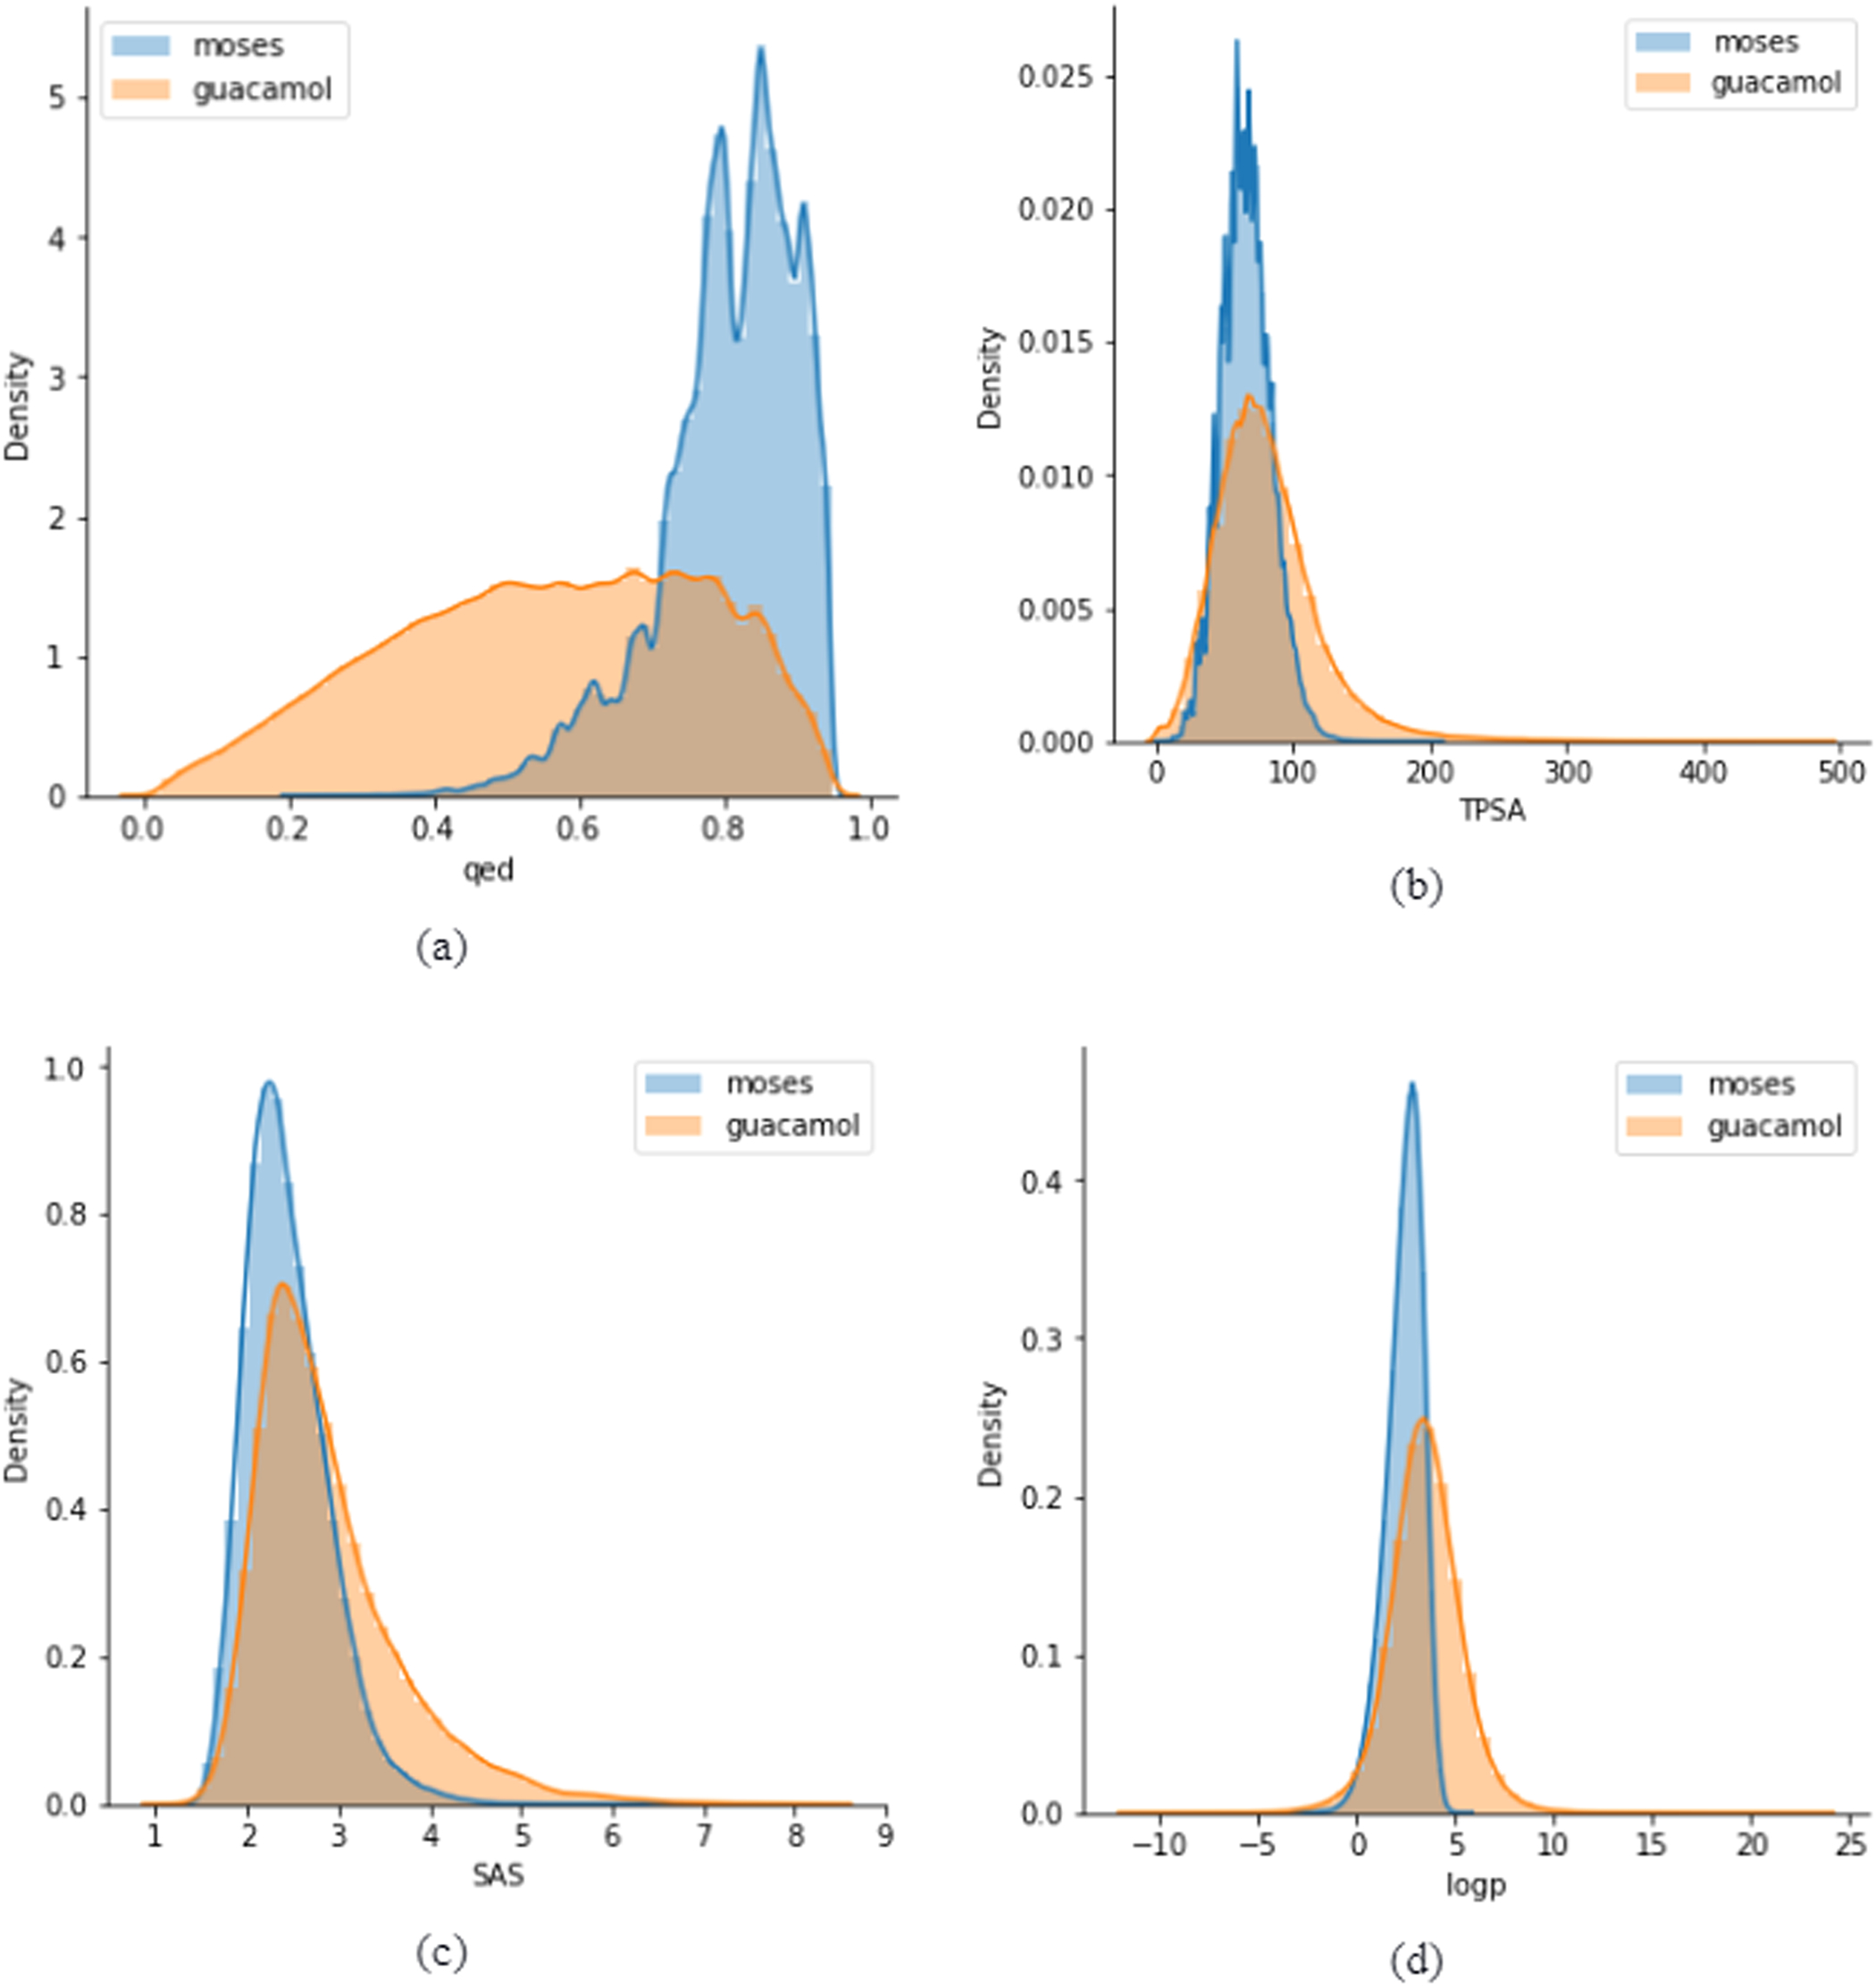
\includegraphics[width=\linewidth]{figures/2.png}
  \caption{MOSES 和 GuacaMole 中分子的性质(QED、TPSA、SAAS、aur logP)分布}
  \label{fig:2}
\end{figure}

MOSES 和 GuacaMol 数据集中药物不同属性的概率分布如图 \ref{fig:2} 所示。该分布提供了在数据集中遇到具有指定属性并落在特定范围内的药物的可能性的相对度量。 GuacaMol 数据集具有较大的属性值分布,因此用于测试模型生成具有不同属性值的分子的能力。

为了比较各种模型的性能,每个模型都被分配了预测 10,000 个分子的任务。随后,计算预测的 10,000 个分子集中有效、独特和新颖药物的百分比。

\begin{table}[H]
  \centering
  \caption{使用 MOSES 进行非条件生成训练的生成模型之间的比较}
  \label{tab:1}
  \begin{tabular}{llll}
    \hline 模型      & 有效性   & 唯一性@10 K & 新颖性   \\
    \hline AAE     & 0.937 & 0.997    & 0.793 \\
    VAE            & 0.977 & 0.998    & 0.695 \\
    CharRNN        & 0.975 & 0.999    & 0.842 \\
    LatentGAN      & 0.897 & 0.997    & 0.949 \\
    JT-VAE         & 1.0   & 0.999    & 0.914 \\
    MolGPT         & 0.994 & 1.0      & 0.797 \\
    使用相对注意力的MolGPT & 0.992 & 1.0      & 0.879 \\

    \hline
  \end{tabular}
\end{table}

表 \ref{tab:1} 给出了在 MOSES 数据集上训练的非条件生成的不同生成模型的性能比较。当使用 MOSES 训练 MolGPT 时,99.4\% 的生成化合物被识别为有效药物。当使用相对注意力而不是标准注意力时,有效性略微降低至 99.2\%。然而,所提出的具有相对注意力的模型可以比具有标准注意力的模型多预测 10\% 的新药。

\begin{figure}[H]
  \centering
  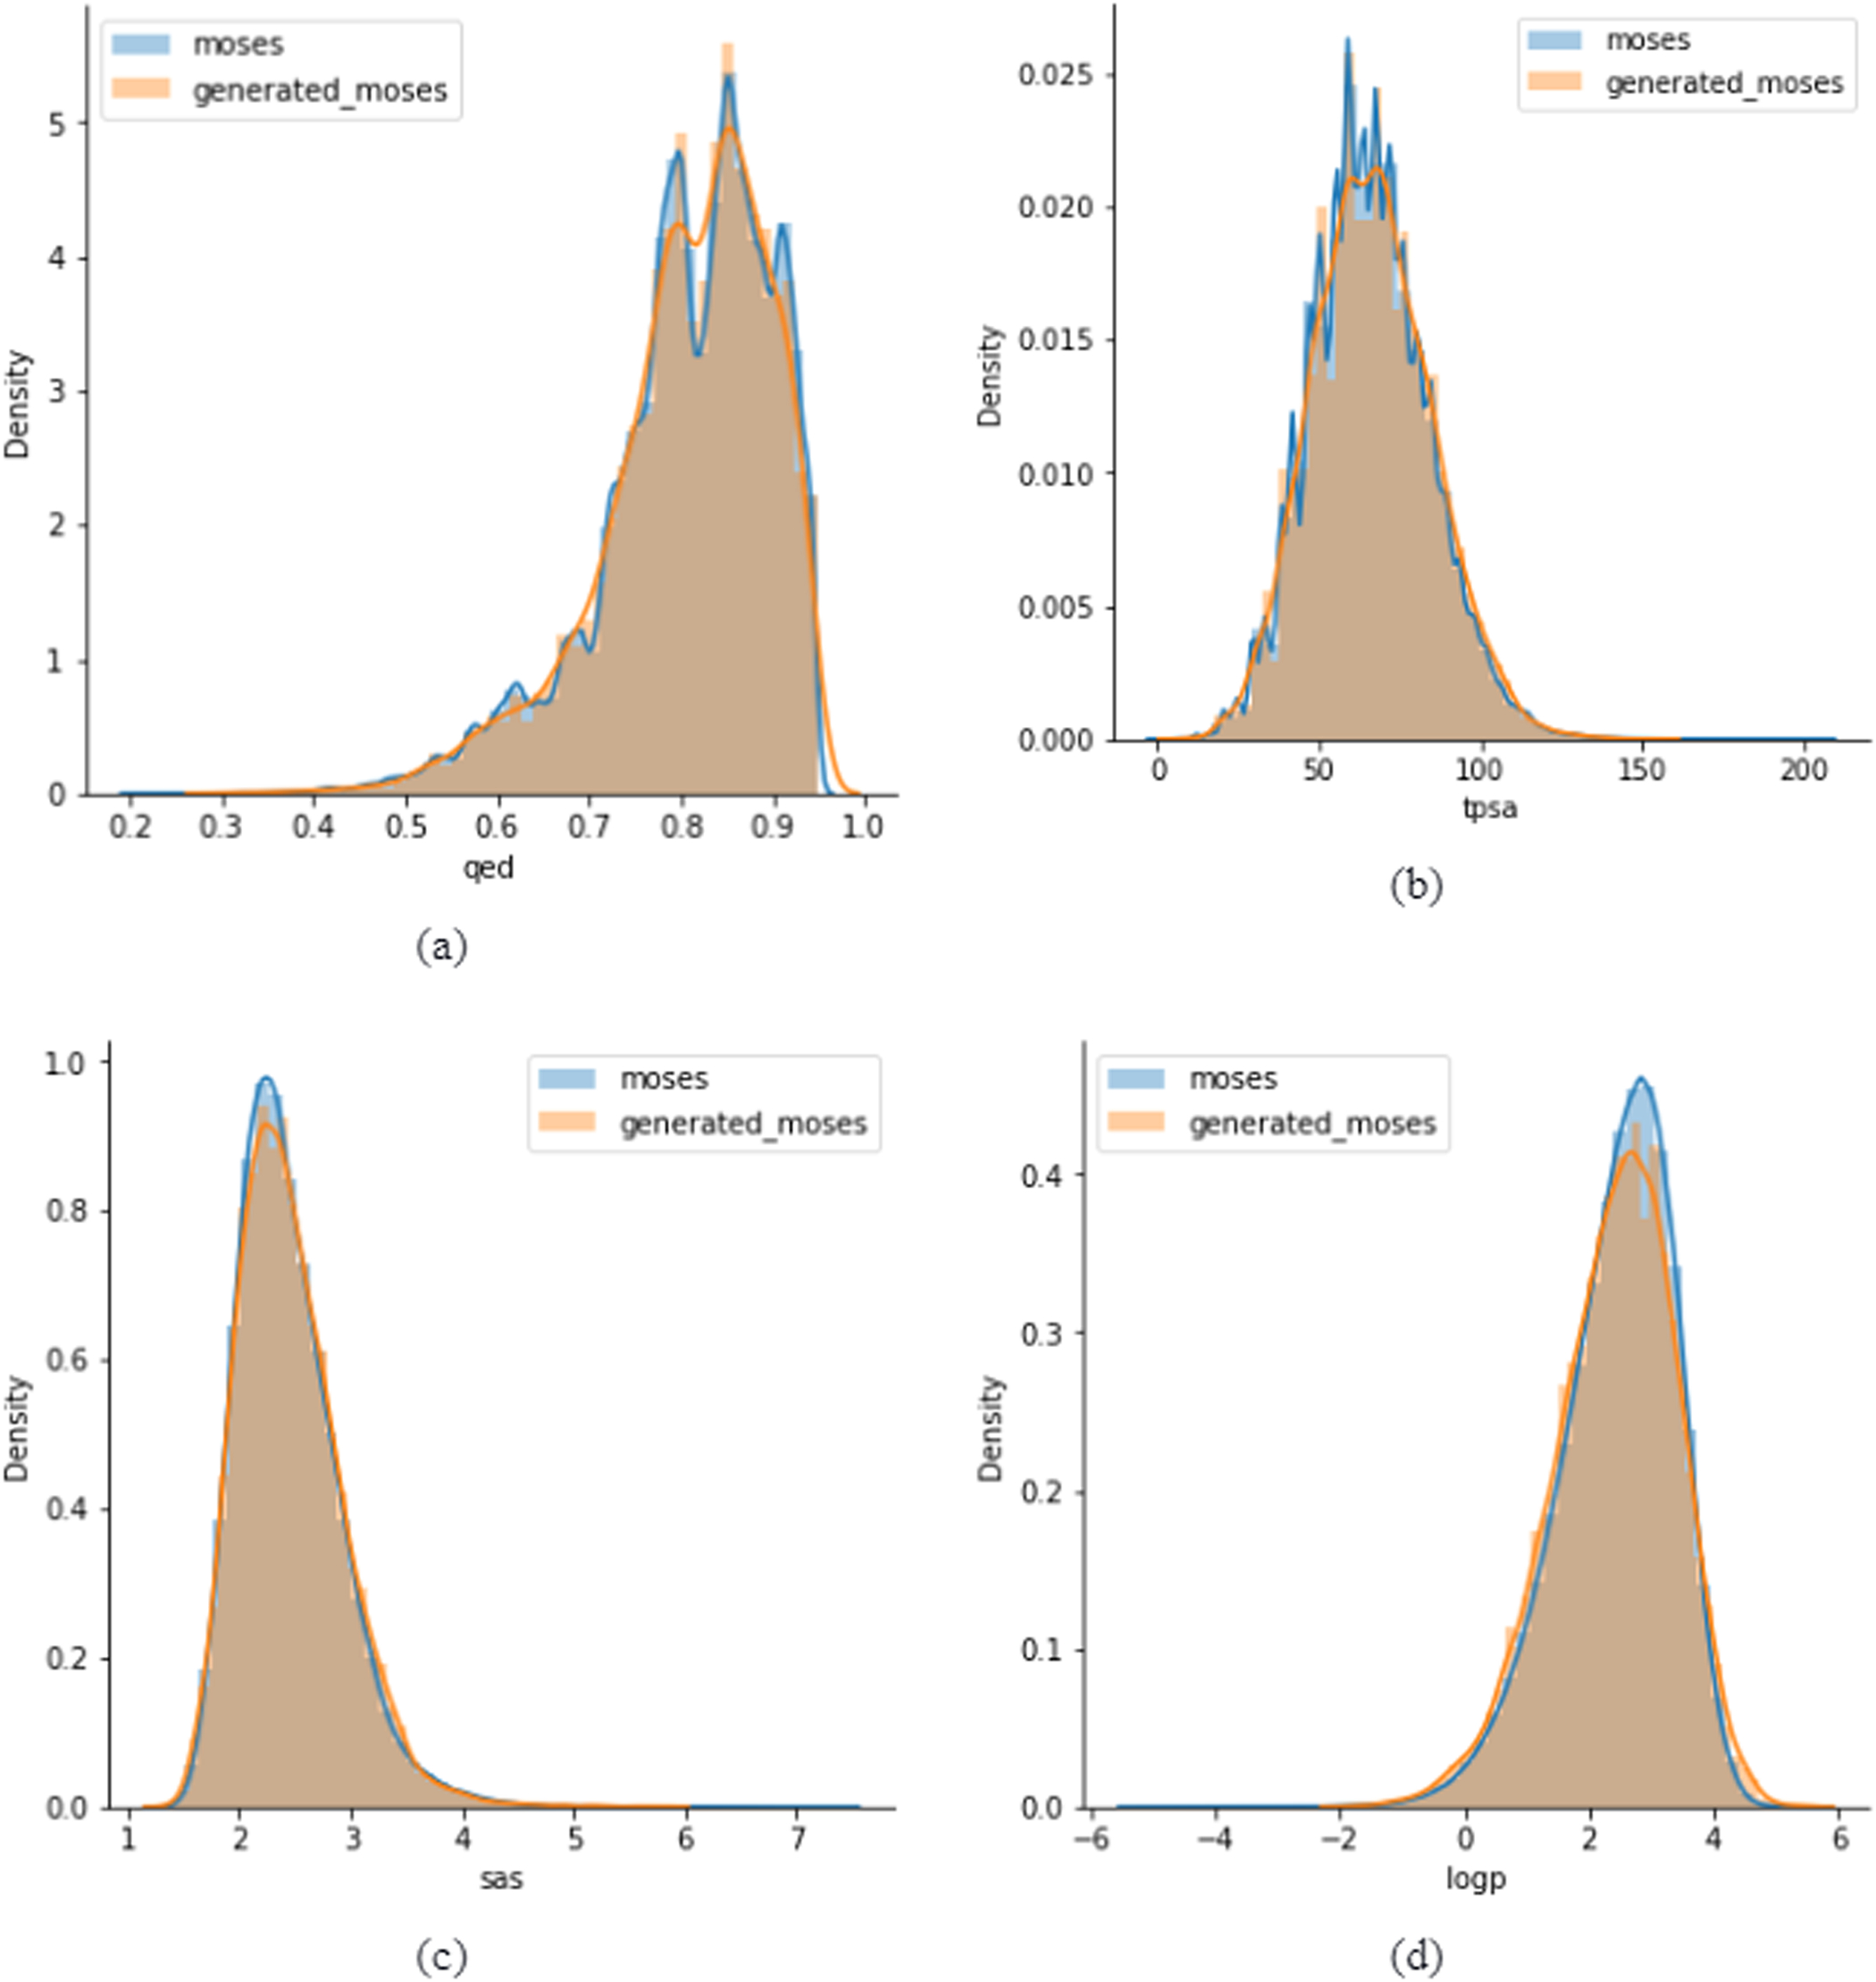
\includegraphics[width=\linewidth]{figures/3.png}
  \caption{MOSES 中分子的属性(QED、TPSA、SAS 和 logP)分布以及使用 MOSES 训练的具有相对注意力的模型生成的分子}
  \label{fig:3}
\end{figure}

图 \ref{fig:3} 说明了 MOSES 数据集与使用 MOSES 数据集训练所提出的模型后生成的药物之间的属性分布的比较。所提出的模型能够学习训练数据集的属性分布,从而生成在非条件生成期间表现出类似分布的分子。

\begin{table}[H]
  \centering
  \caption{使用 GuacaMol 进行非条件生成训练的生成模型之间的比较}
  \label{tab:2}
  \begin{tabular}{llll}
    \hline 模型       & 有效性   & 唯一性   & 新颖性   \\
    \hline VAE      & 0.870 & 0.999 & 0.974 \\
    AAE             & 0.822 & 1.0   & 0.998 \\
    ORGAN           & 0.379 & 0.841 & 0.687 \\
    SMILES LSTM     & 0.959 & 1.0   & 0.912 \\
    MolGPT          & 0.981 & 0.998 & 1.0   \\
    使用相对注意力的 MolGPT & 0.978 & 1.0   & 1.0   \\
    \hline
  \end{tabular}
\end{table}

表 \ref{tab:2} 提供了在 GuacaMol 数据集上训练的非条件生成的各种生成模型的全面比较。如表所示,具有标准注意力的 MolGPT 生成的药物的有效性达到 98.1\%,与训练集相比,所有药物都是新颖的。此外,当利用相对注意力时,该模型生成了 97.8\% 的有效药物,所有这些药物不仅新颖而且独特。

\begin{figure}[H]
  \centering
  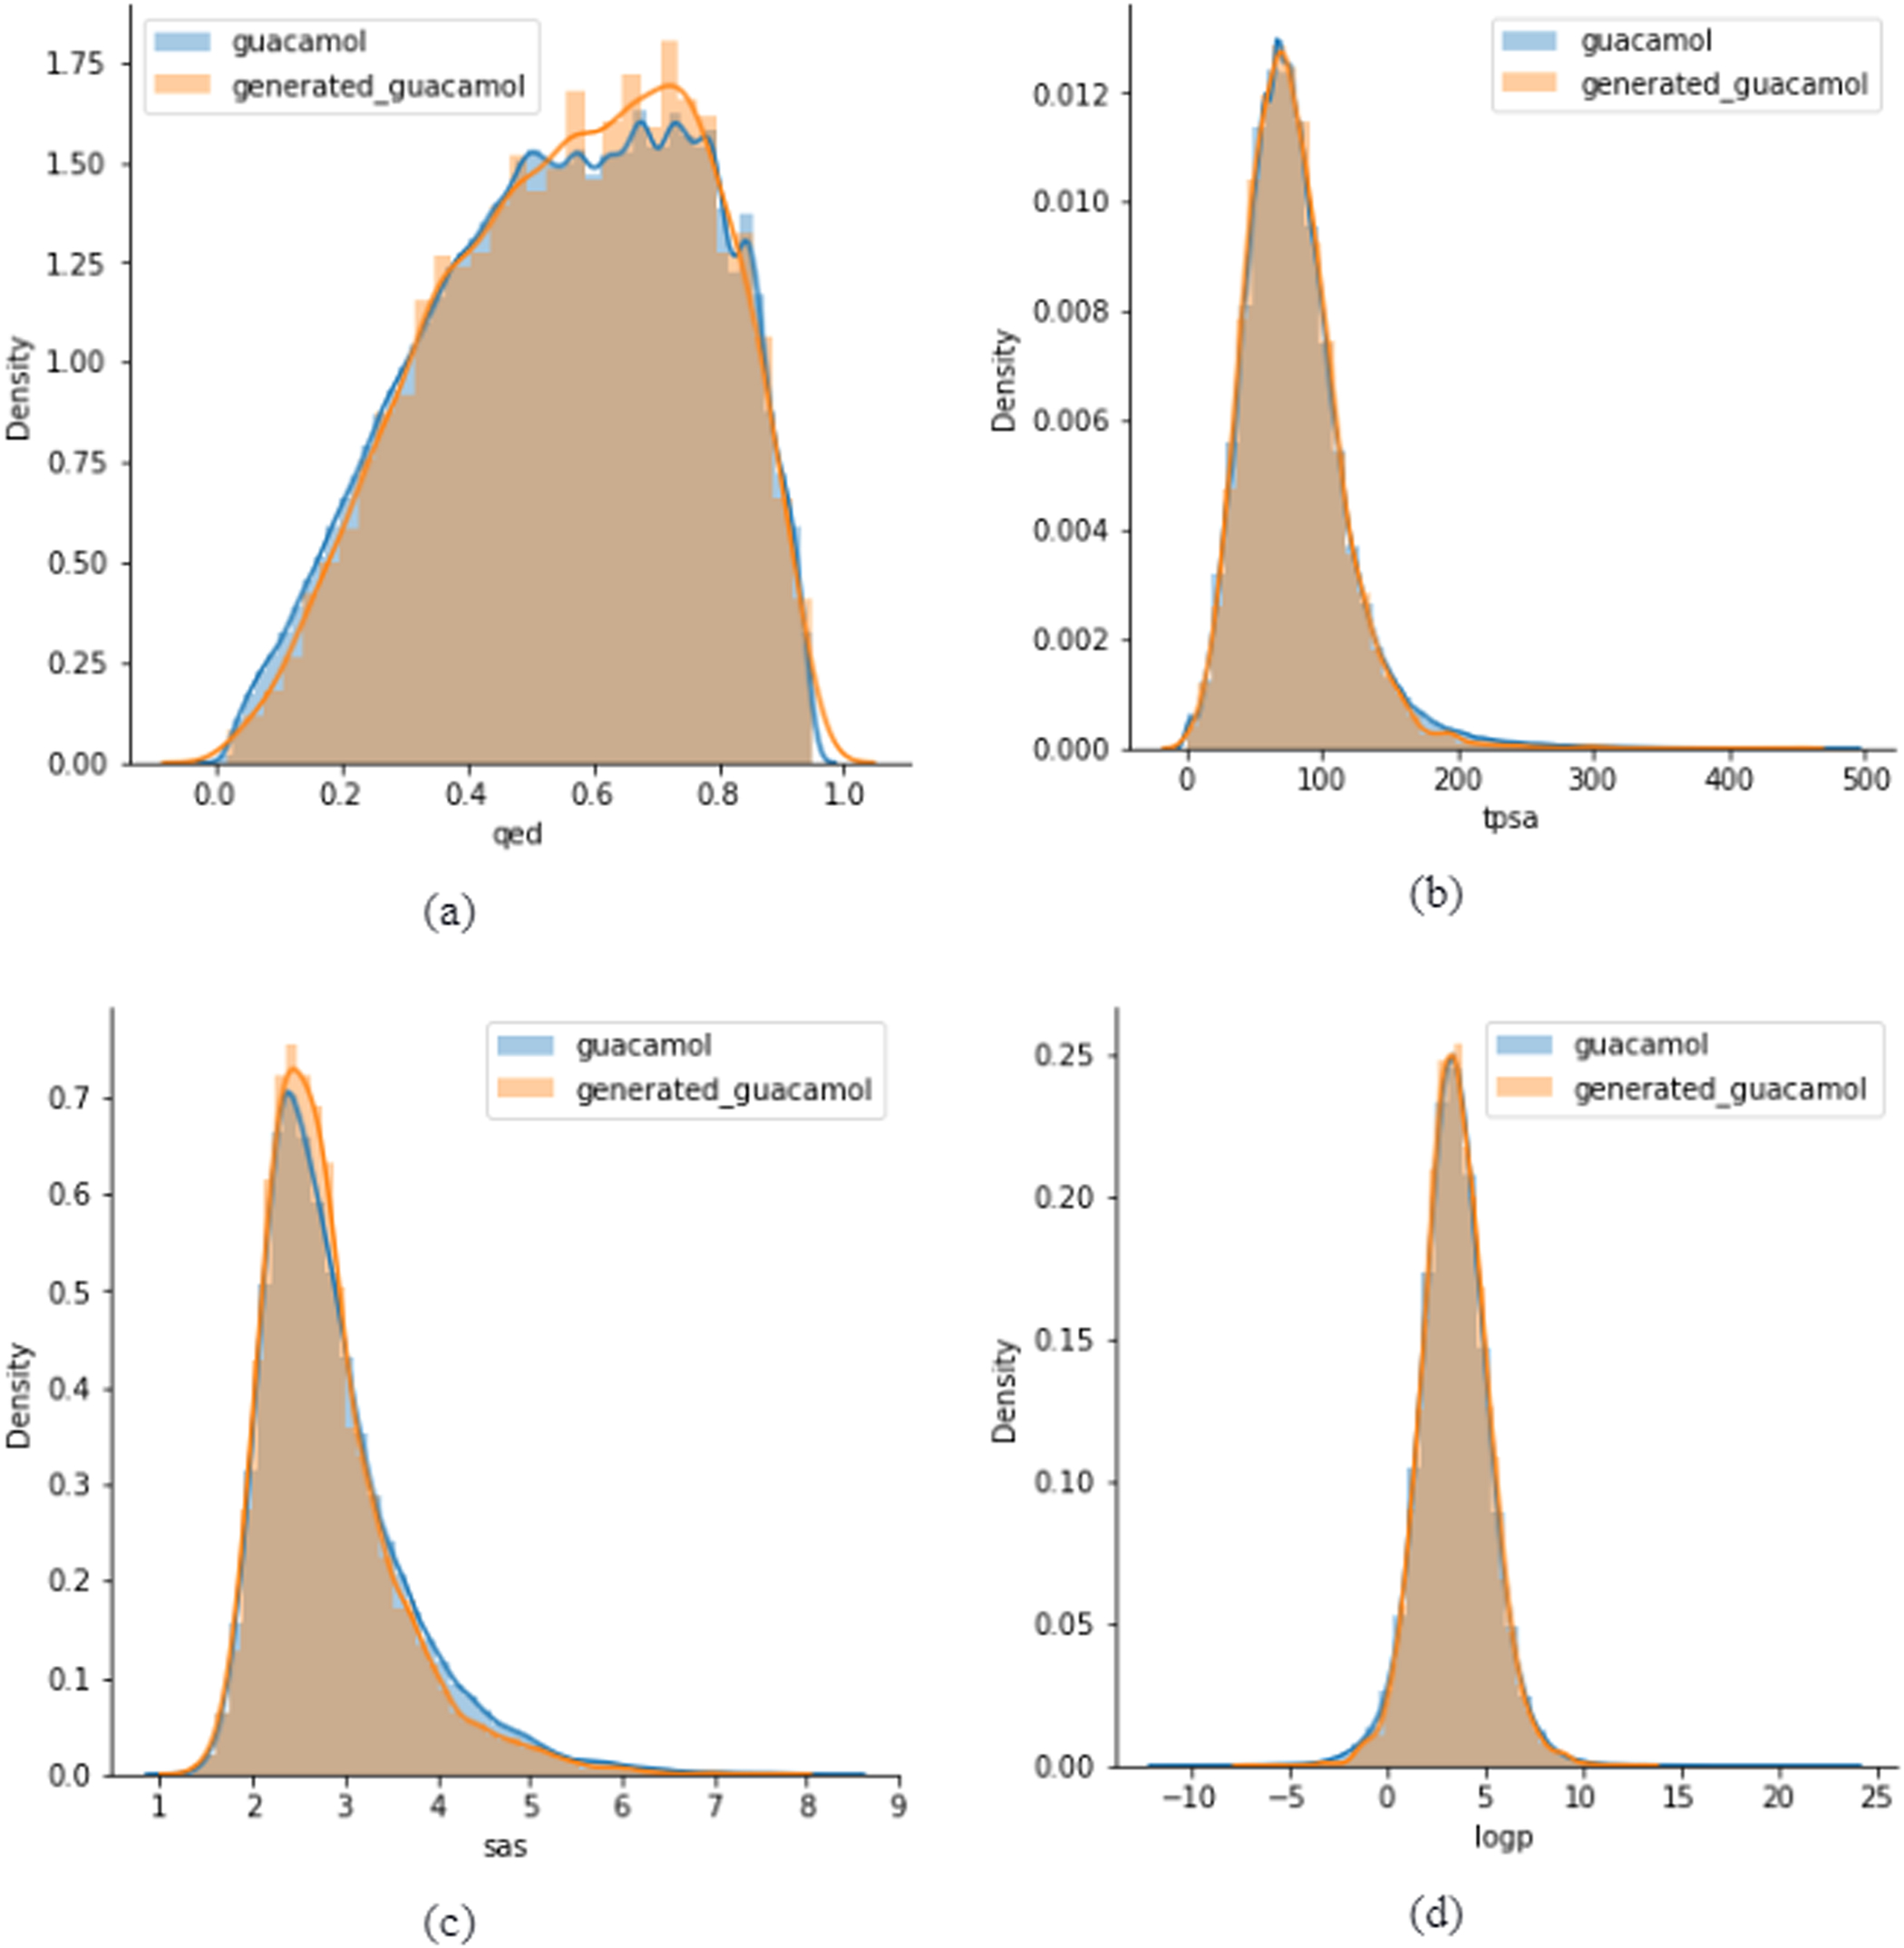
\includegraphics[width=\linewidth]{figures/4.png}
  \caption{GuacaMol 中分子的属性(QED、TPSA、SAS 和 logP)分布以及使用 GuacaMol 训练的具有相对注意力的模型生成的分子}
  \label{fig:4}
\end{figure}

图 \ref{fig:4} 比较了生成的药物和 GuacaMol 数据集的属性分布。模型预测的分子中 97.8\% 被识别为有效药物。所提出的模型证明了其从训练数据集中掌握和学习属性分布模式的能力。因此,在非条件生成过程中,模型生成的分子与训练数据集中观察到的分布非常相似。

\begin{table}[H]
  \centering
  \caption{GuacaMol 上训练标准注意力的分子条件生成的不同指标的比较}
  \label{tab:3}
  \begin{tabular}{llll}
    \hline 条件   & 有效性   & 唯一性   & 新颖性 \\
    \hline TPSA & 0.972 & 0.996 & 1.0 \\
    logP        & 0.971 & 0.998 & 1.0 \\
    SAS         & 0.977 & 0.995 & 1.0 \\
    QED         & 0.975 & 0.998 & 1.0 \\
    \hline
  \end{tabular}
\end{table}

\begin{table}[H]
  \centering
  \caption{GuacaMol 上训练的相对注意力的分子条件生成的不同指标的比较}
  \label{tab:4}
  \begin{tabular}{llll}
    \hline 条件   & 有效性   & 唯一性   & 新颖性 \\
    \hline TPSA & 0.982 & 0.999 & 1.0 \\
    log  P      & 0.969 & 1.0   & 1.0 \\
    SAS         & 0.986 & 0.997 & 1.0 \\
    QED         & 0.950 & 0.999 & 1.0 \\
    \hline
  \end{tabular}
\end{table}

当使用 GuacaMol 数据集评估具有标准注意力的 MolGPT(表 \ref{tab:3})和具有相对注意力的 MolGPT(表 \ref{tab:4})对于条件生成的性能时,在使用相对注意力的所有条件生成中观察到唯一性的适度增强。

为了评估模型在特定目标数据集上的性能,从 ExCAPEDB 中提取了两个数据集,即 HTR1A 和 S1PR1。这些数据集包含大约 72,000 个 SMILES 表达式。 MolGPT 在每个数据集上分别进行了 10 个时期的训练,同时采用了标准和相对注意机制。

\begin{table}[H]
  \centering
  \caption{S1PR1 上训练的标准注意力模型的不同指标的比较}
  \label{tab:5}
  \begin{tabular}{llll}
    \hline 条件  & 有效性   & 唯一性   & 新颖性 \\
    \hline 无条件 & 0.879 & 0.996 & 1   \\
    logP       & 0.868 & 0.994 & 1   \\
    SAS        & 0.852 & 0.997 & 1   \\
    TPSA       & 0.862 & 0.996 & 1   \\
    QED        & 0.906 & 0.976 & 1   \\
    \hline
  \end{tabular}
\end{table}


\begin{table}[H]
  \centering
  \caption{S1PR1 上训练的相对注意力模型的不同指标的比较}
  \label{tab:6}
  \begin{tabular}{llll}
    \hline 条件  & 有效性   & 唯一性   & 新颖性 \\
    \hline 无条件 & 0.87  & 0.99  & 1   \\
    logP       & 0.844 & 0.983 & 1   \\
    SAS        & 0.85  & 0.992 & 1   \\
    TPSA       & 0.855 & 0.989 & 1   \\
    QED        & 0.89  & 0.989 & 1   \\
    \hline
  \end{tabular}
\end{table}

\begin{table}[H]
  \centering
  \caption{HTR1A 上训练的标准注意力模型的不同指标的比较}
  \label{tab:7}
  \begin{tabular}{llll}
    \hline 条件  & 有效性   & 唯一性   & 新颖性 \\
    \hline 无条件 & 0.876 & 0.997 & 1   \\
    logP       & 0.801 & 0.999 & 1   \\
    SAS        & 0.849 & 0.999 & 1   \\
    TPSA       & 0.835 & 0.996 & 1   \\
    QED        & 0.878 & 0.998 & 1   \\
    \hline
  \end{tabular}
\end{table}

\begin{table}[H]
  \centering
  \caption{HTR1A 上训练的相对注意力模型的不同指标的比较}
  \label{tab:8}
  \begin{tabular}{llll}
    \hline 条件  & 有效性   & 唯一性   & 新颖性 \\
    \hline 无条件 & 0.81  & 0.991 & 1   \\
    logP       & 0.757 & 0.996 & 1   \\
    SAS        & 0.817 & 0.994 & 1   \\
    TPSA       & 0.836 & 0.99  & 1   \\
    QED        & 0.855 & 0.991 & 1   \\
    \hline
  \end{tabular}
\end{table}

\begin{figure}[H]
  \centering
  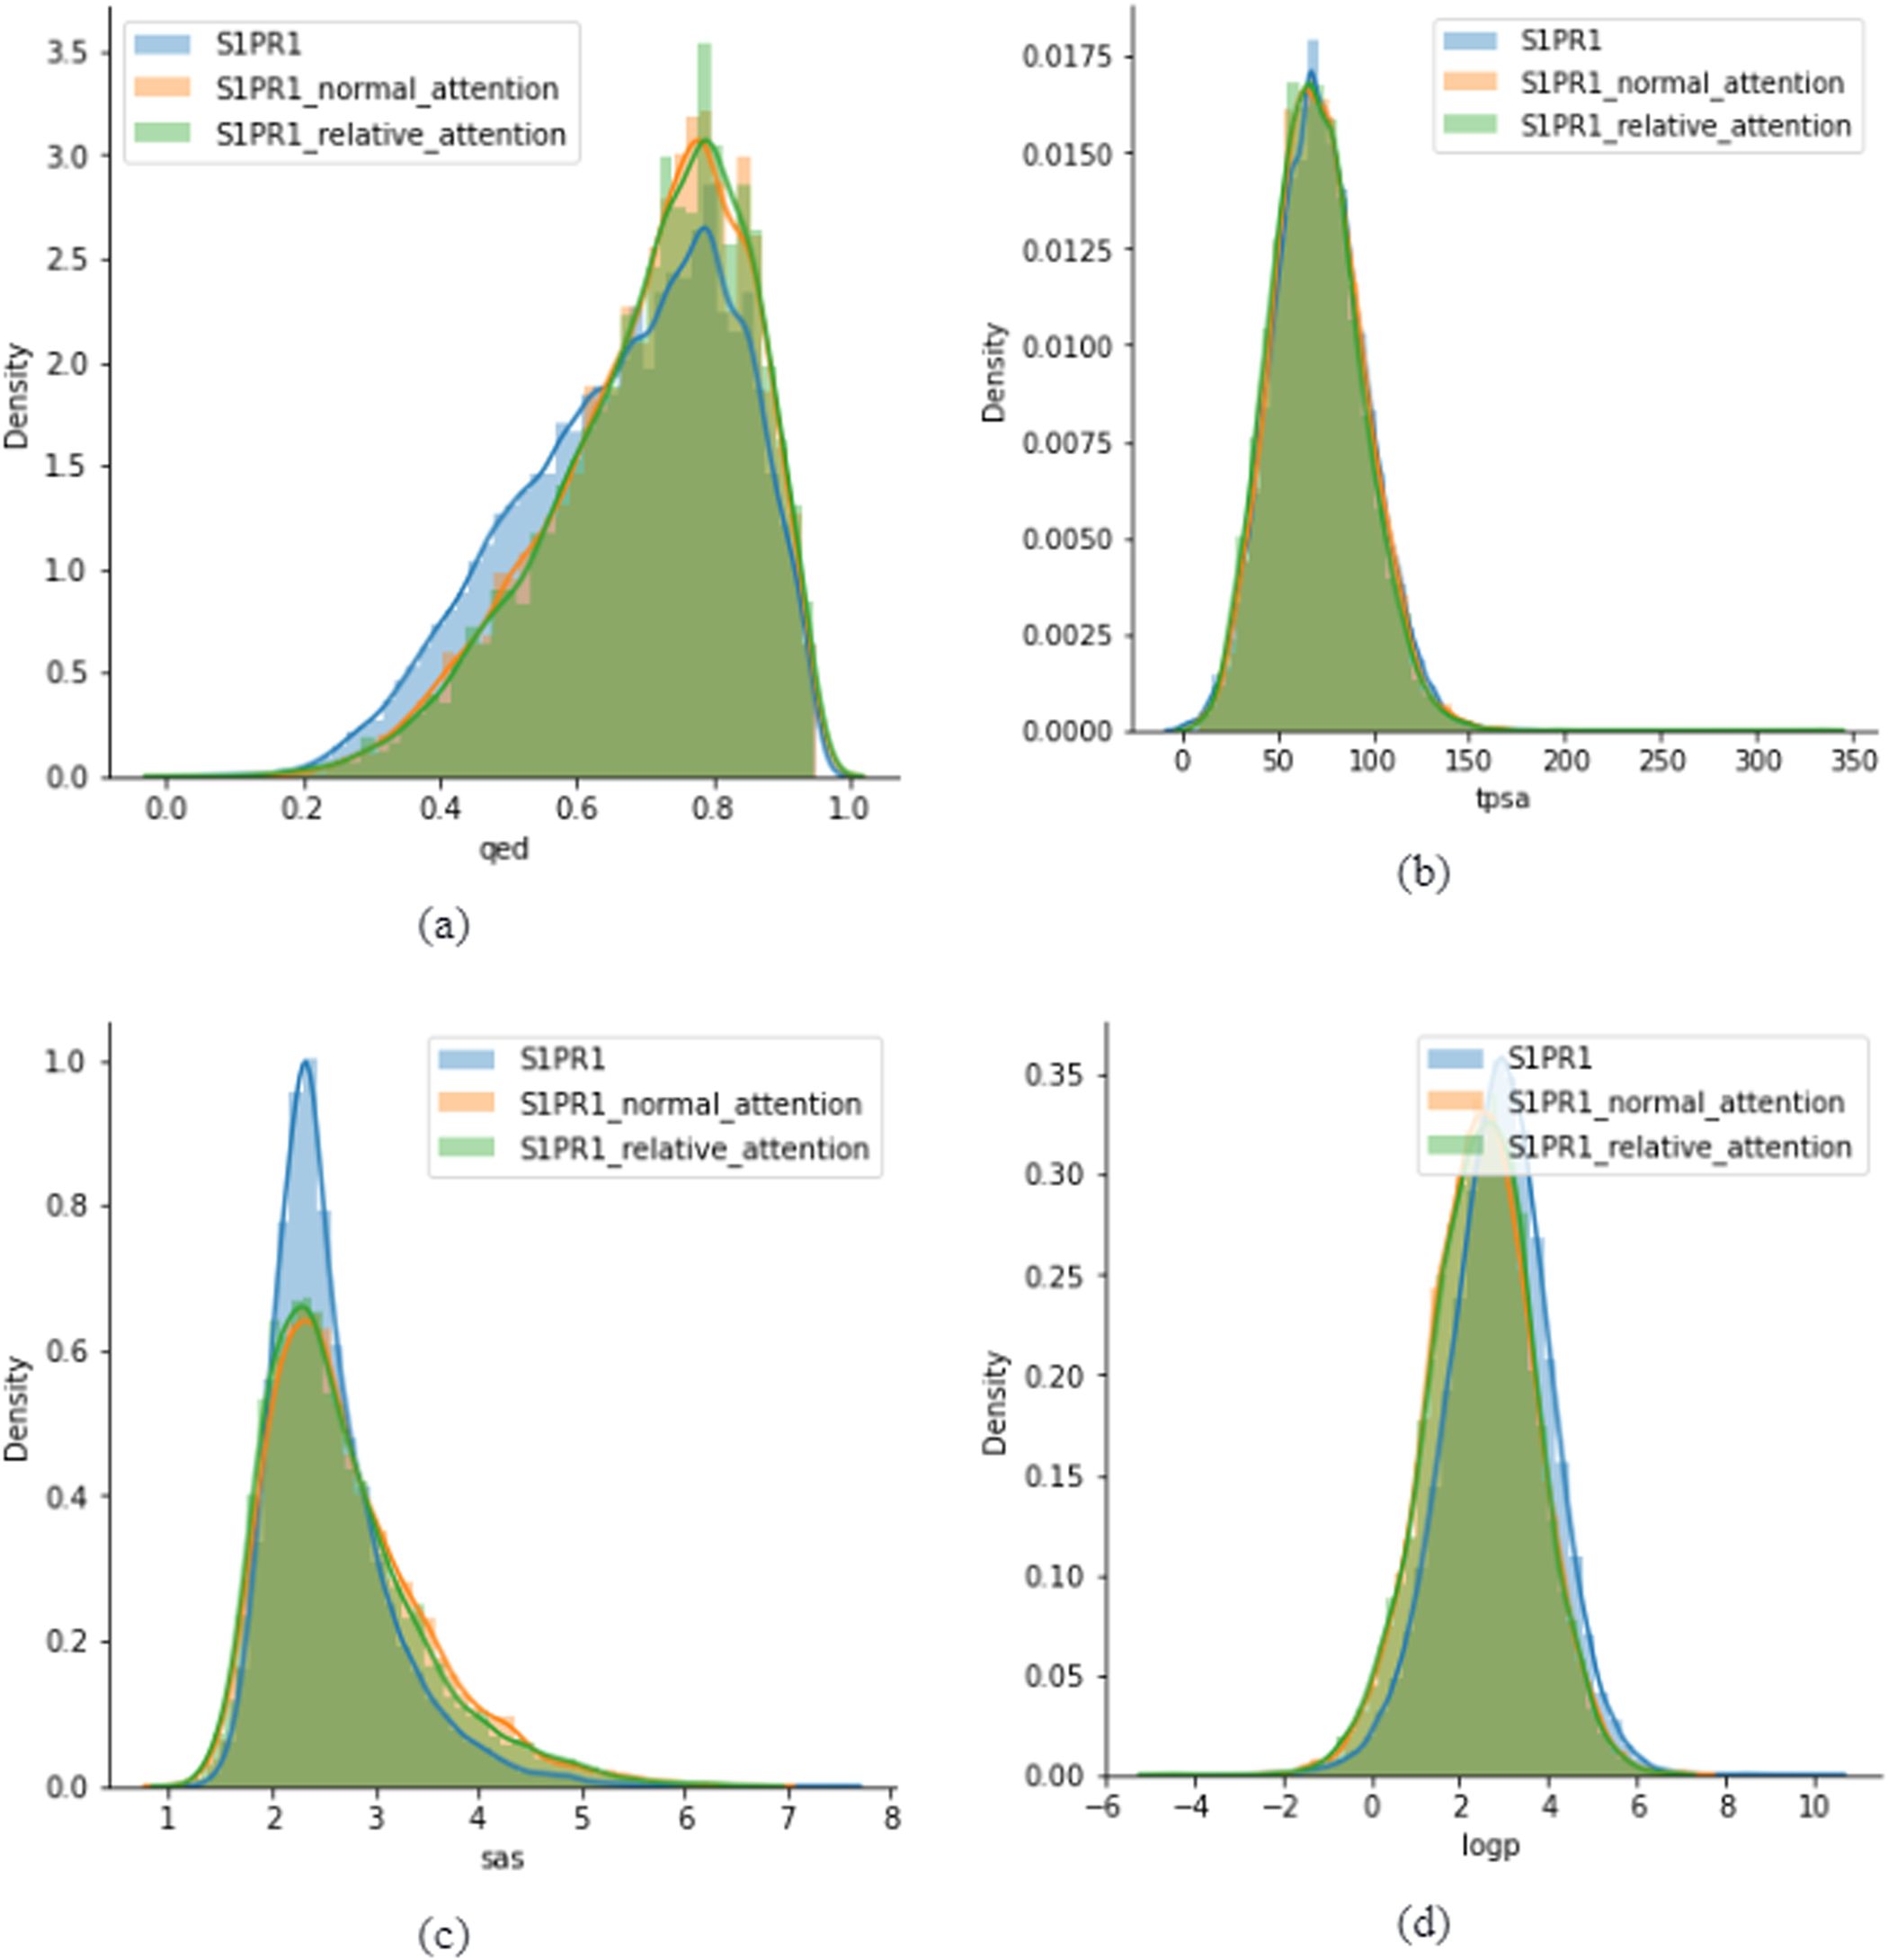
\includegraphics[width=\linewidth]{figures/5.png}
  \caption{S1PR1 中的分子以及具有标准注意力和相对注意力的模型生成的分子的属性(QED、TPSA、SAS 和 logP)分布}
  \label{fig:5}
\end{figure}

\begin{figure}[H]
  \centering
  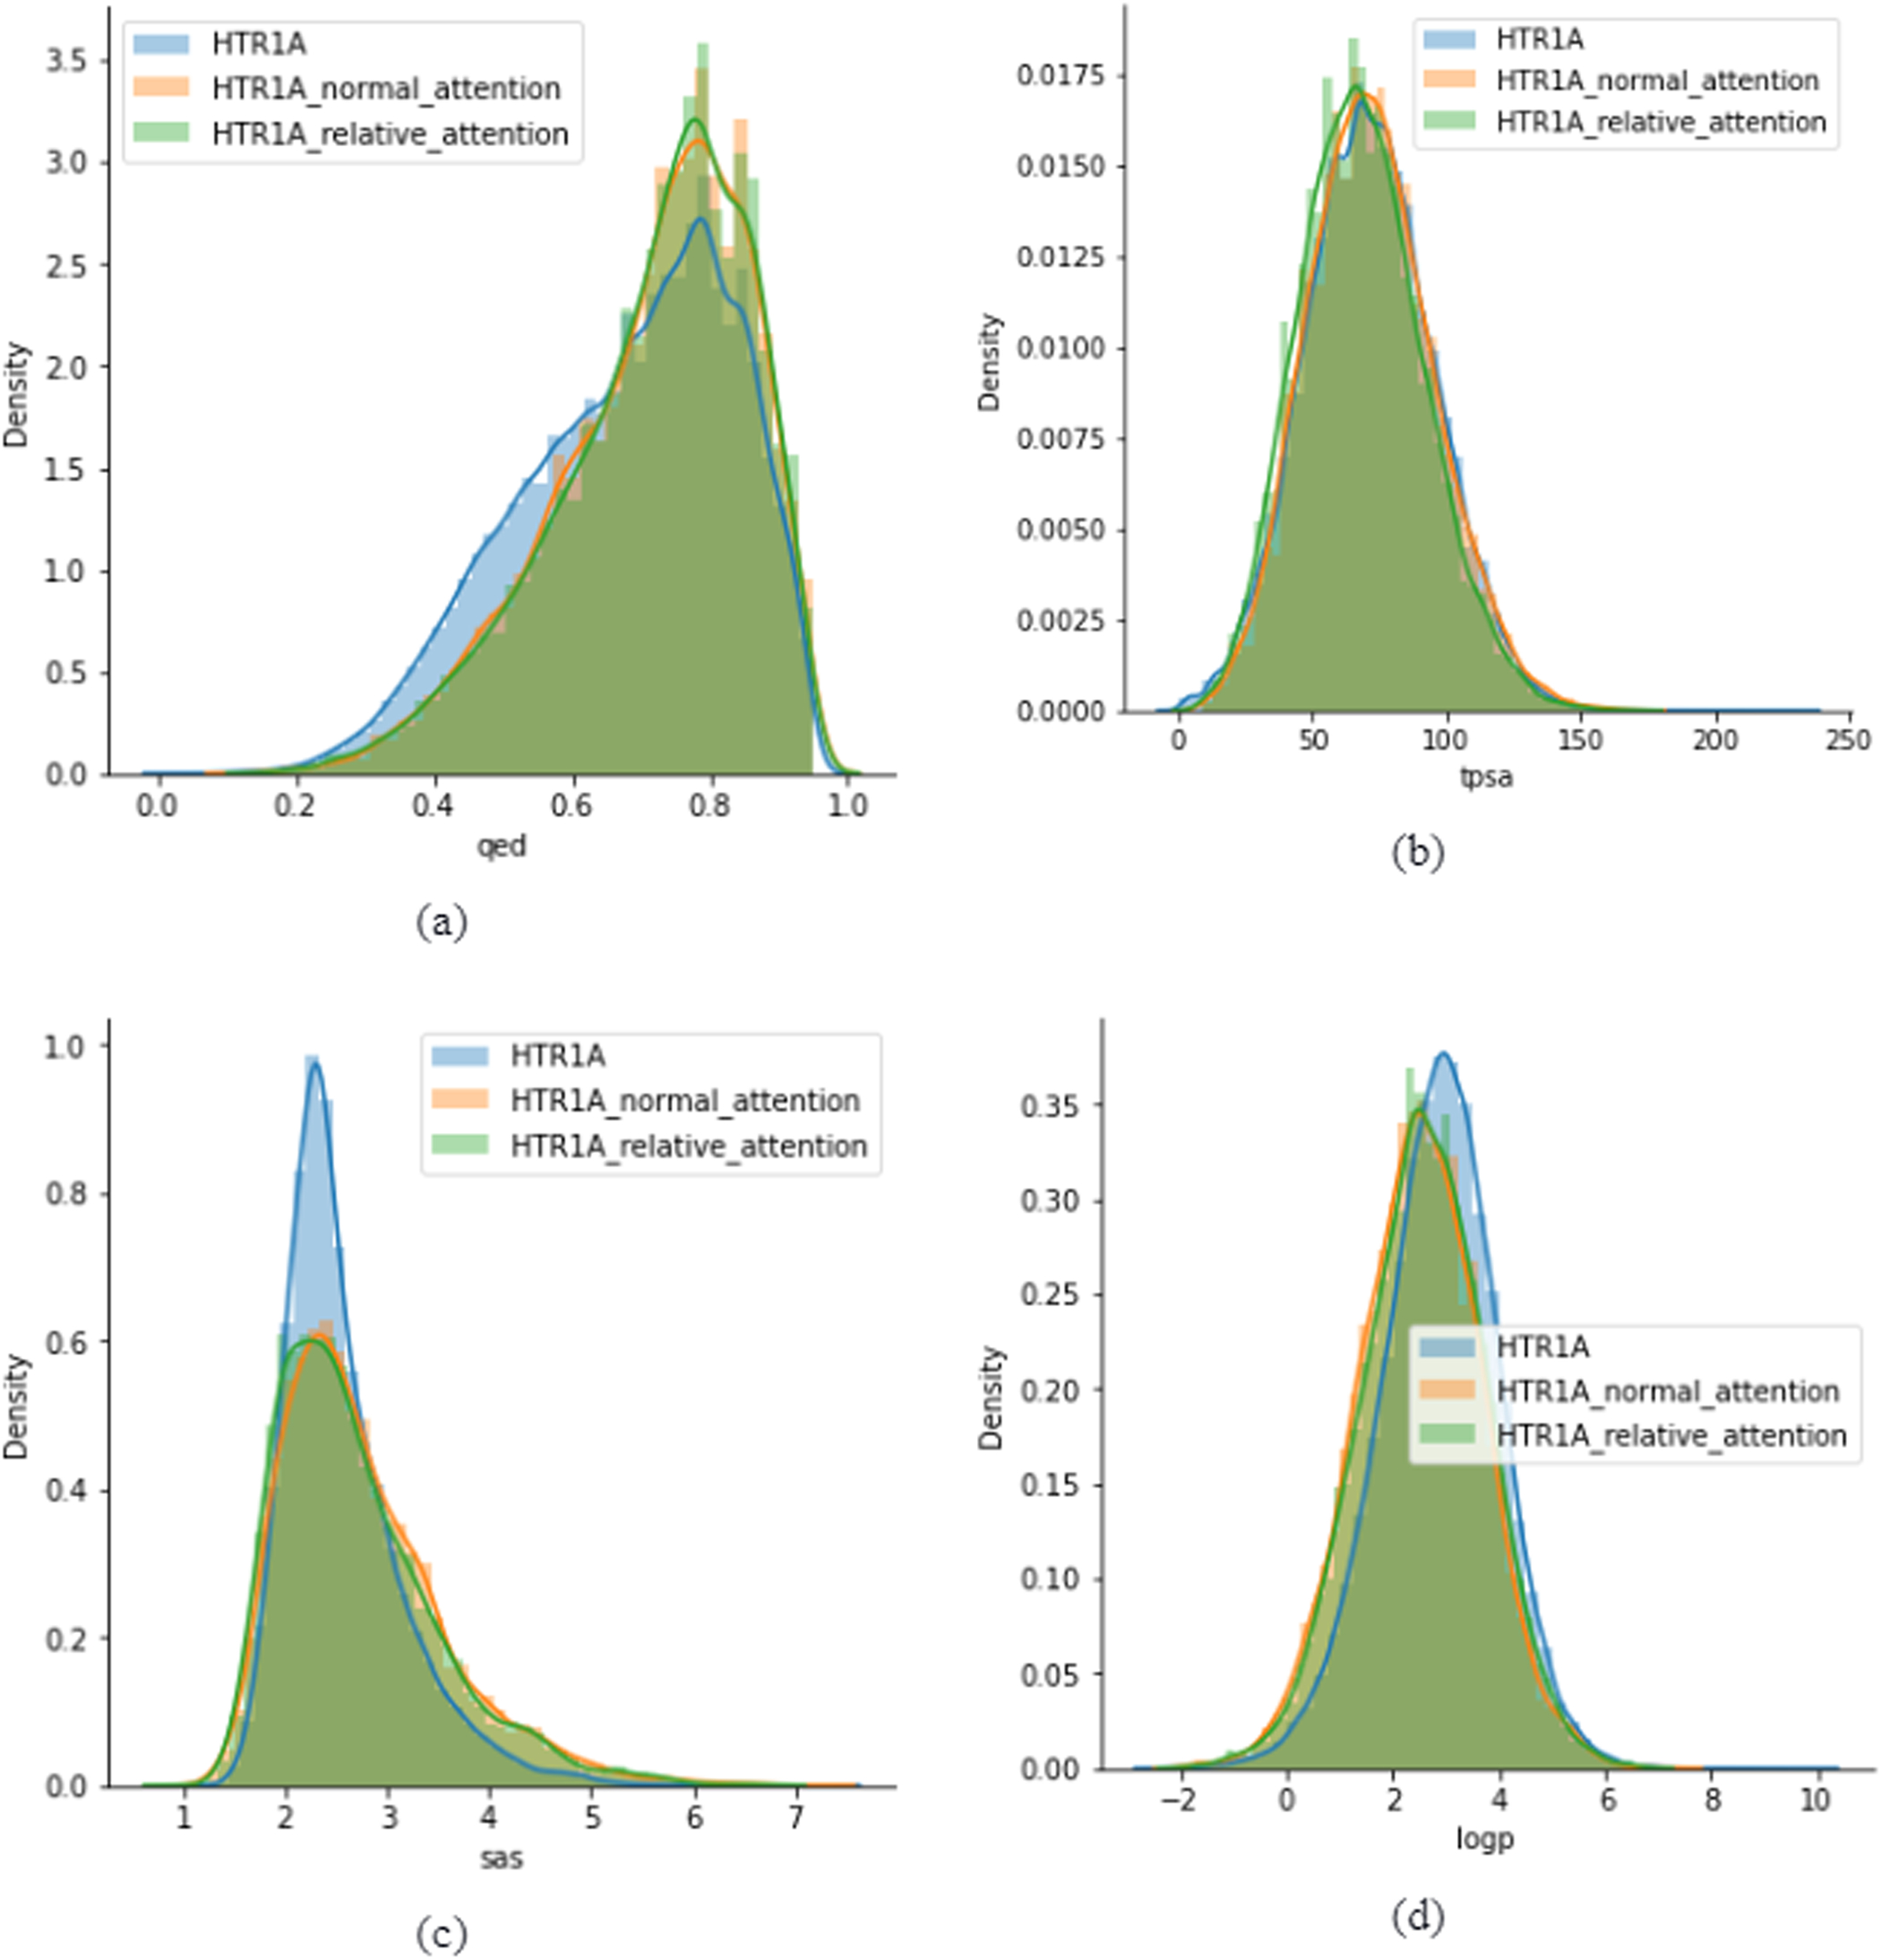
\includegraphics[width=\linewidth]{figures/6.png}
  \caption{HTR1A 数据集中分子的属性(QED、TPSA、SAS 和 logP)分布以及使用标准注意力和相对注意力训练的模型生成的分子}
  \label{fig:6}
\end{figure}

表 \ref{tab:5} 和表 \ref{tab:6} 比较了 S1PR1 数据集中标准注意力和相对注意力的表现,而表 \ref{tab:7} 和表 \ref{tab:8} 提供了 HTR1A 数据集的类似比较。图 \ref{fig:5} 和图 \ref{fig:6} 展示了S1PR1和HTR1A数据集中分子的属性分布,以及使用标准和相对注意力的模型生成的分子的属性分布。这两个模型在标准和相对关注的情况下,成功生成了具有与训练集非常相似的属性分布的分子。然而,与具有相对注意力的模型相比,具有标准注意力的 MolGPT 预测的有效分子数量略多。

HTR1A 和 S1PR1 数据集分别采样了 3400 和 800 个 SMILES,以证明相对注意力在较小数据集上的性能。后来它们被分成训练集和测试集。由于数据集大小有限,模型无法学习 SMILES 的语法。为了克服这个问题,使用了迁移学习技术。当使用迁移学习将模型的性能与较小的数据集进行比较时,通过调整相对注意力(与标准注意力相比)可以观察到显着的改进。使用 MOSES 数据集分别训练具有相对注意力的模型和具有标准注意力的模型。权重用于训练特定于目标的较小数据集。由于训练数据集较小,该模型配置为仅预测 1000 个分子。

\begin{table}[H]
  \centering
  \caption{使用迁移学习对采样 S1PR1 非条件生成训练的标准注意力模型和相对注意力模型的比较}
  \label{tab:9}
  \begin{tabular}{llll}
    \hline 模型       & 有效性   & 唯一性   & 新颖性   \\
    \hline ModelGPT & 0.47  & 0.94  & 0.996 \\
    使用相对注意力的 MolGPT & 0.588 & 0.958 & 0.979 \\
    \hline
  \end{tabular}
\end{table}

表 \ref{tab:9} 提供了使用标准注意力和使用采样的 S1PR1 数据集和迁移学习进行非条件生成的相对注意力进行训练的性能比较。当进行标准注意力训练时,只有 47\% 的预测分子被识别为有效药物。然而,当进行相对关注的训练时,该有效性百分比增加到 58.8\%,从而显着提高 11.8\%。

\begin{table}[H]
  \centering
  \caption{使用迁移学习在采样 S1PR1 上训练条件生成的相对注意力模型的不同指标的比较}
  \label{tab:10}
  \begin{tabular}{llll}
    \hline 条件 & 有效性   & 唯一性   & 新颖性   \\
    logP      & 0.724 & 0.86  & 0.984 \\
    TPSA      & 0.739 & 0.794 & 0.988 \\
    SAS       & 0.708 & 0.99  & 0.99  \\
    QED       & 0.685 & 0.991 & 0.99  \\
    \hline
  \end{tabular}
\end{table}


\begin{figure}[H]
  \centering
  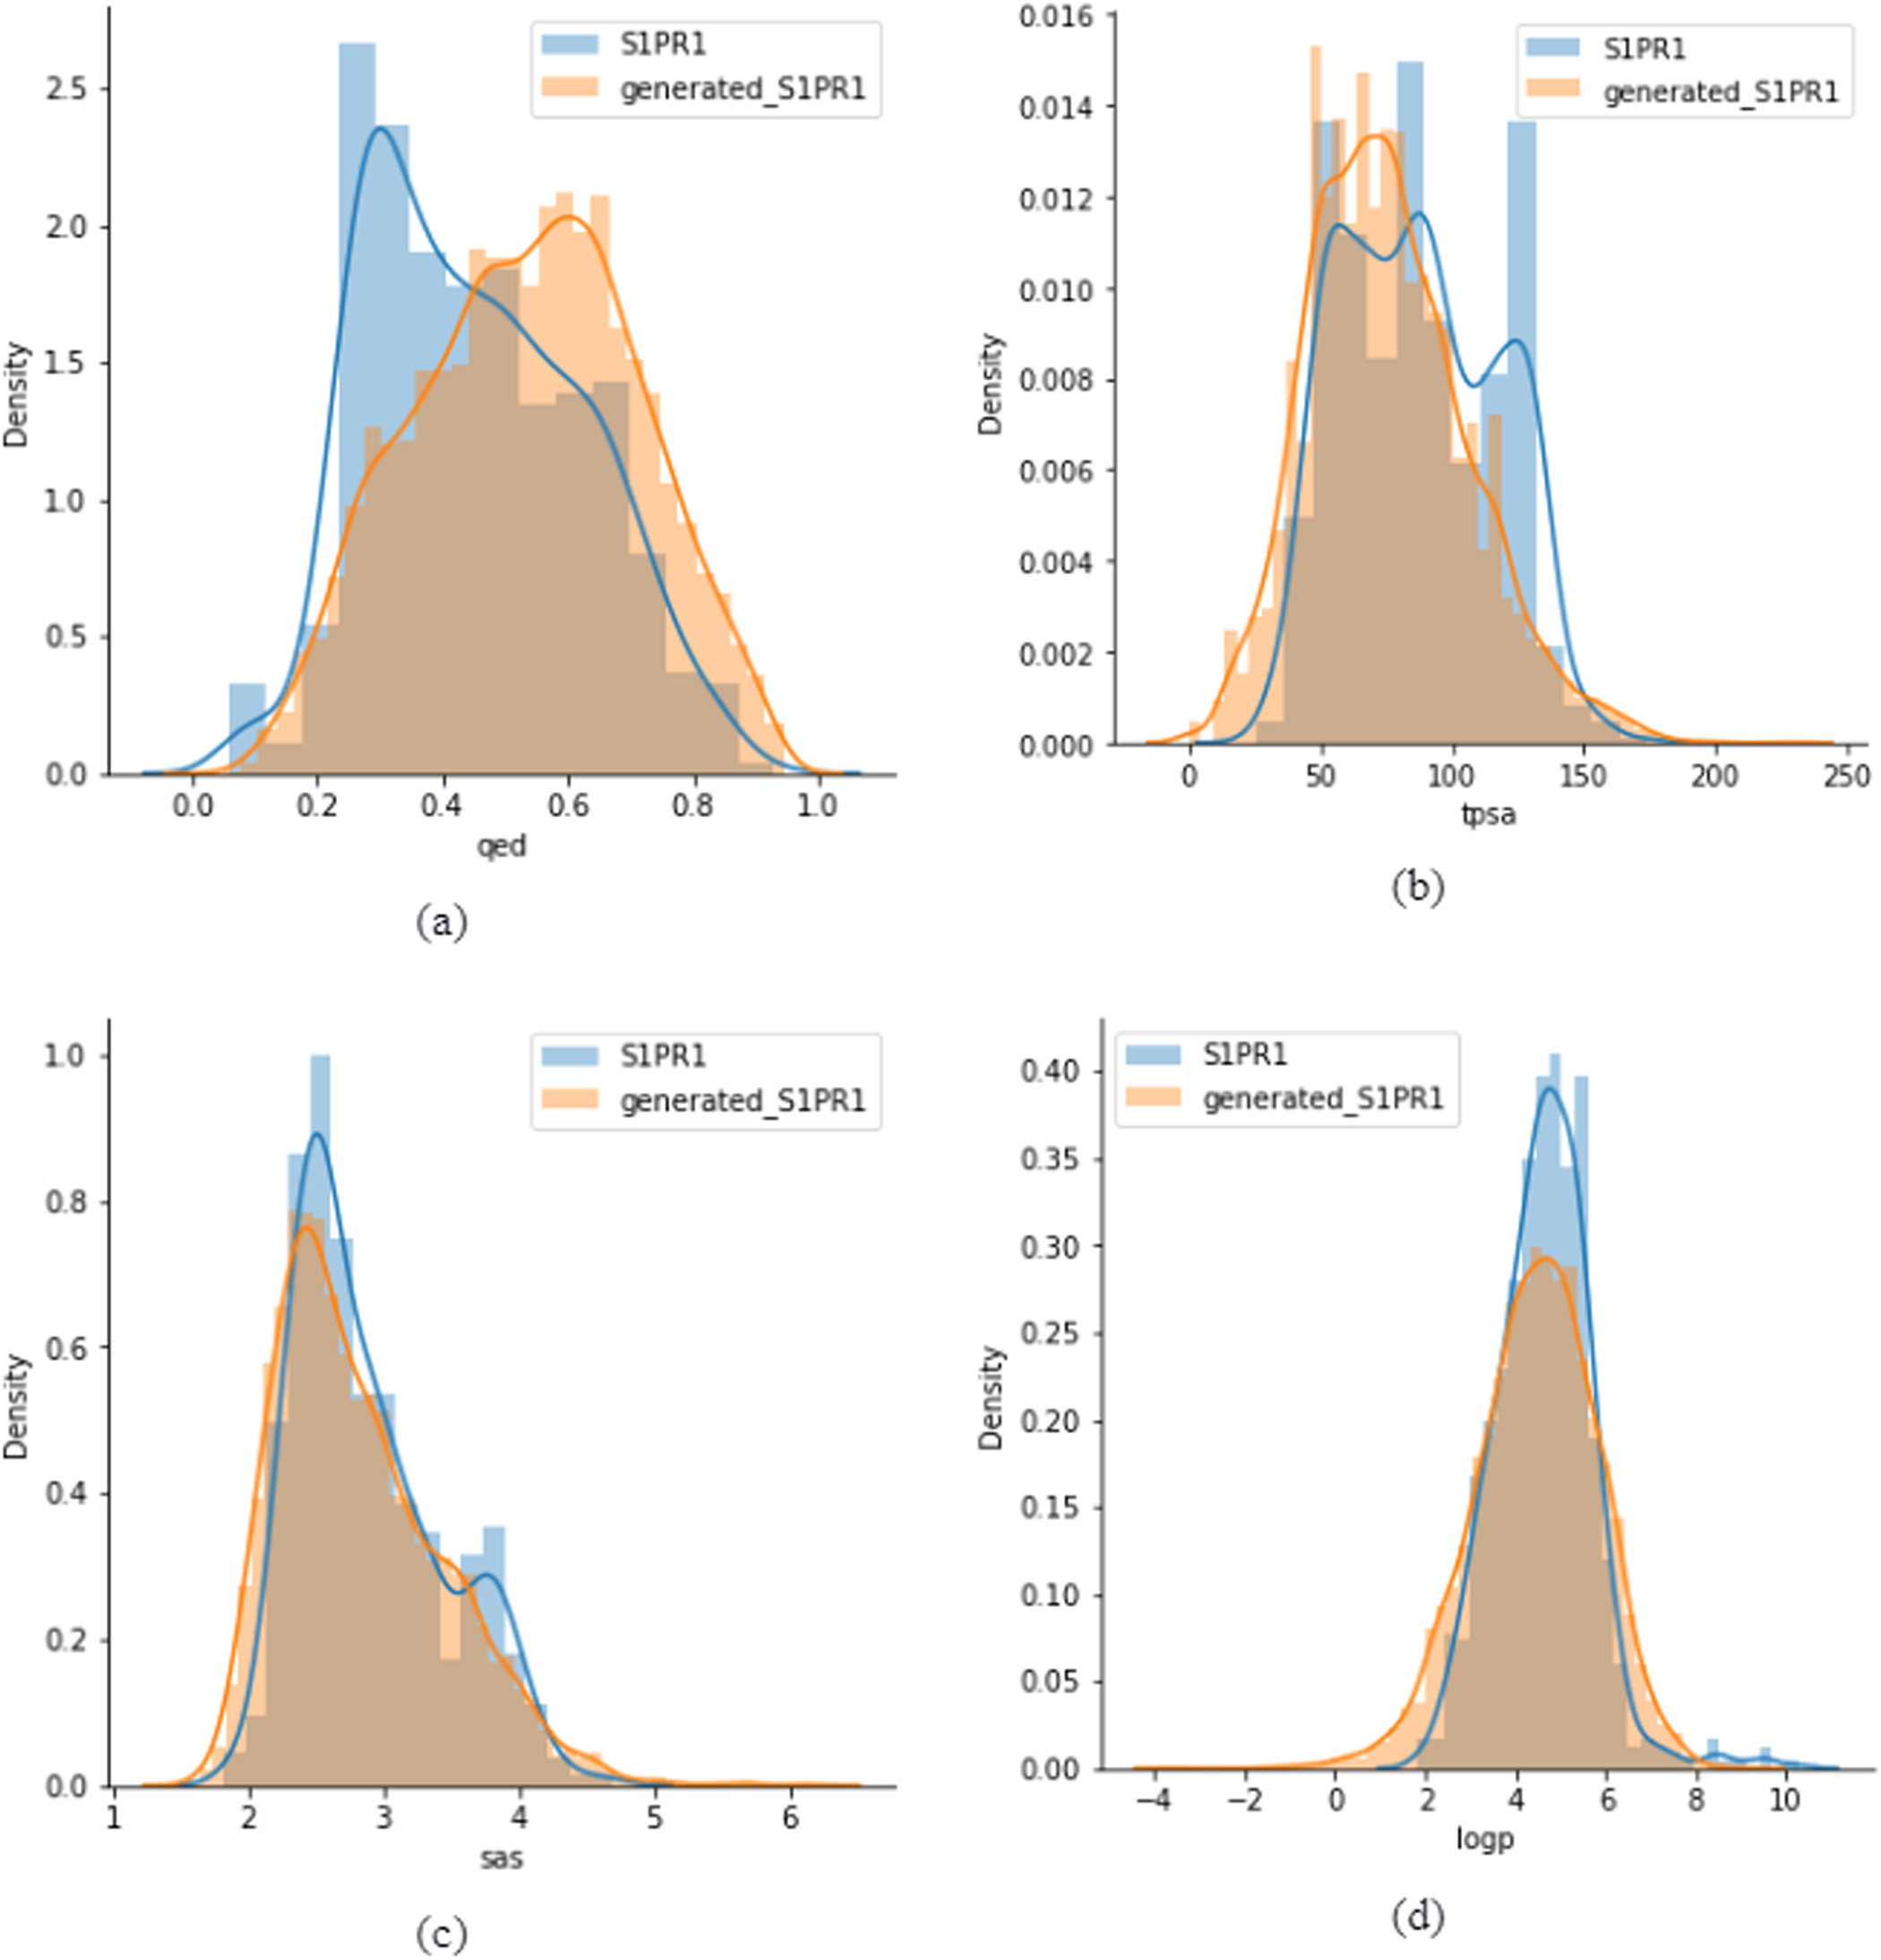
\includegraphics[width=\linewidth]{figures/7.png}
  \caption{采样的 S1PR1 中的分子和相对关注生成的分子的属性(QED、TPSA、SAS 和 logP)分布}
  \label{fig:7}
\end{figure}

在表 \ref{tab:10} 中,报告了使用采样的 S1PR1 数据集进行条件生成的具有相对关注的模型的性能。此外,图 \ref{fig:7} 直观地展示了采样的 S1PR1 数据集中分子的属性分布以及使用相对注意力生成的分子。

\begin{table}[H]
  \centering
  \caption{使用迁移学习使用采样 HTR1A 非条件生成训练的标准和相对注意力模型之间的比较}
  \label{tab:11}
  \begin{tabular}{llll}
    \hline 模型       & 有效性   & 唯一性   & 新颖性   \\
    \hline ModelGPT & 0.852 & 0.928 & 0.859 \\
    使用相对注意力的 MolGPT & 0.863 & 0.945 & 0.877 \\
    \hline
  \end{tabular}
\end{table}

表 \ref{tab:11} 展示了使用采样的 HTR1A 数据集和迁移学习进行非条件生成的标准注意力和相对注意力训练的模型之间的性能比较。采样数据集包含 3400 个 SMILES。具有标准注意力的 MolGPT 预测了 85.2\% 的有效药物。然而,当采用相对关注时,有效性增加到 86.3\%。

\begin{table}[H]
  \centering
  \caption{使用迁移学习使用采样 HTR1A 非条件生成训练的标准和相对注意力模型之间的比较}
  \label{tab:12}
  \begin{tabular}{llll}
    \hline 条件 & 有效性   & 唯一性   & 新颖性   \\
    logP      & 0.804 & 0.824 & 0.947 \\
    TPSA      & 0.878 & 0.706 & 0.946 \\
    SAS       & 0.861 & 0.684 & 0.934 \\
    QED       & 0.893 & 0.793 & 0.946 \\
    \hline
  \end{tabular}
\end{table}

\begin{figure}[H]
  \centering
  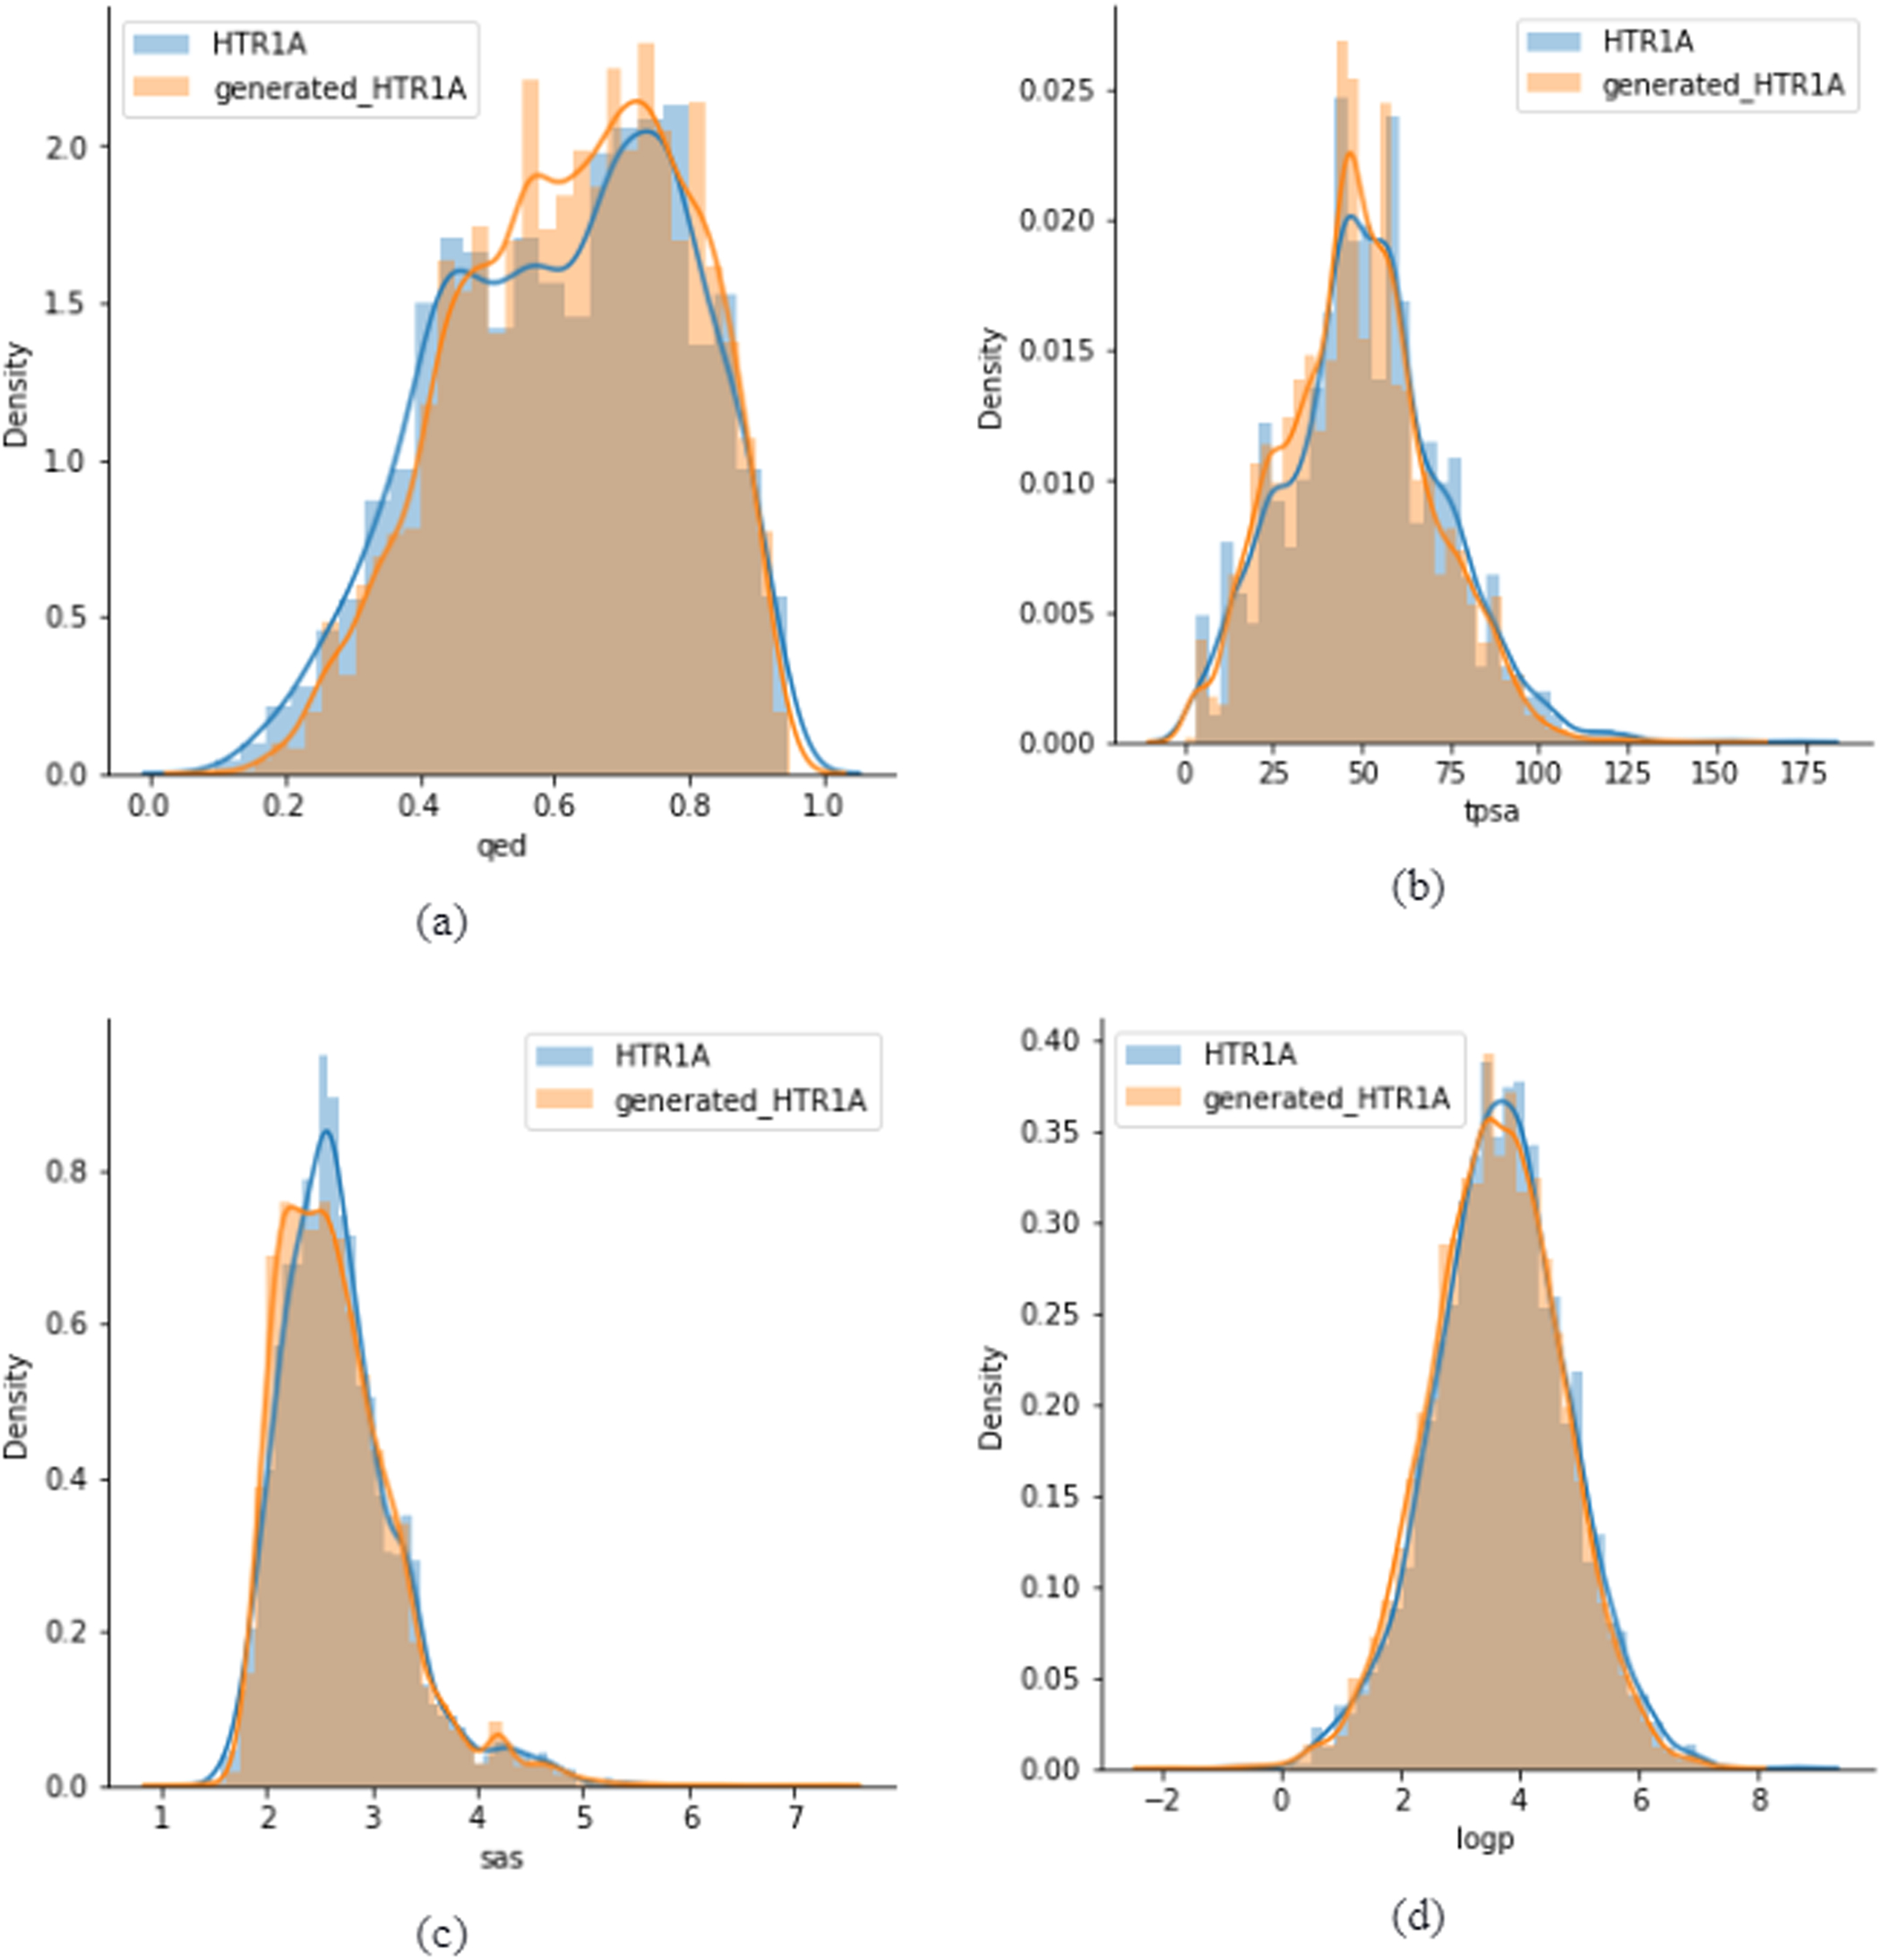
\includegraphics[width=\linewidth]{figures/8.png}
  \caption{采样的 HTR1A 中分子的特性(QED、TPSA、SAS 和 logP)分布以及相对关注生成的分子}
  \label{fig:8}
\end{figure}

表 \ref{tab:12} 报告了使用采样的 HTR1A 数据集相对关注条件生成的模型的性能。此外,图 \ref{fig:8} 可视化了采样的 HTR1A 数据集中分子的属性分布,以及使用相对注意力生成的分子。


图 \ref{fig:7} 和图 \ref{fig:8} 显示,即使数据集大小有限,具有相对注意力的模型也能够生成具有与训练集相似的属性分布的分子。

\begin{table}[H]
  \centering
  \caption{使用转移学习对 EGFR 非条件生成进行标准注意力和相对注意力训练的模型之间的比较}
  \label{tab:13}
  \begin{tabular}{llll}
    \hline 模型       & 有效性   & 唯一性   & 新颖性   \\
    \hline ModelGPT & 0.586 & 0.978 & 0.998 \\
    使用相对注意力的 MolGPT & 0.713 & 0.959 & 0.989 \\
    \hline
  \end{tabular}
\end{table}

表 \ref{tab:13} 提供了使用 EGFR 数据集进行非条件生成的标准注意力和相对注意力训练模型的性能比较。标准注意力模型生成了 58.6\% 的有效药物,而相对注意力模型在生成的 1000 个分子中获得了 71.3\% 的较高有效率。这表明有效性显着提高了 12.6\%。

\begin{table}[H]
  \centering
  \caption{使用转移学习对 EGFR 进行条件生成训练的模型的不同指标的比较}
  \label{tab:14}
  \begin{tabular}{llll}
    \hline 条件 & 有效性   & 唯一性   & 新颖性   \\
    logP      & 0.655 & 0.912 & 0.994 \\
    TPSA      & 0.757 & 0.841 & 0.993 \\
    SAS       & 0.717 & 0.854 & 0.985 \\
    QED       & 0.757 & 0.885 & 0.993 \\
    \hline
  \end{tabular}
\end{table}

表 \ref{tab:14} 显示了在 EGFR 数据集上训练相对注意力模型的性能,以使用迁移学习进行条件生成。

\begin{figure}[H]
  \centering
  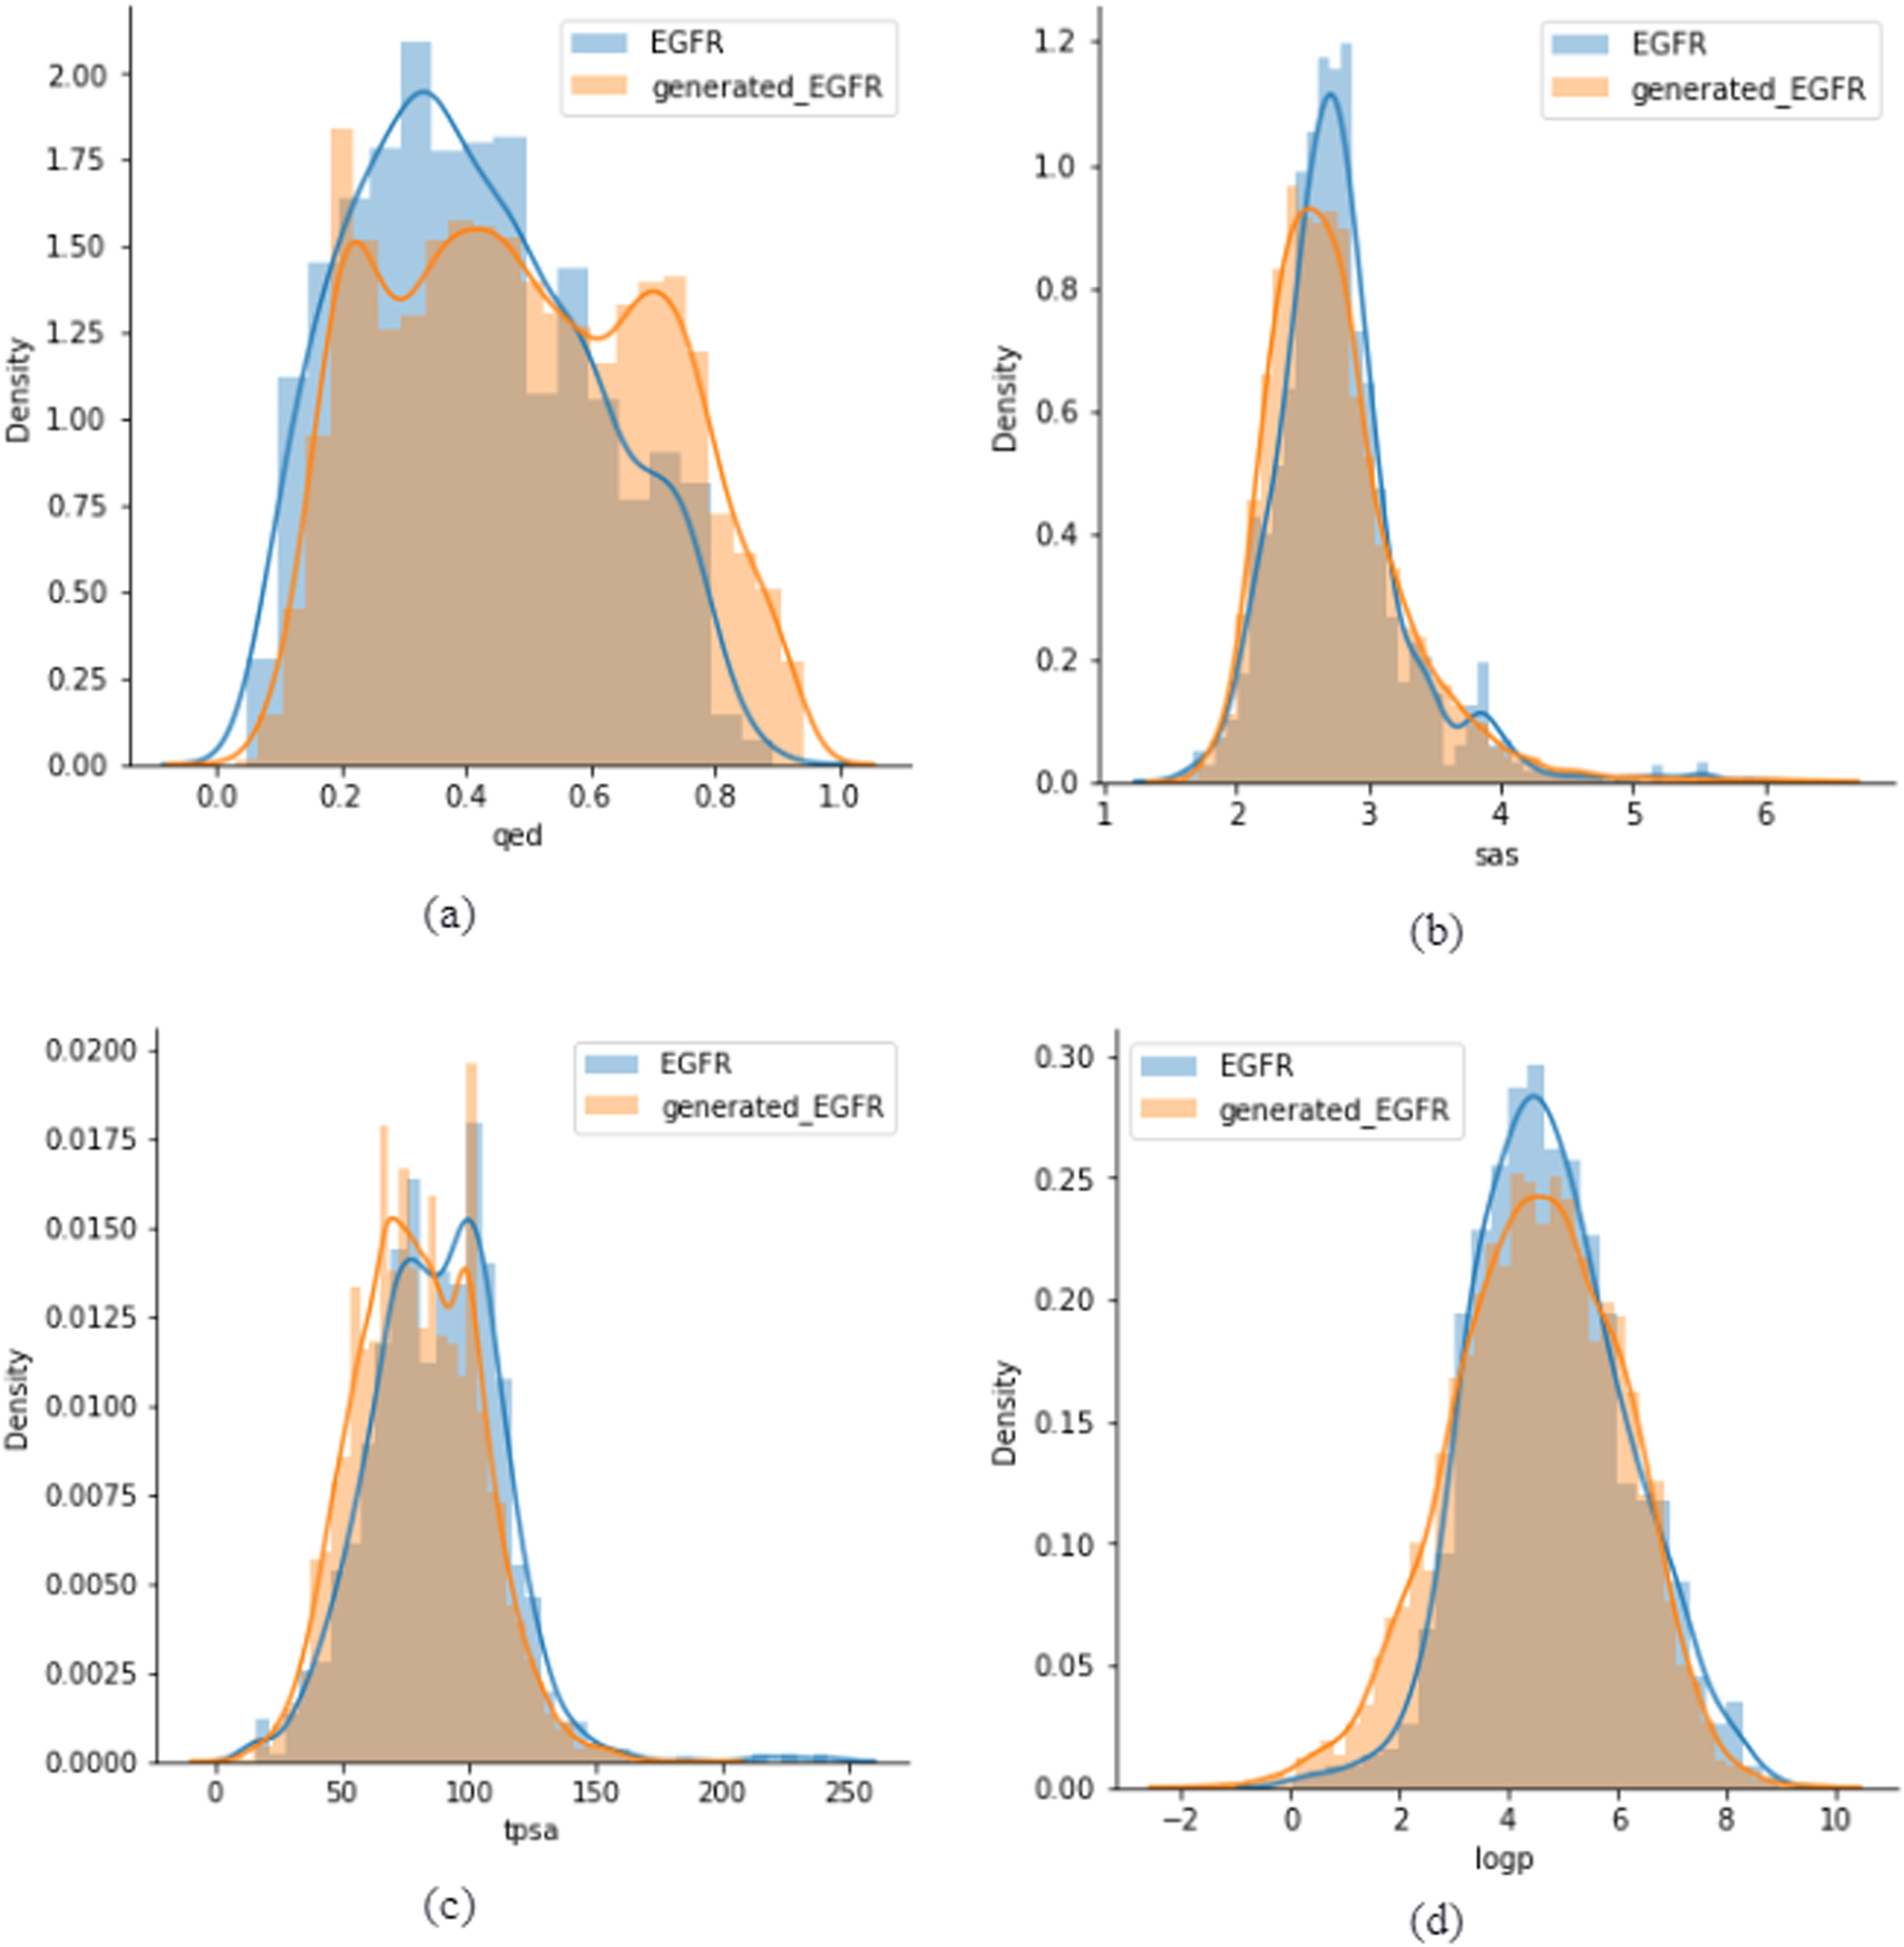
\includegraphics[width=\linewidth]{figures/9.png}
  \caption{EGFR 中分子的特性(QED、TPSA、SAS 和 logP)分布以及相对关注生成的分子}
  \label{fig:9}
\end{figure}

图 \ref{fig:9} 直观地表明生成的分子表现出与训练集相似的属性分布。

当使用 MOSES 数据集训练模型时,标准注意力的有效性为 99.4\%,而使用相对注意力时,有效性降至 99.2\%。同样,在 GuacaMol 数据集中,有效性从标准关注的 98.1\% 下降到相对关注的 97.8\%。当数据集足够大时,标准注意力足以学习 SMILES 所需的语法和语法。

然而,当应用于较小的特定目标数据集时,相对注意力的使用会带来更好的有效性。在表 9(采样的 S1PR1 数据集)中,有效性从 47\% 增加到 58.8\%。同样,在表 \ref{tab:11}(采样的 HTR1A 数据集)中,有效性从 85.2\% 提高到 86.3\%,在表 \ref{tab:13}(EGFR 数据集)中,有效性从 58.6\% 提高到 71.3\%。这些发现表明,当训练数据集大小有限时,利用相对注意力而不是标准注意力使模型能够更好地理解 SMILES 语法和化学规则。

当比较 GPT 模型与标准注意力和相对注意力在不同数据集上的性能时,当数据集足够大时,两种注意力机制都表现出相似的性能。然而,在使用迁移学习的小数据集进行特定目标药物设计的背景下,相对注意力比标准注意力有优势。

首先,它更好地捕获输入标记之间的依赖性,这在分子结构可以影响生物活性的药物设计中至关重要。通过考虑输入标记的相对位置,相对注意力可以准确地对它们的交互进行建模,从而改进预测。其次,相对注意力对于输入序列长度的变化更加稳健,这在处理训练样本有限的小数据集时很重要。

相比之下,标准注意力可能很难推广到不同长度的未见过的输入序列。 MolGPT 通过使用相对注意力来提高性能,特别是在小数据集上。这是因为它能够通过将相对位置信息纳入注意机制来更好地捕获序列中标记之间的关系。该模型生成了更多有效药物并更好地学习了数据统计。

通过应用迁移学习,该模型最初从更大的数据集(例如 MOSES)获取 SMILES 语法知识。随后,模型需要从更有限的数据集中适应和学习特定于目标特定药物的 SMILES 的语法。在这种情况下,相对关注被证明有利于促进学习的提高。它使模型能够快速掌握新的、未见过的标记的语法,这些标记可能存在于特定于目标的数据集中,但不存在于初始较大的数据集中。因此,与标准注意力相比,利用相对注意力的模型会生成更多数量的有效类药物分子,因为它能够从较小的数据集中更有效地学习这些新标记的语法。

\section{结论}

相对注意力是 Transformer 模型中使用的一种自注意力,已被证明可以增强需要标记相对位置的任务的性能,例如自然语言理解或图像字幕。它使模型能够捕获序列中不同位置之间的相互依赖性,而仅靠绝对位置编码和标准注意力可能无法捕获这些相互依赖性。

在这项研究中,我们利用变压器解码器模型中的相对关注来进行从头药物设计。我们的实验表明,具有相对关注度的 GPT 模型可以生成更有效、更独特、更新颖的药物,特别是当数据集很小且必须应用迁移学习时。模型中相对注意力的利用增强了 MOSES 数据集的新颖性,并提高了 GuacaMol 数据集的独特性。此外,我们证明了具有相对关注的模型可以学习和预测遵循训练集属性分布的分子。此外,该模型可以在条件生成过程中预测具有用户定义属性的分子。

当使用有限的数据集大小时,特别是在开发特定目标药物的背景下,使用相对注意力会显著提高模型性能。在评估具有相对关注的 MolGPT 模型在 MOSES 和 GuacaMol 数据集上的性能时,发现结果与具有标准关注的 MolGPT 所取得的结果相当。使用相对注意力的优势在这些数据集中并不那么明显,因为较大的数据集允许模型即使在标准注意力的情况下也能有效地学习 SMILES 语法。

通过利用 Huang 等人介绍的技术。为了计算相对位置编码,内存需求从 O(L$^2$D) 减少到 O(LD),其中 L 是序列长度,D 是隐藏状态维度。一个有前途的研究方向可能是使用相对位置编码和相对关注来学习目标蛋白质序列并生成具有改进的对接分数的分子。这将涉及将目标蛋白质序列作为模型的附加输入纳入其中。

应该指出的是,本研究中使用的模型仅仅是为了优化基本分子特性而设计的,并不能保证其在更复杂的任务(例如先导化合物优化)中的有效性。

\section{资金来源}

作者声明在手稿准备过程中没有收到任何赠款、资金或其他支持。

\section{作者贡献声明}

Suhail Haroon:概念化、方法论、软件、数据管理、写作 - 初稿。 Hafsath C.A.:写作 – 审阅和编辑、数据管理。 Jereesh A.S.:监督、项目管理。

\section{竞争利益声明}

无

\section{致谢}

无

\section{\textit{作者贡献}}

所有作者对这项工作做出了同等的贡献。所有作者阅读并认可终稿。

\printbibliography
\begin{translation-index}
\nocite{Haroon_C.a._A.s._2023}
\bibliographystyle{unsrtnat}
\printbibliography
\end{translation-index}
\end{translation}  % 本科生:外文资料的书面翻译
% \chapter{生物信息学与中医药的交叉融合 \\ ——中医药定量研究的数据科学和统计学方法}

\begin{center}
  作者:洪宇睿
\end{center}

\section*{摘要}
\begin{center}
  
  本调研报告聚焦于生物信息学与中医药交叉融合的研究领域,特别是中药化合物组分的初步数据收集与调研。在当前中医药研究中,化合物的定量数据不够完善,限制了药材鉴别和基于机器学习的处方优化的进展。本研究基于不同文献中的中药化合物数据,探讨了这些数据共同涉及的化合物,以评估基于现有文献的定量研究的可行性。通过对公开文献中的化合物定量数据进行初步收集与分析,本研究揭示了现有研究对化合物定量信息的收集和呈现方式不利于开展数据增强的现状,强调了进一步完善中药化合物定量数据的重要性,提供了利用现有数据进行对比分析的初步思路,为中医药定量研究提供了新的视角和方法。

\end{center}
\textbf{关键词:生物信息学;中医药;化合物定量;数据科学}

\section{研究背景}

中医作为一种历史悠久的医学体系,在现代医学领域逐渐受到重视。然而,中医药的研究与发展面临着一些固有的挑战。本研究背景部分将围绕中药材的化合物组分定量研究,探讨现有研究的局限性、挑战以及可能的解决途径。

中药的定量研究包括临床药代动力学、药材成分配比的质量检测、处方优化等多个方面。尽管这些研究为中医药的现代化发展提供了支持,但是对于药材与其效用之间准确的映射关系,尤其是基于古籍和临床实践的处方中药物作用的定量研究,仍然相对缺乏。这种研究的不足虽然有中医药的理论体系独特,涉及的药用成分极为复杂的客观原因,但也限制了中医药的研究验证,导致其长于“守正”而短于“创新”。\cite{Chen_Bi_Xie_Zhang_Shi_Guo_Yin_Zhang_Xin_Song_2021}

对于中药的化合物组分的定量研究,尤其是对于重要化合物的定量研究,目前仍然存在很多问题,如数据不完善、不可用、不可靠;现有关键组分的定量研究过程,往往依赖大量的临床记录首先确定关键药材,然后通过化学方法分离进行验证,这种方法在现有的临床数据支持下往往只能发现成分效果极其明显的单一药材,而对于往往由多种药材组成的复方,这种方法往往无法发现其中共同作用的关键组分。这些问题导致了中医药的定量研究的发展受到了很大的限制。\cite{Chu_Sun_Huang_Peng_Zhou_Zhang_2020}

进行大规模实验以定量刻画中药材化合物含量是解决上述问题的途径之一,但这种方法需要大量的资源和成本投入,使得研究实施变得复杂。为了解决高质量数据缺乏的问题,从公开文献中收集中医药信息成为一种可行的方法,这也是本调研的主要内容。在这个过程中,我们面临的主要挑战包括文献质量不一、数据组织形式不统一、化合物涉及范围有限、以及数据缺失问题。这些问题需要通过细致的数据清洗和增强来解决。

中药材的化合物组分受到生长环境、采收时间、加工方法等因素的影响,即使是同一品种的药材,其化合物含量也存在显著差异。这不仅是建立中药材化合物组分定量数据库的挑战,也是一个研究机遇。我们可以利用这种差异作为研究的突破点,将不同生长环境的中药材之间的含量差别作为同一物种的组内差别,从而更好地确定不同药材的组间差别,搜索药材的关键特征。

\section{研究方法}

\subsection{数据收集}

我们预期的完整结果是得到包括600余种中药材的化合物组分定量数据库,每组尽可能多地包含化合物的定量信息,包括尽可能广的化合物种类、不同文献对同一化合物组分的定量结果,以及同一篇文献对同一药材同一化合物所作的重复。其中,组内重复的主要形式有文献原始数据对同一植物物种的指定药用部位的重复、包含标准差的化合物均值,以及可视为不同批次的,同属异种或者同属同种不同亚种的药材的重复。在数据收集阶段,这些往往是我们能从文献中直接得到的结果。

具体的数据收集任务可以分为如下几个步骤:

\begin{itemize}
  \item 使用药材名或专有拉丁名称,或者植物学名,在文献数据库中搜索相关文献,并根据文章语义在文献中定位化合物定量数据。在此步骤中,可以依据目标数据集质量和规模的平衡,筛选特定期刊、影响因子等的文献。
  \item 根据具体的数据呈现形式进行数据处理。具体而言,一部分论文的补充材料中直接含有xlsx或者csv格式的原始数据;在线论文中的HTML数据表格可通过Table Converter Online等转换工具得到表格文件;对于只有PDF格式的文献,可以借助Mathpix Snipping Tool等OCR工具进行转换。
  \item 对于原始数据进行数据清洗。主要需要将数据中的单位统一,对含有标准差的均值记录标准差、样本容量以便后续重建分布,以及将原始宽数据转化为长数据,以便后续分析。
\end{itemize}

例如,对以下的数据表格:

\begin{figure}[H]
  \centering
  \includegraphics[width=0.8\textwidth]{figures/fig1.png}
  \caption{原始数据表格\cite{Jiang_Lan_Peng_Wang_Zhuang_2023}}
  \label{fig:fig1}
  常见的原始数据表格类型,其中除了含量信息(AN, TDS, AP, AK, SM),还包括一些对数据收集而言多余的列;组织形式为长数据,即不同种(LE, SI, TE, FE, FU)作为不同的数据列,需要转化成行长数据,即设置一个“学名”列,将不同种的数据均作为同一个表格中的记录,以“学名”列来标记所属。
\end{figure}

假设以$\mathrm{mg/kg}$作为统一的单位,经过Table Converter Online转换后及一些手动调整后,初步得到:

\begin{table}[H]
  \centering
  \begin{tabular}{|l|l|l|l|l|l|}
  \hline
      Species & LE & SI & TE & FE & FU \\ \hline
      AN & 45.013±8.24 & 54.447±6.655 & 64.547±7.178 & 33.153±5.345 & 26.883±6.694 \\ \hline
      TDS & 2543±121 & 9653±313 & 8470±1143 & 6943±574 & 6473±815 \\ \hline
      AP & 13.967±0.133 & 11.433±0.176 & 13.467±0.584 & 8.767±0.219 & 12.733±0.491 \\ \hline
      AK & 232.107±1.152 & 253.313±13.137 & 190.053±3.064 & 100.323±9.714 & 251.493±38.673 \\ \hline
  \end{tabular}
\end{table}

使用如下的R代码将其转化为长数据,并将标准差信息从均值中分离出来,添加上样本容量信息:

\lstset{basicstyle=\ttfamily, keywordstyle=\color[RGB]{40,40,255}, breaklines}

\begin{lstlisting}[language=R]
library(tidyverse)

# Read data
df <- read.csv("input.csv", header = TRUE, stringsAsFactors = FALSE)

# Convert wide data to long format, order by batch
df_long <- df %>%
  pivot_longer(
    cols = -Species, 
    names_to = "species", 
    values_to = "value"
  ) %>%
  mutate(
    batch = match(species, names(df)[-1]),
    compound = Species
  ) %>%
  select(batch, species, compound, value) %>%
  arrange(batch)

# Function to split mixed data into mean and std
split_data <- function(x) {
  parts <- strsplit(x, "±", fixed = TRUE)[[1]]
  mean <- as.numeric(trimws(parts[1]))
  std <- as.numeric(trimws(parts[2]))
  return(c(mean, std))
}

# Apply the function and create new columns
df_long <- df_long %>%
  mutate(
    mean = sapply(value, function(x) split_data(x)[1]),
    std = sapply(value, function(x) split_data(x)[2]),
    size = 3
  ) %>%
  select(-value)

# Output the result
write.csv(df_long, "output.csv", row.names = FALSE)
\end{lstlisting}

可以得到如下的长数据结果,这样就可以与其他文献中有关这一种中药的数据进行合并;收集到足够批次后,可以在数据中额外添加一个此药材的标签,再与其他药材的数据合并。这样就得到了格式严谨,既便于研究者阅读维护又便于计算机读取操作的化合物含量信息:

\begin{table}[H]
  \centering
  \begin{tabular}{|l|l|l|l|l|l|}
  \hline
      "batch" & "species" & "compound" & "mean" & "std" & "size" \\ \hline
      1 & "LE" & "AN" & 45.013 & 8.24 & 3 \\ \hline
      1 & "LE" & "TDS" & 2543 & 121 & 3 \\ \hline
      1 & "LE" & "AP" & 13.967 & 0.133 & 3 \\ \hline
      1 & "LE" & "AK" & 232.107 & 1.152 & 3 \\ \hline
      2 & "SI" & "AN" & 54.447 & 6.655 & 3 \\ \hline
      2 & "SI" & "TDS" & 9653 & 313 & 3 \\ \hline
      2 & "SI" & "AP" & 11.433 & 0.176 & 3 \\ \hline
      2 & "SI" & "AK" & 253.313 & 13.137 & 3 \\ \hline
      3 & "TE" & "AN" & 64.547 & 7.178 & 3 \\ \hline
      3 & "TE" & "TDS" & 8470 & 1143 & 3 \\ \hline
      3 & "TE" & "AP" & 13.467 & 0.584 & 3 \\ \hline
      3 & "TE" & "AK" & 190.053 & 3.064 & 3 \\ \hline
      4 & "FE" & "AN" & 33.153 & 5.345 & 3 \\ \hline
      4 & "FE" & "TDS" & 6943 & 574 & 3 \\ \hline
      4 & "FE" & "AP" & 8.767 & 0.219 & 3 \\ \hline
      4 & "FE" & "AK" & 100.323 & 9.714 & 3 \\ \hline
      5 & "FU" & "AN" & 26.883 & 6.694 & 3 \\ \hline
      5 & "FU" & "TDS" & 6473 & 815 & 3 \\ \hline
      5 & "FU" & "AP" & 12.733 & 0.491 & 3 \\ \hline
      5 & "FU" & "AK" & 251.493 & 38.673 & 3 \\ \hline
  \end{tabular}
\end{table}

\subsection{基于共有化合物的药材比对分析能力预测}

在这里,我们收集了刺五加等10种中药材的化合物含量信息(出于课题组的保密要求,具体表格未在这里给出),运用如下的代码检查了这些药材之间共有化合物的情况:

\begin{lstlisting}
suppressMessages(library(dplyr))
library(readxl)
options(tibble.print_max = Inf)
df <- read_excel('input.xlsx')

find_common_compounds_first_occurrence <- function(df) {
  # Add a column with row number to keep track of the original order
  df <- df %>% mutate(Row_Order = row_number())
  
  # Group by 'Compound' and 'Article_DOI', then summarize the first occurrence
  compound_first_occurrence <- df %>%
    group_by(Compound, Article_DOI, Latin_Name) %>%
    summarise(First_Occurrence = first(Row_Order)) %>%
    ungroup() # Ungroup to allow for the next operations
  
  # Count the number of unique DOIs for each compound
  compound_counts <- compound_first_occurrence %>%
    group_by(Compound) %>%
    summarise(Count = n_distinct(Article_DOI)) %>%
    filter(Count > 1) %>%
    select(Compound) # Select the compounds that appear in more than one paper
  
  # Join with the first occurrences
  common_compounds_first_occurrence <- compound_first_occurrence %>%
    inner_join(compound_counts, by = "Compound")
  
  return(common_compounds_first_occurrence)
}

common_compounds_first_occurrence <- find_common_compounds_first_occurrence(df)
print(common_compounds_first_occurrence)  
\end{lstlisting}


根据输出结果,共发现6种存在于两种药材中的具体化合物。假设任意两种药材之前出现相同化合物的种类期望是$\mathrm{E}$,则在数据集规模为$\mathrm{N}$时,新增的共享化合物配对数的期望可以用$\mathrm{NE}$来表示,这样,我们就可以求和得到规模$\mathrm{N}$的数据集所含的共享化合物配对数期望与为$\frac{N(N-1)}{2}E$,即与数据集规模的平成正比;平均每中药材与其他药材共享化合物的配对数期望为$(N-1)E$,即会线性增长,代入我们前10组数据得到的实际配对数,可以估计当数据集的规模为600时,每个化合物的平均配对数将达到80左右,药材的化合物组成将具有较高的交叉性。这种高度的交叉性为使用机器学习方法探究中药材的特征化合物提供了理论基础。通过统计不同药物之间出现相同化合物的组数,我们可以跨药材验证特定化合物是否可以作为区分两种或多种药材的关键指标。这种方法有助于深入理解中药材的化学特性和药效关系。

\subsection{基于方差分析的化合物特征性判断}

在得到数据集后,我们可以具体考察每一对含有公共化合物的药材,应用方差分析(ANOVA)来检验两组数据是否存在统计学上的显著差异,以判断这种公共化合物的含量是否可以成为区分这两种中药材的可靠特征。例如,在对岩白菜(BERGENIAE RHIZOMA)和枇杷叶(ERIOBOTRYAE FOLIUM)这两种中药中儿茶素(Catechin)含量的研究中,我们发现岩白菜的5个样本含量分别为2.4000\%,1.1300\%,2.0000\%,3.3100\%,2.8600\%\cite{Pandey_Kumar_Meena_Srivastava_Mishra_Tiwari_Pal_Nair_Upreti_Rana_2017},而枇杷叶的2个样本含量为1.2040\%和0.7344\%\cite{Chen_Zhang_Chen_2008},我们便可以检验儿茶素的含量是否可以区分这两种中药材。

应用现有成熟统计工具,的我们将使用单因素方差分析(One-Way ANOVA),它是一种统计技术,用于比较两个或多个样本均值是否存在显著差异,而不必进行多个两样本t检验。在单因素ANOVA中,我们假设所有组的总体均值相等,这是零假设(H0)。替代假设(H1)则是至少有一个组的均值与其他组不同。ANOVA通过比较组内方差(样本内部的变异)与组间方差(不同样本均值之间的变异)来决定是否拒绝零假设。

对于上面这个具体例子,我们运行以下的代码:

\begin{lstlisting}
bergeniae <- c(2.4000, 1.1300, 2.0000, 3.3100, 2.8600)
eriobotryae <- c(1.2040, 0.7344)
catechin_content <- c(bergeniae, eriobotryae)
herb_type <- factor(rep(c("Bergeniae", "Eriobotryae"),
                    times = c(length(bergeniae), length(eriobotryae))))
catechin_anova <- aov(catechin_content ~ herb_type)
summary(catechin_anova)

Df Sum Sq Mean Sq F value Pr(>F)  
herb_type    1  2.684   2.684   4.621 0.0843 .
Residuals    5  2.905   0.581                 
---
Signif. codes:  0 ‘***’ 0.001 ‘**’ 0.01 ‘*’ 0.05 ‘.’ 0.1 ‘ ’ 1
\end{lstlisting}

P值大于0.05但小于0.1,这意味着我们没有足够的证据在95\%的置信度下拒绝原假设。然而,这个P值落在了0.05到0.1之间,这在统计学上是一个边缘值,可以认为是有趋势性的证据表明两种药材中儿茶素含量存在差异,但这个证据不够强以确立显著性。在一些情况下,研究者可能会考虑接受更高的错误率(例如10\%),此时,我们可以说有显著性的趋势表明儿茶素含量可以作为区分这两种药材的特征。因此,我们要进行更多这样的方差分析来决定是否对数据集应用这样的策略,或者依然采用保守的0.05的P值门槛,认为根据ANOVA的结果,我们不能坚定地说儿茶素含量是区分岩白菜和枇杷叶的可靠特征。

目前的ANOVA是直接基于原始数值进行的,没有考虑样本量和标准差。如果我们有每个样本的标准差和样本量信息,我们可以采取以下额外的步骤来增强我们的分析:

\begin{itemize}
\item   \textbf{加权ANOVA}:当组间样本量差异较大时,使用加权均方和加权F值可以更准确地反映组间的差异。
\item   \textbf{元分析方法}:如果每个样本的标准差已知,可以应用元分析方法来综合考虑不同研究的结果,这在跨研究进行综合分析时尤其有用。
\item   \textbf{方差稳定性分析}:考虑到方差的稳定性是进行ANOVA的前提条件,如果每个样本的标准差已知,可以先进行方差齐性检验,如Levene's test或Bartlett's test。
\item   \textbf{数据分布重建}:通过均值和方差重建每个样本的数据分布(如假设数据服从正态分布),可以用来进行更复杂的模拟或蒙特卡洛方法,以估计实际的P值和效应量。
\end{itemize}

\section{总结}
在本研究中,我们探讨了生物信息学与中医药交叉融合的可能性,特别关注中药化合物组分的定量数据收集及其在药材鉴别和基于机器学习的处方优化中的应用。面对中医药定量数据的不完善性,我们通过公开文献收集了相关化合物的定量数据,并尝试使用数据清洗和增强的方法来提高数据质量和可用性。此外,我们还探索了数据集质量的评价和预测以及区分不同药材的关键指标的问题。

在研究方法中,我们详细描述了数据收集的多个步骤,包括文献搜索、数据转换和清洗。通过这些方法,我们尝试收集并整理了10种中药材的化合物数据,发现了6种在多种药材中共有的化合物,对随着数据集规模的增大,药材之间共有化合物的数量预期的增长趋势进行了预测,评估最终的数据集将能够符合应用机器学习方法的需要。

为了进一步验证化合物含量作为药材区分特征的有效性,我们岩白菜和枇杷叶中的儿茶素含量作为样例,采用了方差分析(ANOVA)来测试差异。尽管结果显示了这两种药材之间儿茶素含量的差异趋势,但没有达到统计学上的显著性标准,因此我们不能断定儿茶素含量是一个区分这两种药材的可靠特征,需要结合全数据集信息选择适合的显著性模板,这恰恰说明了中医药实际问题的复杂性。我们还认为采用更多其他统计方法进行尝试也对此问题具有一定的改进可能,将继续应用统计思想进行分析。

总而言之,本次调研为中医药定量研究提供了新的视角和方法,结合了数据科学中的三大要素——统计学、计算机科学和领域知识,对推动中医药与现代科学技术融合发展作出了自己的尝试。\cite{cite1}

% 致谢

% 声明
% 本科生开题报告不需要
\statement
% 将签字扫描后的声明文件 scan-statement.pdf 替换原始页面
% \statement[file=scan-statement.pdf]
% 本科生编译生成的声明页默认不加页脚,插入扫描版时再补上;
% 研究生编译生成时有页眉页脚,插入扫描版时不再重复。
% 也可以手动控制是否加页眉页脚
% \statement[page-style=empty]
% \statement[file=scan-statement.pdf, page-style=plain]

% 个人简历、在学期间完成的相关学术成果
% 本科生可以附个人简历,也可以不附个人简历
% % !TeX root = ../thuthesis-example.tex

\begin{resume}

  \section*{个人简历}

  2002 年 10 月 6 日出生于浙江省龙游县。

  2020 年 9 月考入清华大学探微书院化学生物学(药学方向)专业。


  % \section*{在学期间完成的相关学术成果}

  % \subsection*{学术论文}

  % \begin{achievements}
  %   \item Yang Y, Ren T L, Zhang L T, et al. Miniature microphone with silicon-based ferroelectric thin films[J]. Integrated Ferroelectrics, 2003, 52:229-235.
  %   \item 杨轶, 张宁欣, 任天令, 等. 硅基铁电微声学器件中薄膜残余应力的研究[J]. 中国机械工程, 2005, 16(14):1289-1291.
  %   \item 杨轶, 张宁欣, 任天令, 等. 集成铁电器件中的关键工艺研究[J]. 仪器仪表学报, 2003, 24(S4):192-193.
  %   \item Yang Y, Ren T L, Zhu Y P, et al. PMUTs for handwriting recognition. In press[J]. (已被Integrated Ferroelectrics录用)
  % \end{achievements}


  % \subsection*{专利}

  % \begin{achievements}
  %   \item 任天令, 杨轶, 朱一平, 等. 硅基铁电微声学传感器畴极化区域控制和电极连接的方法: 中国, CN1602118A[P]. 2005-03-30.
  %   \item Ren T L, Yang Y, Zhu Y P, et al. Piezoelectric micro acoustic sensor based on ferroelectric materials: USA, No.11/215, 102[P]. (美国发明专利申请号.)
  % \end{achievements}

\end{resume}


% 指导教师/指导小组评语
% 本科生不需要
% \input{data/comments}

% 答辩委员会决议书
% 本科生不需要
% \input{data/resolution}

% 本科生的综合论文训练记录表(扫描版)
% \record{file=scan-record.pdf}

\end{document}
